% Final technical report: synthetic Bengali handwriting (page layout + word generation)
% Build: latexmk -xelatex report.tex      Charts: python make_figs.py
\documentclass[10.5pt,a4paper]{article}
\usepackage[margin=2.2cm,top=2.3cm,bottom=2.4cm]{geometry}
\usepackage{fontspec}
\setmainfont{Liberation Serif}
\setsansfont{Liberation Sans}
\setmonofont{DejaVu Sans Mono}[Scale=0.82]
\newfontfamily\bn[Script=Bengali,Path=/home/hpc4090/shyan/ocr/scribe_layout_v2/bscribe_shim/]{NotoSansBengali.ttf}
\usepackage{amsmath,amssymb}
\usepackage{booktabs,multirow,makecell,longtable,threeparttable}
\usepackage{graphicx,float,placeins}
\usepackage[font=small,labelfont=bf]{caption}
\usepackage{subcaption}
\usepackage[dvipsnames]{xcolor}
\usepackage{tikz}
\usetikzlibrary{arrows.meta,positioning,fit,backgrounds,calc}
\usepackage{enumitem}
\setlist{itemsep=1pt,topsep=3pt}
\usepackage{microtype}
\usepackage{fancyhdr}
\usepackage[colorlinks=true,linkcolor=MidnightBlue,citecolor=MidnightBlue,urlcolor=MidnightBlue]{hyperref}
\pagestyle{fancy}\fancyhf{}
\fancyhead[L]{\small Synthetic Bengali handwriting: final report}
\fancyhead[R]{\small\thepage}
\renewcommand{\headrulewidth}{0.3pt}
\setlength{\parskip}{3pt}
\renewcommand{\arraystretch}{1.12}
\graphicspath{{figs/}}

% ---- macros ----------------------------------------------------------------
\newcommand{\fp}[1]{\nolinkurl{#1}}
\newcommand{\src}[1]{\par\vspace{1pt}{\footnotesize\textcolor{gray}{Source:} #1\par}}
\newcommand{\Bp}{B$'$}
\newcommand{\Ap}{A$'$}
\newcommand{\U}{\,U}
\newcommand{\ci}[2]{{\footnotesize[#1,\,#2]}}
\newcommand{\pend}{\textcolor{BrickRed}}
\newcommand{\bnt}[1]{{\bn #1}}

\title{\textbf{Synthetic Bengali Handwriting:\\ Learned Page Layout and Writer-Conditioned Word Generation}\\[4pt]
\large Final technical report}
\author{scribe\_layout / scribe\_layout\_v2 / scribe\_wordgen projects}
\date{19 October 2026}

\begin{document}
\maketitle

\begin{abstract}
\noindent BengaliScribe synthesises handwritten Bengali pages by generating word images with a font-prior GAN (baseline
\emph{B0}) and pasting them onto a page with hand-picked layout constants. Its pages look \emph{typeset in a handwriting-like
font}: the words re-ink a NotoSans skeleton with a stroke about 55\% wider than the target writer's, and the lines are evenly
spaced and straight. This report covers two lines of work. (1)~\textbf{Page layout.} We measured how real writers lay out
words on 963 full-page scans and trained a small page-autoregressive mixture-density model (v1, then v2). The final default
(v2 \texttt{default\_unfitw\_dc}) reaches a plan-level line C2ST AUC of $0.535\pm0.012$ on unseen texts (v1: $0.566\pm0.021$;
hand-tuned layout: 0.980; within-page null 0.496). Two spectral side-studies are reported with their corrections.
(2)~\textbf{Word generation.} We built a few-shot latent-diffusion word generator from DiffusionPen and a full evaluation suite.
That suite has a locator CER, an independent CRNN recogniser (R\_eval), writer-ID style metrics (E\_eval/E\_shape) and a
sub-pixel pen metric. All statistics use writer-bootstrap CIs. The best diffusion arm, \textbf{S} (pen knob plus reference
tokens in decoupled cross-attention), ties B0 on locator CER and on style MRR (0.579 vs 0.596), with a matched pen after
calibration. Under R\_eval it is still \emph{less legible} than B0 ($+0.033$ \ci{+0.015}{+0.052} codepoint CER on words of
$\ge$3 codepoints). Pretraining R\_eval on renders from 48 Bengali fonts helps a little with full data and a lot with 10\% of
the writers. Every number in this report is traced to a result file. Three experiments still running are listed only as
next steps.
\end{abstract}

\tableofcontents
\newpage

%=============================================================================
\section{Executive summary}
\label{sec:exec}

\paragraph{Key findings.}
\begin{itemize}
\item \textbf{B0's ``font look'' is architectural, not a training accident.} B0 keeps fine-resolution skips from a NotoSans
  prior. Its only deformation module can move ink at most 1.4\,px vertically on a 64-px canvas. Its losses reward the averaged
  font skeleton. Generated page strokes are 0.39\,mm wide against 0.25\,mm real (\S\ref{sec:intro}).
\item \textbf{The learned layout beats hand-tuned constants by a wide margin and v1 by a small one.} The plan-level line C2ST
  is 0.980 for manual, $0.566\pm0.021$ for v1 and $0.535\pm0.012$ for the v2 default on TEST ($0.536\pm0.027$ on VAL). End to
  end, through BengaliScribe and the real detector, v2 scores a line C2ST of 0.719 (0.619 with writer context), against 0.905
  for manual and a floor of 0.534 (\S\ref{sec:layout}).
\item \textbf{Several layout gains were measurement artefacts and were corrected.} Corrected items are a biased end-to-end C2ST
  (floor 0.34 instead of 0.5), per-word wobble overshoot, selection on TEST, and a Fourier ``17$\times$ better'' claim. In the
  fair comparison, Fourier and v1 are equal, 0.668 vs 0.702 (\S\ref{sec:spectral}).
\item \textbf{Diffusion fixes the texture but had to earn legibility.} The first DiffusionPen probe wrote round, flowing,
  handwriting-like strokes, but its locator CER was 0.65--0.97. Content tokens in cross-attention, full data, white-paper
  normalisation and a fixed classifier-free-guidance (CFG) null brought \Bp{} to 0.188 at g3. That fix was a bug fix: content
  had sat in both CFG branches. A guidance of t5c5 then reached 0.148, against 0.130 for B0 (\S\ref{sec:wordgen}).
\item \textbf{Arm S is the best diffusion arm.} It ties B0 on locator CER ($+0.007$ \ci{-0.023}{+0.040}) and on style M2 MRR
  ($-0.017$ \ci{-0.116}{+0.088}). It beats P on style by $+0.136$ \ci{+0.085}{+0.187} (17/20 writers). Its pen is 1.13 raw and
  1.06 calibrated (\S\ref{sec:armsPS}).
\item \textbf{R\_eval changes the CER picture.} The locator was too weak to separate arms. With R\_eval, S$-$B0 is $+0.059$
  \ci{+0.036}{+0.083} on all words and $+0.033$ \ci{+0.015}{+0.052} on words of $\ge$3 codepoints. Part of the all-word gap
  is a short-word \texttt{img\_to\_ink} artefact; the $\ge$3-codepoint gap remains significant (\S\ref{sec:rescore}).
\item \textbf{Recogniser CER measures legibility, not fidelity.} B0 scores \emph{better than the real crops} under R\_eval
  ($-0.014$ \ci{-0.027}{-0.002}). CER is therefore a floor check and must be read alongside style and pen.
\item \textbf{Fonts are a useful recogniser prior, mostly when real data is scarce.} Fonts$\to$real fine-tuning gives
  $-0.004$ \ci{-0.008}{-0.002} VAL CER with all writers and $-0.063$ \ci{-0.080}{-0.054} with 10\% of the writers. Fonts
  alone give 0.456 and do not transfer (\S\ref{sec:fonts}).
\end{itemize}

\begin{table}[H]
\centering
\caption{Current best, word generation (VAL, 20 writers, 781 targets). CER (locator) is letter-unit and per-word-mean.
R\_eval CER is codepoint and corpus-level. \textbf{The two CER columns are in different units; do not compare them.} Style is
M2 MRR (E\_eval; chance 0.28). Pen is the generated/own-writer sub-pixel width-per-core ratio (1.00 = match). CIs are 95\%
writer-bootstrap.}
\label{tab:best}
\small
\begin{tabular}{@{}lcccccc@{}}
\toprule
arm & locator CER & R\_eval CER all & R\_eval CER $\ge$3cp & style M2 MRR & M2s MRR & pen raw / cal \\
\midrule
real & 0.133 \ci{0.100}{0.167} & 0.0438 \ci{0.031}{0.059} & 0.0424 \ci{0.029}{0.057} & 0.821 \ci{0.775}{0.859} & 0.768 & 1.00 \\
B0   & 0.130 \ci{0.103}{0.156} & 0.0302 \ci{0.025}{0.036} & 0.0226 \ci{0.016}{0.029} & 0.596 \ci{0.488}{0.711} & 0.533 & 1.15 \\
\textbf{S t5c5} & 0.137 \ci{0.101}{0.174} & 0.0889 \ci{0.065}{0.115} & 0.0552 \ci{0.038}{0.075} & \textbf{0.579} \ci{0.521}{0.635} & 0.517 & 1.13 / 1.06 \\
P t5c5 & 0.132 \ci{0.097}{0.171} & 0.0905 \ci{0.066}{0.118} & 0.0577 \ci{0.040}{0.079} & 0.443 \ci{0.379}{0.505} & 0.416 & 1.15 / 1.06 \\
\Bp{}v2 t5c5 & 0.151 \ci{0.117}{0.186} & 0.1412$^{\dagger}$ & 0.1024$^{\dagger}$ & 0.418 \ci{0.355}{0.483} & 0.399 & 1.29 / 1.07 \\
\bottomrule
\end{tabular}
\par\smallskip\footnotesize $^{\dagger}$From the full R\_eval rescoring table in \fp{runs/R_eval/full_chain.log} (\texttt{Bv2\_t5c5}: 0.1412 \ci{0.1125}{0.1749} all words, 0.1024 \ci{0.0823}{0.1272} $\ge$3cp); \fp{RESULTS.md} lists only the default subset of arms. Checkpoints: S
\fp{runs/P1a3/S/}, P \fp{runs/P1a3/P/}, \Bp{} \fp{runs/P1a2/B/}, B0 = BengaliScribe \texttt{models/v2}.
\src{\fp{runs/P1a3/eval/report_tables.txt}, \fp{runs/P1a3/eval/metrics.json}, \fp{runs/R_eval/RESULTS.md}, \fp{EXPERIMENTS.md}
(all under \fp{scribe_wordgen/})}
\end{table}

\begin{table}[H]
\centering
\caption{Current best, page layout. Lower AUC = closer to real; 0.5 = indistinguishable. Plan level: 193 TEST pages (unseen
texts), 5 seeds, mean $\pm$ sd. End to end: 5 writers $\times$ 2 seeds, balanced C2ST.}
\label{tab:bestlayout}
\small
\resizebox{\linewidth}{!}{\begin{tabular}{@{}lcccc@{}}
\toprule
layout & plan line C2ST (TEST) & plan line C2ST (VAL) & plan page C2ST (TEST) & e2e line / page C2ST \\
\midrule
manual (BengaliScribe constants) & 0.980 & -- & 1.0 & 0.905 / 0.999 \\
v1 (\fp{scribe_layout/runs/default}) & $0.566\pm0.021$ & $0.560\pm0.024$ & $0.654\pm0.043$ & -- \\
\textbf{v2 default} (\fp{default_unfitw_dc}) & $\mathbf{0.535\pm0.012}$ & $0.536\pm0.027$ & $0.590\pm0.024$ & 0.719 / 0.850 \\
v2 default + writer context & -- & -- & -- & 0.619 / 0.845 \\
null: within-page split / e2e real halves & $0.496\pm0.019$ & -- & -- & 0.534 / 0.508 \\
\bottomrule
\end{tabular}}
\src{\fp{scribe_layout_v2/runs/compare_unfitw/compare_5seed{,_dc,_val}.txt}, \fp{scribe_layout_v2/report/FACTS.md},
\fp{scribe_layout_v2/runs/e2e_final/results.md}}
\end{table}

%=============================================================================
\section{Introduction and motivation}
\label{sec:intro}

BengaliScribe (BS) turns a text into a handwritten-looking page in three steps. It reads the target writer's reference
crops with an attention locator (\texttt{attn\_locator}). It generates each word with a font-prior GAN conditioned on a
style vector (\texttt{font\_generator\_pilot\_sal.py}, ``FG''). It then lays the words out with hand-picked constants
(\texttt{write\_page.py}, ``WP''). We call the shipped generator \textbf{B0}. Our showcase writer is \texttt{image\_2}, a
page from the hcr/996 corpus that no model trains on. Its hand is thin, sparse, rounded and cursive. B0's output for it is
bold, uniform and angular: a re-inked font skeleton.

\subsection{Why B0 looks like a font}
The planning diagnosis (\fp{PLAN.md} \S1) was checked line by line by an adversarial review (\fp{PLAN_REVIEW.md} \S0). It
found these causes:
\begin{enumerate}
\item \textbf{The architecture copies the font.} FG is a 4.6\,M-parameter U-Net over the NotoSans render (the checkpoint
  holds 4.587\,M). It keeps the 1/4- and 1/2-resolution skips (\texttt{SKIP\_SCALES=(1,1,0)}), so stroke positions reach the
  decoder with 2-px precision. The only module that moves ink is \texttt{StyleWarp}. A bound on its learned weights gives at
  most 1.38\,px vertical and 5.75\,px horizontal displacement on the $64\times256$ canvas; the architectural cap is
  3.84/15.4\,px. An i-kar loop of the reference writer rises 0.87 core (median) above the matra, which is out of reach.
  Cross-attention to the references is off (\texttt{XATTN=False}).
\item \textbf{The losses reward an averaged font skeleton.} The loss is $4\,L_1 + 1\cdot$LSGAN $+ 0.3\,$style-CE
  $+ 0.3\,$CTC. The $L_1$ term is salience-weighted on both target and font, and the PatchGAN is conditioned on the prior.
  When prior and target are misaligned beyond the warp's range, the $L_1$ optimum is a blurred stroke along the font skeleton.
\item \textbf{Train/inference mismatch in width.} In training the prior is resized into the target's box. At inference it
  keeps the font's natural width, so word width and letter spacing are copied from the font.
\item \textbf{Resolution and pen are set by the data, not the writer} (Table~\ref{tab:penwidth}). The reference writer's
  stroke-to-core ratio (0.053) is below BN-HTR's 10th percentile. At 64\,px it is about 1.6\,px wide, which the canvas cannot
  render sharply. \texttt{crop\_ink} also stretches every target so its 5th-percentile pixel is fully black, so darkness
  saturates: 0.93 generated against 0.80 real.
\end{enumerate}
The measured outcome on the page is a stroke of \textbf{0.39\,mm generated against 0.25\,mm real}, about 55\% wider
(\fp{PLAN.md} \S1.4, orchestrator measurement).

\begin{table}[H]
\centering
\caption{Stroke width relative to letter size (skeleton EDT width $\div$ body height from \texttt{measure\_rows}), by data
set. image\_2 is the reference writer.}
\label{tab:penwidth}
\small
\begin{tabular}{@{}lrccc@{}}
\toprule
set & crops & width/core median (IQR) & native crop height & darkness \\
\midrule
BN-HTR (B0's training data) & 1489 & 0.106 (0.077--0.185) & 74 px & 0.98 \\
BanglaWriting & 1497 & 0.090 (0.066--0.135) & 163 px & 1.00 \\
hcr/996 (60 pages) & 1447 & 0.075 (0.060--0.103) & 102 px & 0.82 \\
\textbf{hcr image\_2 (reference writer)} & 57 & \textbf{0.053} (0.048--0.067) & 107 px & 0.79 \\
generated for image\_2 (64-px canvas) & 60 & 0.063 (0.045--0.076) & 64 & 0.97 \\
\bottomrule
\end{tabular}
\src{\fp{scribe_wordgen/PLAN.md} \S1.4 (script \fp{scratch/pen_ratio.py}; re-run identically in \fp{PLAN_REVIEW.md} \S0)}
\end{table}

Per-writer BN-HTR medians span 0.073--0.186 (p10--p90 over 110 writers). The second problem is \textbf{layout}. WP places
words with uniform random gaps, a tiny fixed line slope, and a fixed pitch of $2.7\times$ body height, so every line is
straight and evenly spaced.

\subsection{Goal and overall design}
The goal is a page generator that \emph{writes like the reference writer}: the writer's letter construction and pen, laid
out the way real people lay out lines. Figure~\ref{fig:pipeline} shows the pieces built in this project and how they are
evaluated. Each evaluator is independent of the generator it scores: none is ever used as a training loss.

\begin{figure}[H]
\centering
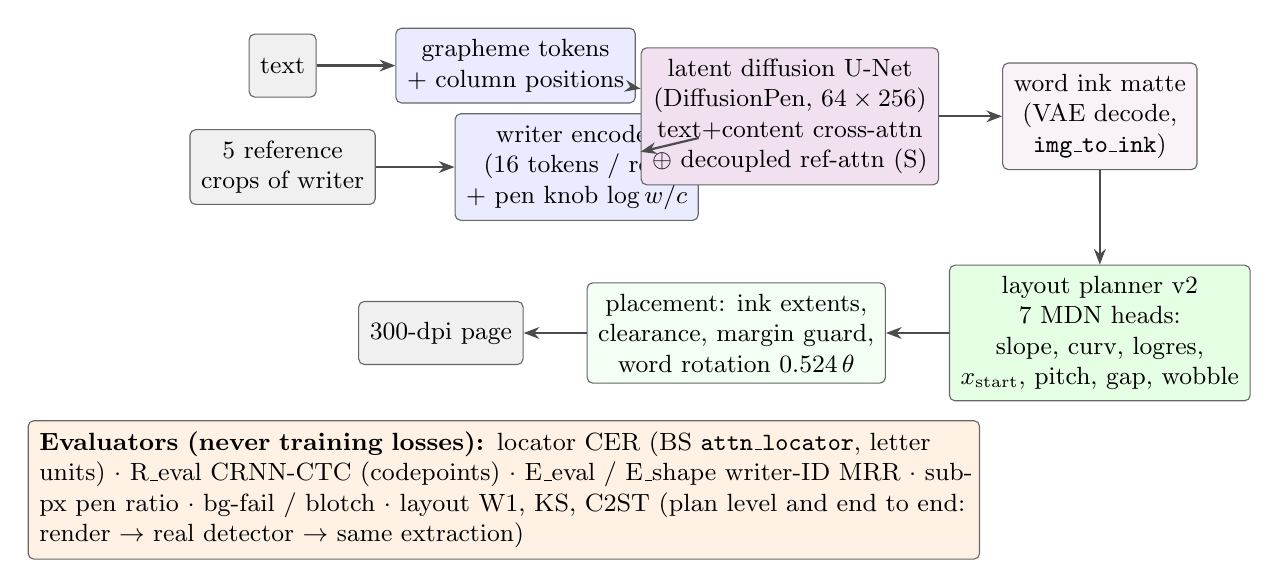
\begin{tikzpicture}[
  font=\small, node distance=4mm and 7mm,
  box/.style={draw=black!60, rounded corners=2pt, fill=#1, align=center, inner sep=4pt, minimum height=8mm},
  box/.default=white, arr/.style={-{Stealth[length=2mm]}, black!70, thick}]
\node[box=gray!12] (text) {text};
\node[box=gray!12, below=of text] (refs) {5 reference\\crops of writer};
\node[box=blue!8, right=10mm of text] (tok) {grapheme tokens\\+ column positions};
\node[box=blue!8, right=10mm of refs] (enc) {writer encoder\\(16 tokens / ref)\\+ pen knob $\log w/c$};
\node[box=violet!12, right=12mm of $(tok)!0.5!(enc)$, minimum width=34mm] (unet) {latent diffusion U-Net\\(DiffusionPen, $64\times256$)\\text+content cross-attn\\$\oplus$ decoupled ref-attn (S)};
\node[box=violet!5, right=8mm of unet] (ink) {word ink matte\\(VAE decode,\\\texttt{img\_to\_ink})};
\node[box=green!10, below=12mm of ink] (plan) {layout planner v2\\7 MDN heads:\\slope, curv, logres,\\$x_\mathrm{start}$, pitch, gap, wobble};
\node[box=green!5, left=8mm of plan] (place) {placement: ink extents,\\clearance, margin guard,\\word rotation $0.524\,\theta$};
\node[box=gray!12, left=8mm of place] (page) {300-dpi page};
\draw[arr] (text) -- (tok); \draw[arr] (refs) -- (enc);
\draw[arr] (tok) -- (unet); \draw[arr] (enc) -- (unet); \draw[arr] (unet) -- (ink);
\draw[arr] (ink) -- (plan); \draw[arr] (plan) -- (place); \draw[arr] (place) -- (page);
\node[box=orange!10, below=7mm of page, xshift=8mm, text width=118mm, align=left] (ev) {\textbf{Evaluators (never training losses):}
locator CER (BS \texttt{attn\_locator}, letter units) $\cdot$ R\_eval CRNN-CTC (codepoints) $\cdot$ E\_eval / E\_shape
writer-ID MRR $\cdot$ sub-px pen ratio $\cdot$ bg-fail / blotch $\cdot$ layout W1, KS, C2ST (plan level and end to end:
render $\to$ real detector $\to$ same extraction)};
\end{tikzpicture}
\caption{The system. Upper row: the word generator (Arm S configuration; Arm P lacks the reference-token attention). Lower
row: the learned layout and its placement rules. Bottom: the evaluators.}
\label{fig:pipeline}
\end{figure}

%=============================================================================
\section{Data and protocol}
\label{sec:data}

\subsection{Data sets}
\begin{table}[H]
\centering
\caption{Data sources. Only BN-HTR and BanglaWriting are used to train word models. hcr/996 is used for layout and as an
evaluation-only showcase (image\_2).}
\label{tab:data}
\small
\begin{tabular}{@{}p{2.6cm}p{2.6cm}p{1.6cm}p{2.0cm}p{6.0cm}@{}}
\toprule
source & word crops & writers & native size & notes \\
\midrule
BN-HTR & 92,380 labelled + filtered (from 108,181) & 149 & median crop h 74\,px, core $\approx$28--30\,px & 93,758 labelled and $\le$16 graphemes, minus 1,378 flagged by \texttt{label\_filter.json}; folder = writer \\
BanglaWriting (BW) & 20,523 & 260 (\texttt{style\_id} = page = person) & median crop h 163\,px, core $\approx$49\,px & one page per writer; manual labels \\
hcr/996 & $\approx$48.7k word pieces & unknown & A4, 300\,dpi, core median 41\,px & 27 texts copied by many writers; 963 usable pages for layout; no writer IDs \\
\bottomrule
\end{tabular}
\src{\fp{scribe_wordgen/PLAN.md} \S1.6, \S2.1; \fp{runs/T0/REPORT.md}; \fp{scribe_layout/report/scribe_layout_report.tex} \S2}
\end{table}

\subsection{Writer-disjoint splits}
Splits are fixed in \fp{data_cache/splits.json}, and a test asserts that no writer appears in two of them (\fp{runs/T0/REPORT.md}):
\begin{itemize}
\item \textbf{BN-HTR:} TEST = \{15, 22, 24, 28, 30, 48, 51, 54, 69, 136\} (5,768 crops); VAL = \{99, 117, 127, 142, 149\};
  TRAIN = the remaining 134 writers. TEST writers are in BS's generator and locator hold-out, so B0 is scored on writers it
  never saw. The VAL writers are in the TRAIN set of BS's style encoder \texttt{ms4}; this was verified, not assumed
  (\fp{PLAN_REVIEW.md} \S0).
\item \textbf{BanglaWriting:} \texttt{style\_id}s hash-sorted (SHA-256) into 220 TRAIN / 15 VAL / 25 TEST.
  \texttt{dp\_words\_b64} (baseline B3) saw all 260 BW writers, so B3 is fair only on BN-HTR.
\item \textbf{hcr/996 (layout):} split \emph{by source text}: 18 train / 4 val / 5 test texts (test texts \{4, 6, 11, 15,
  18\}), giving 614 / 144 / 193 pages. The v1 report claimed test lines are by unseen writers. The v2 review notes that
  writers likely repeat across texts, which cannot be checked without writer IDs (\S\ref{sec:contradictions}).
\end{itemize}

\subsection{The VAL protocol (word generation)}
Unless stated otherwise every word-generation number uses this protocol (\fp{EXPERIMENTS.md}, header):
\begin{itemize}
\item \textbf{20 VAL writers}: the 5 BN-HTR VAL writers plus the 15 BW VAL writers, with \textbf{781 target words} in total.
\item \textbf{5 conditioning references per writer.} For BN-HTR these come from page A and the targets from other pages. For
  BW the refs and targets come from the same (only) page, which inflates BW style metrics through page cues
  (\fp{runs/P1a/REVIEW.md} \S4).
\item Targets whose text is among the refs are excluded. Punctuation-only targets (54/781, all BW) are excluded from the
  headline CER.
\item \textbf{Seeds.} B0 and real have one sample per word. Diffusion arms have two seeds from eval\_v3 onward. Paired
  comparisons merge on (dataset, writer, idx, seed\_k) and never zip lists.
\end{itemize}

\subsection{TEST status}
\textbf{No generator has been evaluated on TEST.} The final TEST evaluation (Checkpoint C) has not been run. The only TEST
contact is that the independent recogniser R\_eval was scored once on real TEST crops (7,665 words, \S\ref{sec:fonts}). For
layout, all design choices were compared on TEST (selection on test). A selection-free VAL check was run afterwards
(\S\ref{sec:layoutval}).

\subsection{Data-handling facts that affect the numbers}
\begin{itemize}
\item \textbf{The BanglaWriting word-crop PNGs are missing from disk.} The files under
  \fp{Diffusion_model_dataset_building/dataset/word_crops/} that \fp{index_bw.csv} points to were deleted. The script
  \fp{wordgen/recog/bw_regen.py} rebuilds the crops in memory from the LabelMe page JSON and JPG in
  \fp{banglawriting/converted/}. It is a faithful port of the original \texttt{parse\_json}/\texttt{crop\_box} and
  label-checks every crop.
\item \textbf{R\_eval BW coverage.} The R\_eval real-crop cache holds \textbf{20,482 of the 20,523} BW words (17,539 TRAIN +
  1,046 VAL + 1,897 TEST rows in \fp{runs/R_eval/cache/bw_*.jsonl}). The 41 missing words are the rows that already failed
  \texttt{measure\_rows} in the T0 data index (\fp{runs/T0/REPORT.md} \S4.2: ok 20,482 of 20,523); the cache's per-split
  counts equal T0's ok-row counts.
\item \textbf{Core-normalised canvas: clip target not met.} The plan's 160-px core-normalised canvas (core 32\,px) clipped
  22.6\% of BN-HTR and 21.1\% of BW TRAIN crops, almost all at the top (\fp{runs/T0/REPORT.md} \S4.3). A writer-prior fallback
  cut this to 18.98\% / 14.57\% (\fp{runs/T0b/REPORT.md}), still far from the $<$1\% target. The SD-VAE round trip also fails
  the plan's IoU gate ($\ge$0.93) at core 32 (image\_2 0.862; \fp{PLAN_REVIEW.md} B1). All generators therefore stayed on
  DiffusionPen's height-normalised $64\times256$ \texttt{fit\_canvas}. The learned layout rescales words by measured core
  anyway.
\end{itemize}

%=============================================================================
\section{Evaluation methodology}
\label{sec:eval}

Every word metric is computed per writer and then averaged over writers. The CI is a writer-level bootstrap: 2,000
resamples, 95\% percentile interval. A ``tie'' means the paired CI includes 0.

\subsection{Locator CER (letter units, per-word mean)}
BS's frozen \texttt{attn\_locator} reads each word on a fixed $64\times256$ canvas. The ink is tight-cropped and
left-aligned; wider words are resized to fit (eval\_v3 truncated B0 words wider than 256\,px, which affects about 10\% of
B0). For target $y_i$ and reading $\hat y_i$,
\begin{equation}
\mathrm{CER}^{\mathrm{loc}}_i=\min\!\Big(1,\ \frac{d_{\mathrm{edit}}(\hat y_i,y_i)}{|y_i|}\Big),\qquad
\mathrm{CER}^{\mathrm{loc}}_w=\frac{1}{|T_w|S}\sum_{i\in T_w}\sum_{s}\mathrm{CER}^{\mathrm{loc}}_{i,s},\qquad
\mathrm{CER}^{\mathrm{loc}}=\frac{1}{20}\sum_w \mathrm{CER}^{\mathrm{loc}}_w .
\end{equation}
The edit distance is in the locator's letter units. The cap at 1 matters: without it, garbage reads of 1-character
punctuation targets gave CERs of 23--29 and 15\% of words had CER $>1$ (\fp{runs/P1a/REVIEW.md} \S1). The locator is
BN-HTR-trained. Its own real-crop CER is 0.056 on BN-HTR VAL and 0.236 on BW VAL (\fp{runs/R_eval/RESULTS.md}), so it
separates arms poorly on BW.

\subsection{R\_eval CER (codepoints, corpus level)}
R\_eval is an independent CRNN-CTC recogniser (\S\ref{sec:fonts}). Its CER is micro-averaged over Unicode codepoints and
not capped:
\begin{equation}
\mathrm{CER}^{R}=\frac{\sum_i d_{\mathrm{edit}}(\hat y_i,y_i)}{\sum_i \max(|y_i|,1)} ,
\end{equation}
where $|\cdot|$ counts codepoints. The CI resamples writers and recomputes the corpus ratio. A paired difference
$\mathrm{CER}^R(a)-\mathrm{CER}^R(b)$ is computed on the same rows (same gold, same writer) and bootstrapped the same way
(\fp{wordgen/recog/metrics.py}). Results are reported for all words and for words of $\ge$3 codepoints. \textbf{Locator CER
and R\_eval CER differ in unit (letters vs codepoints) and in aggregation (capped per-word mean vs corpus ratio). They must
never be compared with each other.}

\subsection{Style: writer-identification MRR (M2, M2s)}
E\_eval and E\_shape are ResNet-18 writer-embedding networks trained with SupCon plus cosine-softmax CE, on TRAIN writers
only. \textbf{E\_eval} sees the normalised ink matte (construction \emph{and} pen). \textbf{E\_shape} sees a spur-pruned
skeleton redrawn at a fixed thin width (construction only). Every source goes through one preprocessing path that ends at
the generators' $64\times256$ canvas (\fp{wordgen/eval/writer_id.py}). For a query word $q$ of writer $w$, each candidate
writer $v$ of the same dataset has a gallery vector $g_v$: the L2-normalised mean embedding of real crops disjoint from
the refs and the query. The galleries are cross-fitted by index parity, and crops with the query's text are removed. With
$r_q$ the rank of $w$ among candidates by $\cos(e_q,g_v)$:
\begin{equation}
\mathrm{MRR}=\frac{1}{20}\sum_w\frac{1}{|Q_w|}\sum_{q\in Q_w}\frac{1}{r_q},\qquad
\mathrm{margin}_q=\cos(e_q,g_w)-\max_{v\ne w}\cos(e_q,g_v).
\end{equation}
Candidates are the VAL writers of the query's own dataset: 5 for BN-HTR (chance MRR 0.457) and 15 for BW (0.221). Pooled
over 20 writers this gives chance top-1 0.10 and chance MRR 0.28. CIs come from a hierarchical bootstrap (writers within
dataset, then queries within writer), paired across methods (\fp{wordgen/eval/style_metric.py}).

\emph{Validity} (\fp{runs/style_eval/tables.md}). Real crops score top-1 0.723 \ci{0.651}{0.786} and MRR 0.821
\ci{0.775}{0.859}. Font renders sit near chance (NotoSans MRR 0.289, Atma 0.268). B0 is far above fonts (B0$-$Noto
$+0.307$ \ci{+0.156}{+0.464}), so the metric sees writer-conditioned shape, not just ``handwriting vs font''.

\subsection{Pen metric (sub-pixel width per core)}
Per word (\fp{wordgen/eval/pen.py}): $M=\{\text{ink}>\mathrm{Otsu}\}$, core $c$ from \texttt{measure\_rows}, skeleton $K$, and
\begin{equation}
w_{\mathrm{sub}}=\frac{\sum_{p:\,\mathrm{ink}_p>0.17}\mathrm{ink}_p}{|K|},\qquad \rho=\frac{w_{\mathrm{sub}}}{c},\qquad
\mathrm{pen}_w=\frac{\operatorname{median}_{i\in\mathrm{gen},w}\rho_i}{\operatorname{median}_{i\in\mathrm{real},w}\rho_i}.
\end{equation}
Ink mass scales with $s^2$ and skeleton length and core with $s$, so $\rho$ is almost resolution-invariant. The reported
value is the median of $\mathrm{pen}_w$ over writers, with p10--p90 and a bootstrap CI of the median. This replaced
eval\_v2's integer EDT width. On a 64-px canvas that metric takes only the values $\{1, 1.83, 3, 3.47,\dots\}$ and
reported 1.8--2.2$\times$ for every generator, where like-for-like measurement gives 1.13--1.36$\times$
(\fp{runs/P1a2/REVIEW.md} \S1).

\subsection{Background metrics}
\textbf{bg-fail}: a word fails when more than 60\% of its ink bounding box is ink, or the box's 25th-percentile ink exceeds
0.1. The rate is a mean of per-writer rates. \textbf{Faint blotch}: a non-punctuation word with $>$2\% of the canvas covered
by faint ink (0.17--0.5) more than 2\,px from strong ink. Writer bnhtr\_117, a grey-paper scanner, is tracked separately.

\subsection{Statistics for claims}
All decisions are made on VAL. A claim of ``A beats B'' needs the paired CI of A$-$B to exclude 0. The paired bootstrap
resamples the same writers (and, for style, the same query positions) for both arms. Each table also gives the count of
writers favouring the first arm.

%=============================================================================
\section{Page layout: v1 to v2}
\label{sec:layout}

\subsection{What is measured}
Layout is learned from real ink geometry on hcr/996. A word detector (the project's \texttt{unified\_cascade} engine: a
Swin-T Mask R-CNN line detector and a word detector on line strips) gives 50-point word polygons. Only the word polygons are
kept, because the line polygons merge on sloped pages. Lines are then rebuilt by chaining words with a robust quadratic fit.
Ink is binarised (Otsu capped at grey 170, components $<$30\,px removed) and assigned to polygons. All geometry is in a
per-page writer unit \textbf{U} = the median word core height (80th minus 20th percentile of ink rows), about 3.5\,mm and
31--54\,px at 300\,dpi. U was chosen because the pitch/U ratio is most stable across writers (CV 0.189).

\paragraph{Real layout statistics (train split; v1 report Table~4).} The real-data statistics shape the model. Gaps
have median 1.14\U{} and lag-1 Spearman 0.49 within a line. Gaps tighten along the line ($-0.13$) and their line mean is a
writer habit (ICC 0.37). Slope is a strong writer habit (ICC 0.77) and persists to the next line ($r=0.87$). Curvature is
weak (ICC 0.17). Pitch has median 4.40\U{} (ICC 0.35). The residual (wobble) scale has median 0.098\U. So spacing and slope
cannot be i.i.d., and the generator must condition on the page's history.

\subsection{The model and its learned parameters}
\label{sec:layoutmodel}
\texttt{LayoutModel} has seven small 1-D mixture-density heads ($k=4$ components, hidden 64), trained by exact NLL with
teacher forcing, full batch, Adam (lr $10^{-3}$, wd $10^{-5}$), patience 30. A page is generated line by line by the chain
rule. For line $k$ with page-history vector $H_k$ (20 running statistics of previous lines):
\begin{multline}
p(\text{line}_k\mid H_k)=p(c_1\mid H)\,p(c_2\mid H,c_1)\,p(\log s\mid H,c_1,c_2)\,p(x_\mathrm{start}\mid\cdot)\,
p(\mathrm{pitch}\mid\cdot)\\ \times\prod_{j}p(\mathrm{gap}_j\mid w_j,w_{j+1},\mathrm{gap}_{<j},\cdot)\prod_j p(r_j\mid \log s,j/n).
\end{multline}
The headline trajectory is $y=c_0+c_1(x-x_m)+c_2(x-x_m)^2$, centred on the line's $x$ midpoint, plus per-word residuals
$r_j$ (``wobble'') with robust scale $s$. Curvature needs $\ge$5 words and slope $\ge$3. The model learns slope, curvature,
residual scale, line start, pitch, gaps (autoregressive) and wobble. v2 adds fitted constants and placement rules.
Table~\ref{tab:layoutparams} lists all of them.

\begin{table}[H]
\centering
\caption{Learned and fitted layout parameters of the final default (v2 \texttt{default\_unfitw\_dc}). All constants are fitted
on the train split.}
\label{tab:layoutparams}
\small
\begin{tabular}{@{}p{4.3cm}p{6.2cm}p{5.2cm}@{}}
\toprule
parameter & value & role \\
\midrule
MDN heads & 7 heads, $k=4$, hidden 64; best epoch 152 (stopped 183) & slope, curv, logres, $x_\mathrm{start}$, pitch, gap, wobble \\
training rows & slope 4,942; curv/logres 4,050; $x_\mathrm{start}$ 4,814; pitch 4,258; gap 25,546; wobble 26,878 & per-head targets \\
val NLL (nats) & slope $-2.363$, curv $-1.004$, logres 1.071, $x_\mathrm{start}$ 0.965, pitch 1.152, gap 0.669, wobble $-0.606$ & \\
combined word anchor & $w=0.349$ headline + $0.651$ median-ink-row & inverse-noise weighting \\
anchor noise & true wobble var 0.00906\U$^2$; noise var headline 0.01176, mid 0.00631, combined 0.00411 & deconvolution of wobble \\
wobble de-noise factor & $\sqrt{1-\text{share}_\text{combined}}\approx0.83$ (share 0.29--0.33) & generation-time scale \\
unfit targets & per-word leverage inflation $1/\sqrt{1-h_i}$, cap 4; line scale keeps the median-MAD table & restores physical wobble \\
curvature deconvolution & noise = 38.4\% of curv target variance; MDN likelihood $\sum_k\pi_k\mathcal N(c;\mu_k,\sigma_k^2+v_i)$ & sampling is noise-free \\
line clearance & min distance $\ge2.603$\U, min/mean $\ge0.797$ (train 1st pct.); 30 redraws, else push down & stops line collisions \\
word rotation & $\beta=0.524\times$ line tangent angle (Huber fit, $n=26{,}653$) & tilts words with the line \\
placement & ink-extent edges (\texttt{INK\_LEVEL} 0.35); planner reset per page; margin guard $\pm0.3$\U & BS integration \\
\bottomrule
\end{tabular}
\src{\fp{scribe_layout_v2/runs/default_unfitw_dc/metrics.json}, \fp{.../default_unfitw_dc/tilt.json},
\fp{scribe_layout_v2/runs/anchor_noise.json}, \fp{.../line_clearance.json}, \fp{scribe_layout_v2/report/FACTS.md} items 1--11}
\end{table}

\subsection{Metrics: W1, KS and C2ST}
Every generator receives each real TEST page's word widths and line breaks. Its plan is converted to raw coordinates and
\emph{re-measured by the same code} that measured the real lines. For each marginal quantity $q$ (gap, slope, curvature,
residual scale, drift $y_n-y_1$, pitch, $x_\mathrm{start}$) we report the Wasserstein-1 distance and the KS statistic
between generated and real distributions:
\begin{equation}
W_1(P,Q)=\int|F_P(t)-F_Q(t)|\,dt,\qquad \mathrm{KS}(P,Q)=\sup_t|F_P(t)-F_Q(t)|.
\end{equation}
The \textbf{classifier two-sample test (C2ST)} trains a classifier (logistic regression unless marked MLP) to tell real
lines (or pages) from generated ones. It uses grouped 5-fold cross-validation, where each real page and its generated copy
form one group, and reports out-of-fold AUC. AUC $=0.5$ means indistinguishable. Line features (lines with $n\ge5$): mean
and sd of gaps, gap lag-1, slope, curvature, residual scale, drift, gap--width correlation. Page features: mean and sd of
line-mean gaps, mean and sd of slope, slope lag-1, mean curvature, mean residual scale, mean pitch.

\emph{Nulls.} The ``shuffled real'' baseline (another page's geometry) is \textbf{not} a floor. It breaks the gap--width
relation, which is a C2ST feature (0.018 vs real 0.130). The comparable null splits each real page into two labels inside
one group: $0.496\pm0.019$. End to end, the floor is real TEST pages split in half: line 0.534, page 0.508.

\subsection{Results in chronological order}

\paragraph{v1 (\fp{scribe_layout/}).} Table~\ref{tab:v1abl} is v1's own ablation on its own harness. The learned model
reduces gap W1 from 0.490 (naive) and 0.559 (manual) to 0.038. Vertical structure (slope, drift, pitch) comes from the
vertical heads, spacing from the gap head; each alone leaves the other at manual's level. The weak point is
$x_\mathrm{start}$ (W1 1.31\U), worse than shuffled real (0.43). Model selection chose $k=4$ (summed val NLL 0.417, against
1.710 for $k=1$; \fp{scribe_layout/runs/model_ablation.json}).

\begin{table}[H]
\centering
\caption{v1 ablation (v1 harness, TEST, 5 seeds, mean $\pm$ sd). W1 is in U.}
\label{tab:v1abl}
\small
\begin{tabular}{@{}lcccccc@{}}
\toprule
method & gap W1 & slope W1 & drift W1 & pitch W1 & $x_\mathrm{start}$ W1 & line C2ST \\
\midrule
naive & 0.490 & 0.038 & 1.217 & 0.849 & 1.811 & 1.000 \\
manual & 0.559 & 0.036 & 1.143 & 1.607 & 1.713 & 0.977 \\
learned (v1) & $\mathbf{0.038\pm0.007}$ & $0.005$ & $0.158\pm0.030$ & $0.092\pm0.015$ & $1.314\pm0.021$ & $0.619\pm0.011$ \\
learned, spacing only & $0.043$ & 0.036 & 1.138 & 1.605 & 1.318 & 0.874 \\
learned, vertical only & 0.561 & 0.005 & 0.159 & 0.085 & 1.713 & 0.944 \\
shuffled real & $0.106\pm0.034$ & 0.006 & 0.187 & 0.194 & $0.434\pm0.104$ & 0.588 \\
\bottomrule
\end{tabular}
\src{\fp{scribe_layout/runs/eval/ablation.md}}
\end{table}

\begin{figure}[H]
\centering
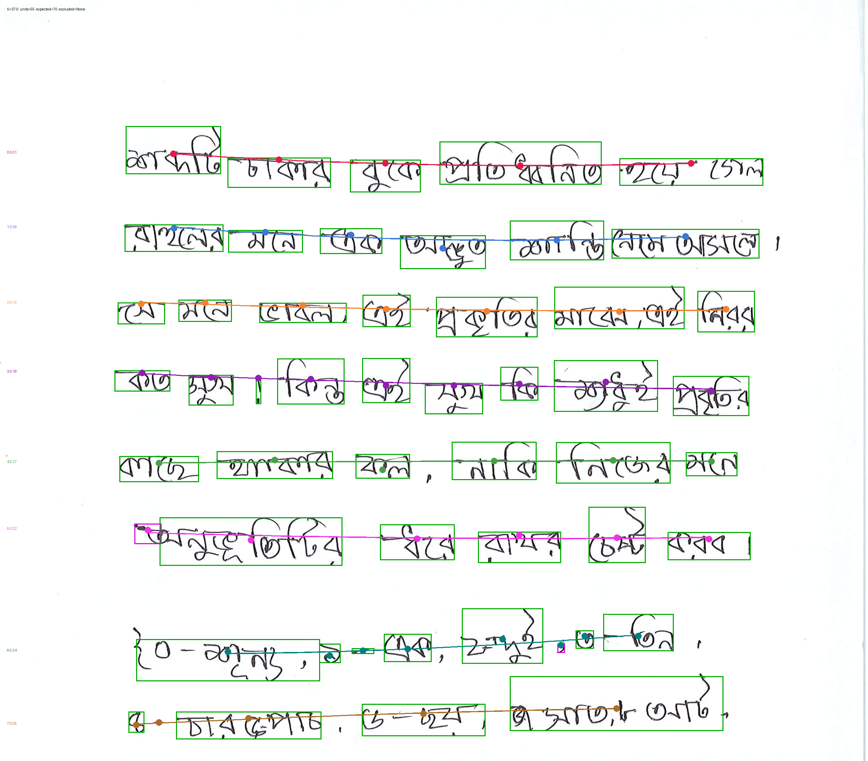
\includegraphics[width=0.48\linewidth]{q_layout_geom.png}
\caption{Extracted geometry on a real page (v1 report): word anchors, fitted line trajectories and residuals.}
\src{\fp{scribe_layout/report/fig/image_103_geom.png}}
\end{figure}

\paragraph{v2 harness and the move to ``unfit'' targets.} v2 (\fp{scribe_layout_v2/}) re-evaluates v1 on a stricter harness
with more C2ST features: there, v1's line C2ST is $0.566\pm0.021$. Table~\ref{tab:v2steps} gives the sequence of v2 models.
The first v2 models (\texttt{v2\_history}, \texttt{v2\_latent}) learned the \emph{fitted} wobble. Fitting a quadratic to
$n$ points shrinks the residuals (``fit shrinkage''), and replaying them adds a second fit at measurement. Training on
inflated (``unfit'') targets lowered the line C2ST from 0.638 to 0.539 (single seed then 5 seeds).

\paragraph{A bug in the unfit targets, and the fix.} A review (M2) found that the inflation table matched the \emph{line}
robust scale but was also applied to every per-word residual. This made per-word wobble overshoot: in a simulation with
i.i.d.\ wobble of sd 0.150, the old table recovers 0.311 at $n=5$, while per-word leverage correction recovers 0.142. The
2-D FFT C2ST had already flagged this. Scaling the drawn wobble moved it from 0.683 ($\times1.0$) to 0.578 ($\times0.5$)
(3 seeds). The leverage fix \texttt{unfitw} gave the best line C2ST, $0.521\pm0.019$.

\paragraph{Curvature deconvolution (the default).} In end-to-end runs the real detector split 89 of 462 drawn v2 lines (19\%),
against 6 of 355 (1.7\%) for manual. At the split points, adjacent words stepped by a median 1.2\U, more than the chainer's
1.0\U{} join threshold. The cause was lines that bow too much. Curvature is sampled before the word count is known, and
fitted $c_2$ on 5--6-word lines is mostly noise (measured sd 0.00129, noise 0.00092, implied true 0.00091). An
extreme-deconvolution likelihood removes this: sampled sag matches real ($|$sag$|>0.5$\U{} on 9.3\% of lines, real 10.8\%,
\texttt{unfitw} 17.5\%), and end-to-end splitting halves to 52/469 (11.1\%). Its C2ST is within noise of \texttt{unfitw}.
\texttt{unfitw\_dc} was chosen for realism, not for C2ST.

\paragraph{A rejected variant.} A Huber-aware per-word correction (\texttt{unfitwh\_dc}) is exact for i.i.d.\ wobble, but was
worse on all three C2STs on both splits (6/6 comparisons). Real wobble is smoother than i.i.d.\ (lag-1 $-0.38$ vs $-0.48$),
so the larger edge inflation overshoots.

\begin{table}[H]
\centering
\caption{Plan-level C2ST AUC by model, TEST (193 pages), 5 seeds, mean $\pm$ sd. Resid-scale W1 is given by words per
line.}
\label{tab:v2steps}
\small
\begin{tabular}{@{}lcccc@{}}
\toprule
model & line C2ST & page C2ST & 2-D FFT C2ST & resid\_scale W1, $n$=5 / 6--7 / 8--10 / 11+ \\
\midrule
manual (BengaliScribe) & 0.980 & 1.0 & 0.99 & -- \\
v1 & $0.566\pm0.021$ & $0.654\pm0.043$ & $0.567\pm0.034$ & .011 / .025 / .055 / .074 \\
v2\_history (1 seed) & 0.638 & 0.752 & -- & -- \\
v2\_history\_unfit (old table) & $0.539\pm0.016$ & $0.660\pm0.004$ & $0.653\pm0.024$ & .039 / .028 / .029 / .058 \\
v2 unfitw (leverage) & $\mathbf{0.521\pm0.019}$ & $\mathbf{0.581\pm0.026}$ & $0.566\pm0.025$ & .009 / .011 / .041 / .062 \\
\textbf{v2 unfitw\_dc (default)} & $0.535\pm0.012$ & $0.590\pm0.024$ & $0.550\pm0.020$ & .007 / .011 / .042 / .061 \\
v2 unfitwh\_dc (Huber, rejected) & $0.544\pm0.012$ & $0.614\pm0.011$ & $0.583\pm0.029$ & .009 / .014 / .043 / .068 \\
shuffled real (not a floor) & $0.584\pm0.016$ & $0.605\pm0.012$ & $0.529\pm0.050$ & .021 / .018 / .054 / .100 \\
within-page null & $0.496\pm0.019$ & -- & -- & -- \\
\bottomrule
\end{tabular}
\src{\fp{scribe_layout_v2/runs/compare_unfitw/compare_5seed.txt}, \fp{compare_5seed_dc.txt}, \fp{compare_5seed_wh_test.txt};
v2\_history row: \fp{scribe_layout_v2/runs/eval/metrics.json}; null and manual: \fp{scribe_layout_v2/report/FACTS.md}}
\end{table}

\paragraph{Selection-free VAL check.}
\label{sec:layoutval}
Every choice above was made on TEST, so the TEST numbers are optimistic. Table~\ref{tab:v2val} repeats the comparison on VAL.
The leverage-family models beat v1 on line and page C2ST on VAL too. The old-table \texttt{unfit} model, which looked better
than v1 on TEST (0.539), is not better on VAL (0.566 vs 0.560): that earlier claim was a selection effect.

\begin{table}[H]
\centering
\caption{Plan-level C2ST on the VAL split (4 texts), 5 seeds.}
\label{tab:v2val}
\small
\begin{tabular}{@{}lcccc@{}}
\toprule
model & line C2ST & page C2ST & FFT C2ST & resid\_scale W1 by $n$ \\
\midrule
v1 & $0.560\pm0.024$ & $0.631\pm0.040$ & $0.531\pm0.033$ & .013 / .025 / .055 / .089 \\
v2 unfit (old table) & $0.566\pm0.028$ & $0.660\pm0.022$ & $0.599\pm0.051$ & .049 / .030 / .024 / .050 \\
v2 unfitw & $0.527\pm0.030$ & $0.575\pm0.039$ & $0.528\pm0.024$ & .012 / .011 / .035 / .072 \\
\textbf{v2 unfitw\_dc (default)} & $0.536\pm0.027$ & $0.593\pm0.031$ & $0.535\pm0.044$ & .011 / .011 / .035 / .069 \\
v2 unfitwh\_dc & $0.551\pm0.022$ & $0.619\pm0.043$ & $0.551\pm0.049$ & -- \\
shuffled real & $0.577\pm0.023$ & $0.597\pm0.030$ & $0.480\pm0.034$ & .016 / .017 / .055 / .089 \\
\bottomrule
\end{tabular}
\src{\fp{scribe_layout_v2/runs/compare_unfitw/compare_5seed_val.txt}, \fp{compare_5seed_wh_val.txt}}
\end{table}

\begin{figure}[H]
\centering
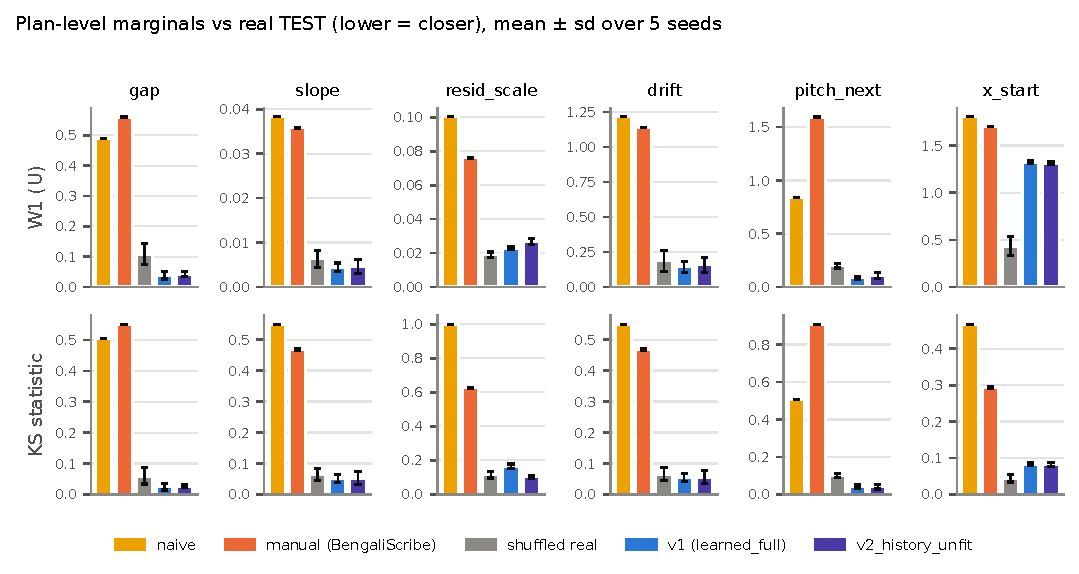
\includegraphics[width=\linewidth]{layout_w1_ks.pdf}
\caption{Plan-level marginals against real TEST on the v2 harness: W1 (top) and KS (bottom). Learned layouts (blue, violet)
match gaps, slope, drift and pitch far better than naive or manual layout. $x_\mathrm{start}$ remains the weakest learned
quantity; shuffled real does better there.}
\src{\fp{scribe_layout_v2/runs/eval/metrics.json} (via \fp{make_figs.py})}
\end{figure}

\begin{figure}[H]
\centering
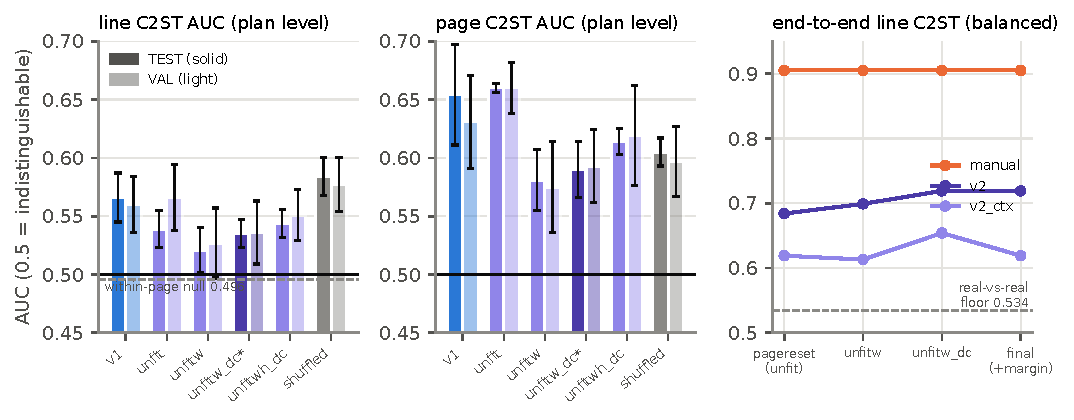
\includegraphics[width=\linewidth]{layout_c2st.pdf}
\caption{C2ST AUC per model. Left and centre: plan level, TEST (solid) and VAL (light), 5 seeds, $\pm$ sd. ``*'' marks the
default. Right: end-to-end line C2ST, balanced protocol only. The two earliest end-to-end runs used a biased C2ST and are
excluded (see text).}
\src{\fp{scribe_layout_v2/runs/compare_unfitw/compare_5seed*.txt}, \fp{scribe_layout_v2/runs/e2e_*/results.md}}
\end{figure}

\paragraph{End-to-end evaluation.} BengaliScribe renders pages for 5 reference writers $\times$ 2 seeds. The real detector
and the same extraction then measure them, and they are compared with the 193 real TEST pages. Variants: \texttt{manual},
\texttt{v2} and \texttt{v2\_ctx} (conditioned on the writer's own real geometry). \textbf{The first two runs
(\texttt{e2e\_unfit}, \texttt{e2e\_unfit\_ink}) used a biased C2ST.} Pooled out-of-fold AUC with one label per page group put
the real-vs-real ``floor'' at 0.34 (line) and 0.115 (page). Their C2ST values are not comparable with later runs; only their
W1 columns are shown. From \texttt{e2e\_pagereset} onward the C2ST is balanced (folds dealt per label; mean of per-fold
AUCs), with floor 0.534 / 0.508.

\begin{table}[H]
\centering
\caption{End-to-end results (W1 in U; AUC). $^{\ddagger}$Biased C2ST: not comparable. Recovered = extracted words /
drawn words.}
\label{tab:e2e}
\small
\begin{tabular}{@{}llccccccc@{}}
\toprule
run (model) & method & gap & slope & drift & pitch & $x_\mathrm{start}$ & line / page C2ST & recovered \\
\midrule
\multirow{2}{*}{e2e\_unfit (canvas-width)} & v2 & 0.602 & 0.015 & 0.531 & 0.716 & 3.837 & \textcolor{gray}{0.750 / 0.901}$^{\ddagger}$ & 0.969 \\
 & v2\_ctx & 0.381 & 0.013 & 0.427 & 0.924 & 4.416 & \textcolor{gray}{0.595 / 0.901}$^{\ddagger}$ & 0.910 \\
\multirow{2}{*}{e2e\_unfit\_ink (ink extents)} & v2 & 0.471 & 0.016 & 0.503 & 0.712 & 4.037 & \textcolor{gray}{0.667 / 0.840}$^{\ddagger}$ & 0.952 \\
 & v2\_ctx & 0.207 & 0.010 & 0.343 & 1.001 & 4.438 & \textcolor{gray}{0.532 / 0.918}$^{\ddagger}$ & 0.866 \\
\midrule
all balanced runs & manual & 0.685 & 0.035 & 0.965 & 1.839 & 0.948 & 0.905 / 0.999 & 1.004 \\
\multirow{2}{*}{e2e\_pagereset (unfit)} & v2 & 0.404 & 0.013 & 0.396 & 0.670 & 4.065 & 0.684 / 0.834 & 0.965 \\
 & v2\_ctx & 0.267 & 0.017 & 0.558 & 0.770 & 3.783 & 0.619 / 0.889 & 0.926 \\
\multirow{2}{*}{e2e\_unfitw} & v2 & 0.376 & 0.012 & 0.343 & 0.346 & 2.278 & 0.699 / 0.851 & 0.960 \\
 & v2\_ctx & 0.197 & 0.019 & 0.610 & 0.480 & 2.703 & 0.613 / 0.842 & 0.933 \\
\multirow{2}{*}{e2e\_unfitw\_dc} & v2 & 0.387 & 0.021 & 0.645 & 0.465 & 1.453 & 0.719 / 0.844 & 0.983 \\
 & v2\_ctx & 0.183 & 0.023 & 0.695 & 0.535 & 2.494 & 0.654 / 0.847 & 0.929 \\
\multirow{2}{*}{\textbf{e2e\_final} (default + margin guard)} & v2 & 0.425 & 0.021 & 0.672 & 0.390 & 1.239 & 0.719 / 0.850 & 0.981 \\
 & v2\_ctx & 0.198 & 0.020 & 0.621 & 0.503 & 2.130 & 0.619 / 0.845 & 0.940 \\
\bottomrule
\end{tabular}
\src{\fp{scribe_layout_v2/runs/e2e_{unfit,unfit_ink,pagereset,unfitw,unfitw_dc,final}/results.md}}
\end{table}

Reading the end-to-end numbers:
\begin{itemize}
\item \textbf{The planner reset was a real fix.} The history used to run across pages, reaching 56--72 lines against at most
  16 in training. Slopes random-walked to the $-0.2$ clamp and words were drawn past the page bottom. After the reset, page
  slope means stay near the writer's (e.g.\ image\_104 with context: $-0.053\dots-0.009$ against real $-0.023$).
\item \textbf{Slope and drift W1 are not comparable across runs with different split rates} (survivor bias). Split lines
  are the steep and bowed ones. In \texttt{e2e\_unfitw}, kept lines had median $|$slope$|$ 0.026 against 0.046 for split
  lines. All drawn \texttt{dc} lines have median $|$slope$|$ 0.027 (q90 0.071), against real 0.029 (0.086).
\item \textbf{Placement bias.} Ink extents use \texttt{INK\_LEVEL} 0.35 while page Otsu is $\approx$0.39, which leaves a
  $+0.067$\U{} bias in every measured gap.
\item \textbf{Line splitting.} With 57 of 453 drawn lines split (12.6\%) in \texttt{e2e\_final}, end-to-end metrics see
  only the surviving lines, and the large $x_\mathrm{start}$ W1 mostly comes from fragments that start mid-page.
\end{itemize}

\begin{figure}[H]
\centering
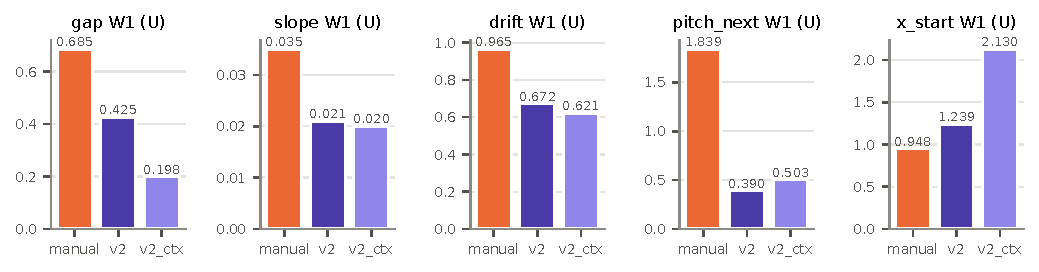
\includegraphics[width=\linewidth]{layout_e2e_final_w1.pdf}
\caption{End-to-end W1 to real TEST for the final run (\texttt{e2e\_final}).}
\src{\fp{scribe_layout_v2/runs/e2e_final/results.md}}
\end{figure}

\begin{figure}[H]
\centering
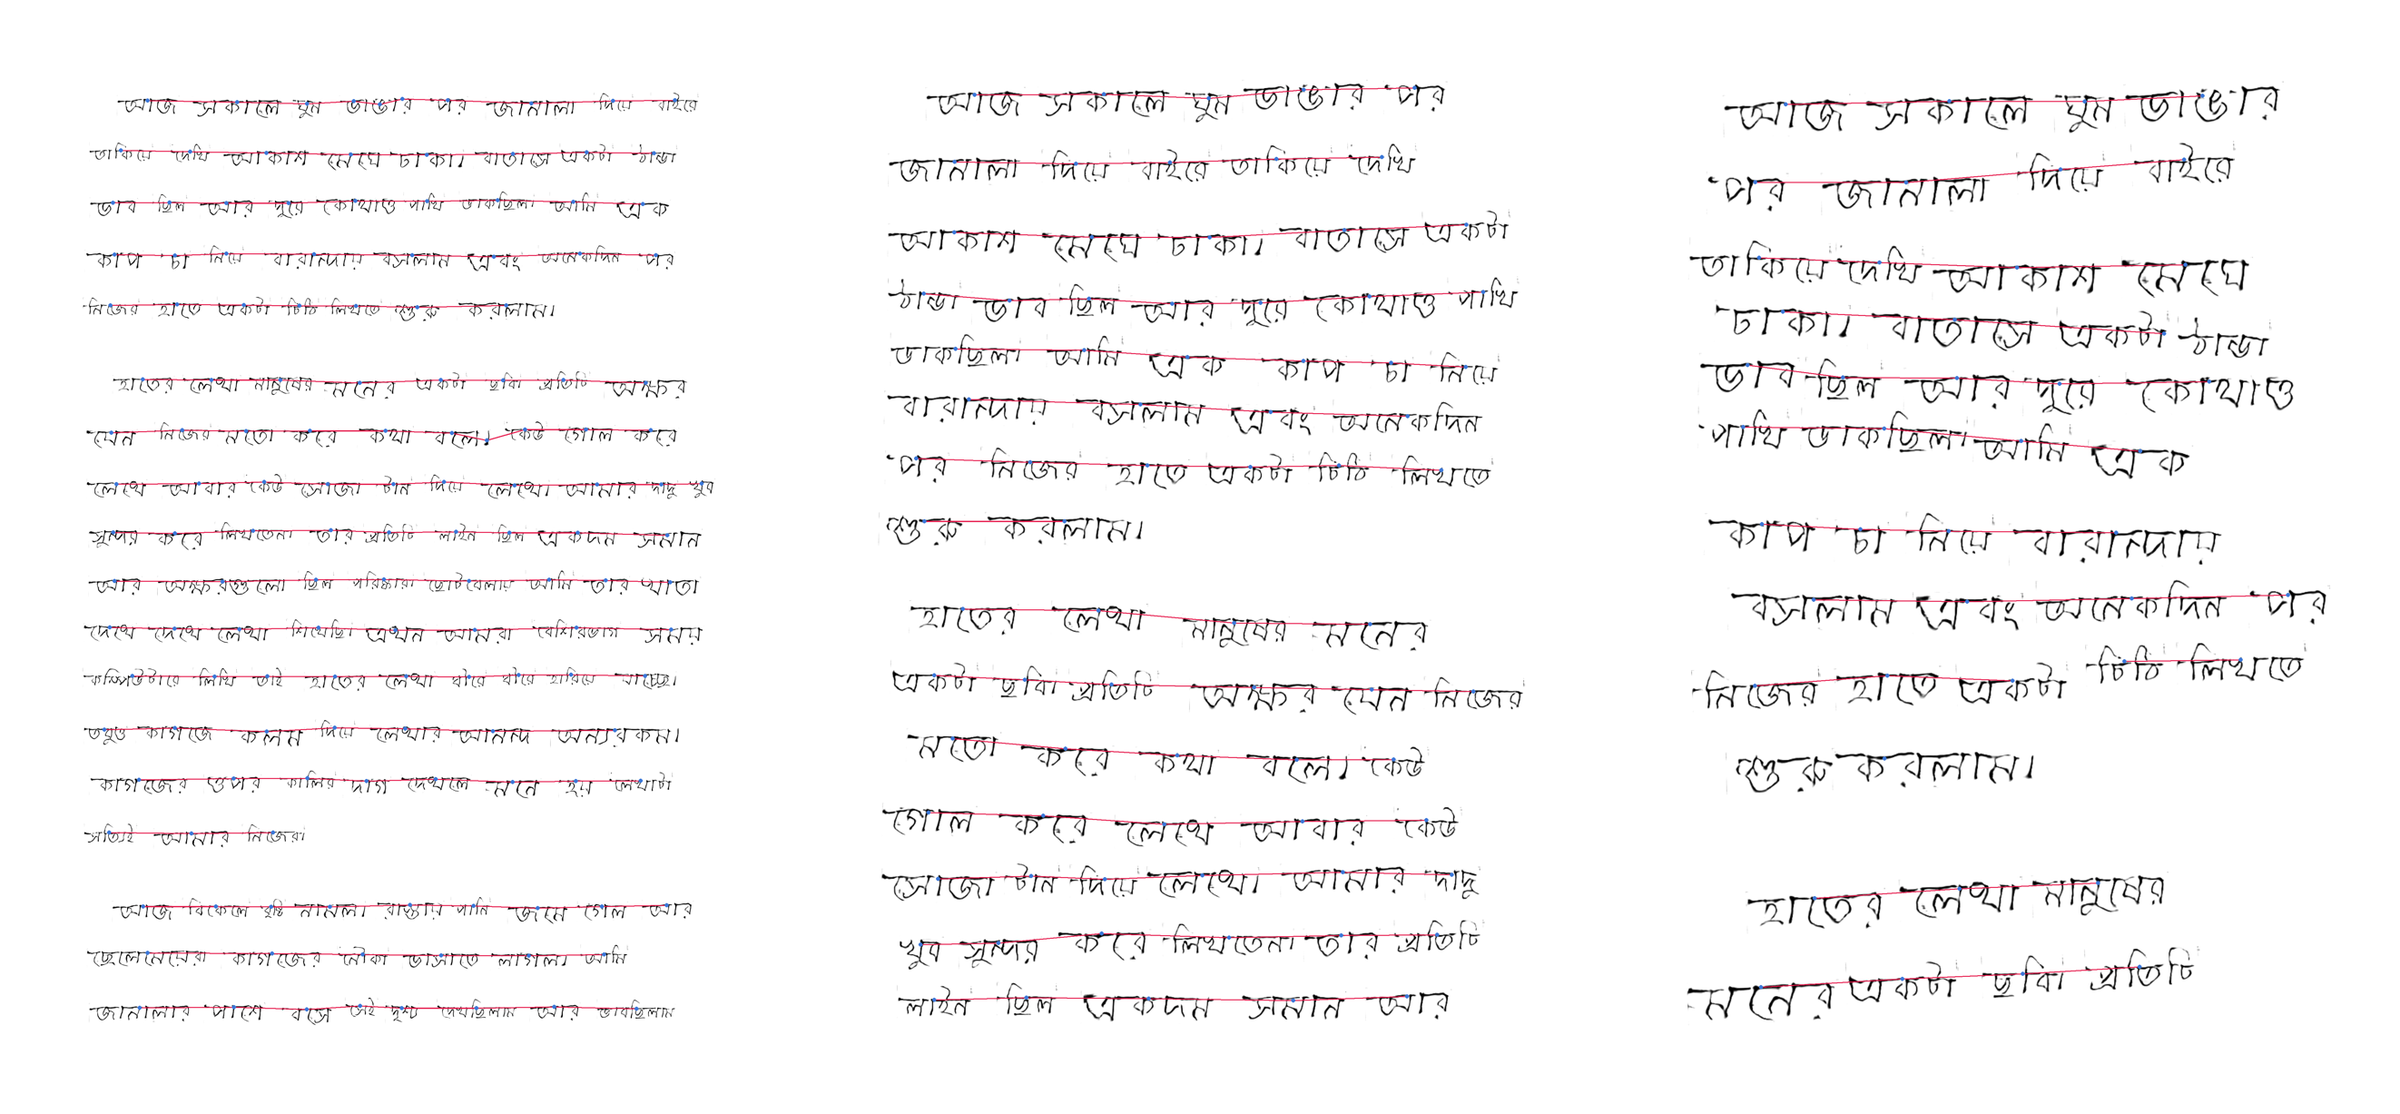
\includegraphics[width=\linewidth]{q_layout_thumbs.png}
\caption{\texttt{e2e\_final} pages for reference writer image\_104 (BengaliScribe B0 words): manual layout (left), v2 (centre),
v2 with writer context (right).}
\src{\fp{scribe_layout_v2/runs/e2e_final/thumbs/image_104_{manual,v2,v2_ctx}.png}}
\end{figure}

\paragraph{Final default model.} \fp{scribe_layout_v2/runs/default_unfitw_dc/model.pt} is the default of
\fp{bscribe_run.py} and \fp{relayout.py}. It runs with the margin guard: a line whose ink would cross the bottom margin starts
a new page and is replanned from scratch. A test asserts that ink stays within the margins $\pm0.5$\U; it fails on the old
code. The layout test suite grew from 32 tests ($\approx$8\,min) to 70 ($\approx$17\,s). The latent writer-style variant is
\textbf{not} the default: a context bug fix (causal-prefix $z$) improved the context case but regressed the no-context model
(page C2ST 0.684 $\to$ 0.829), and the issue is unresolved.

\subsection{Spectral side-studies, with corrections}
\label{sec:spectral}

\paragraph{2-D FFT layout-realism metric (\fp{scribe_layout_fft2d/}).} A layout map is the filled word boxes at 8\,px/U,
Hann-windowed. Its 2-D power spectrum is summarised as radial PSD (32 bins), angular energy (18 bins) and the vertical
line-pitch peak. \textbf{Only the controlled (text-matched) comparison is valid.} The uncontrolled version is confounded:
single non-layout features alone separate real from generated (text-block height AUC 0.985, median word width 0.90--0.93),
so its AUCs of 0.96--1.0 measured text, page fill and glyphs, not layout. In the controlled test every generator runs on each
real page's own word widths, both sides use the same fixed box, and confound AUCs are 0.5 by construction.

\begin{figure}[H]
\centering
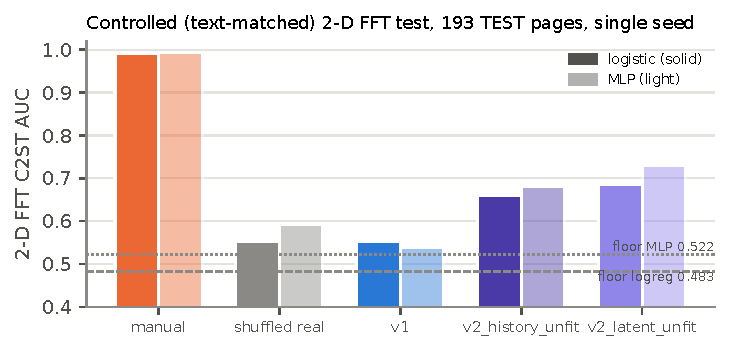
\includegraphics[width=0.78\linewidth]{spectral_fft2d_controlled.pdf}
\caption{Controlled 2-D FFT C2ST, single seed. Single-seed AUCs move by up to $\pm0.09$; the 5-seed FFT C2STs are in
Table~\ref{tab:v2steps}. Pitch ablations on real pages show that the spectrum is dominated by line-pitch regularity.
Shuffling pitch moves the mean log-PSD 6$\times$ more (L2 0.080) than zeroing slope (0.013) or removing wobble (0.013).}
\src{\fp{scribe_layout_fft2d/runs/results.md} (controlled section only), \fp{scribe_layout_v2/report/FACTS.md}}
\end{figure}

\begin{figure}[H]
\centering
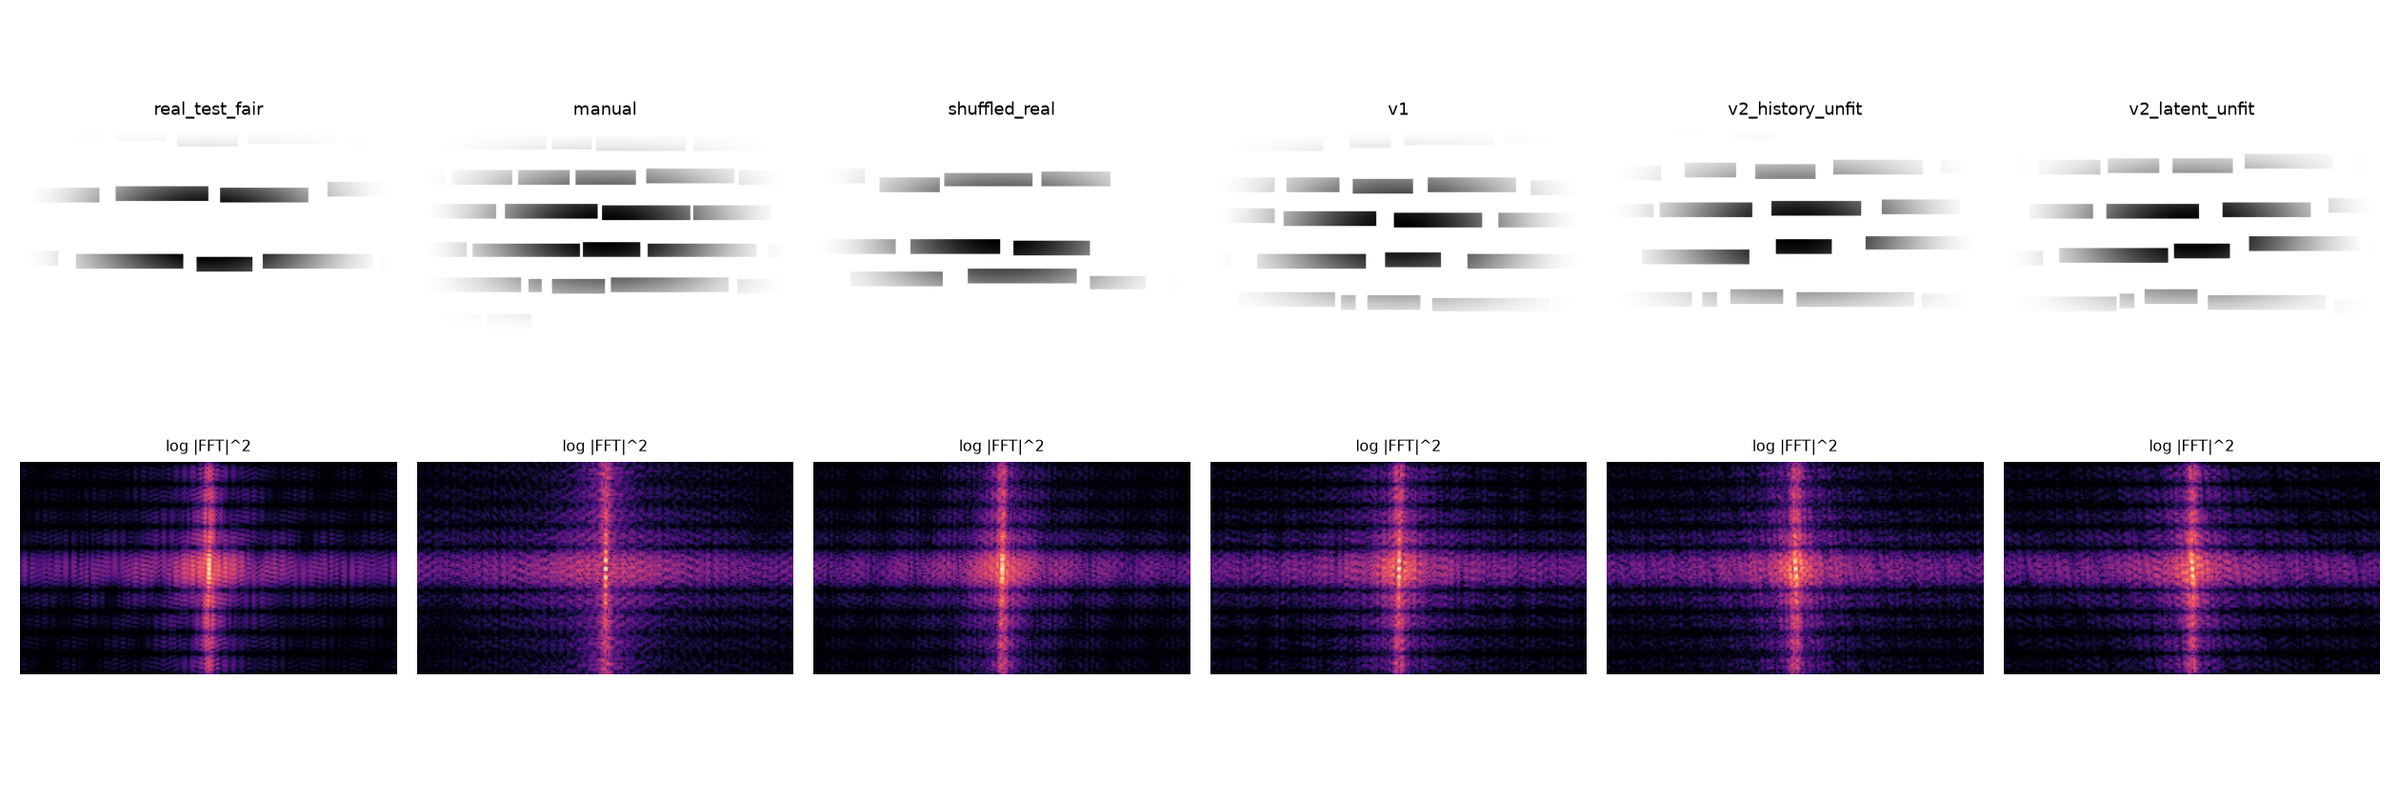
\includegraphics[width=\linewidth]{q_fft_layout_maps.png}
\caption{Controlled layout maps (fixed word boxes) used by the 2-D FFT metric: real page and generated layouts on the same
word widths.}
\src{\fp{scribe_layout_v2/report/figs/example_layout_maps_fair.png}}
\end{figure}

\paragraph{1-D Fourier model of the headline (\fp{scribe_layout_fourier/}).} Dense headline traces of real lines follow a
power law, PSD $\propto f^{-\alpha}$ with $\alpha=1.06$ ($R^2=0.99$, 5,099 train lines), with no word-period peak. A
spectral-synthesis generator samples Gaussian-process headlines with this spectrum. Its \fp{runs/results.md} states that
Fourier is ``17$\times$ better'' than v1 (log-spectral RMSE 3.98 vs 0.23 nats). \textbf{That claim is wrong.} The 0.23
belongs to a continuous trace that no layout of rigid words can draw. v1's 3.98 is a floor artefact, because the comparison
ran on traces that a layout cannot realise. The corrected, fair comparison uses layout-realisable traces (rigid, rotated
words) and the band with wavelength $\ge$4\U. The distance to real is then: manual 3.786, \textbf{v1 0.702, Fourier 0.668},
continuous Fourier (not realisable) 0.244. \textbf{Fourier and v1 are essentially equal.} The ``6$\times$ better
$x_\mathrm{start}$'' claim from the same study came from including indents.

\begin{figure}[H]
\centering
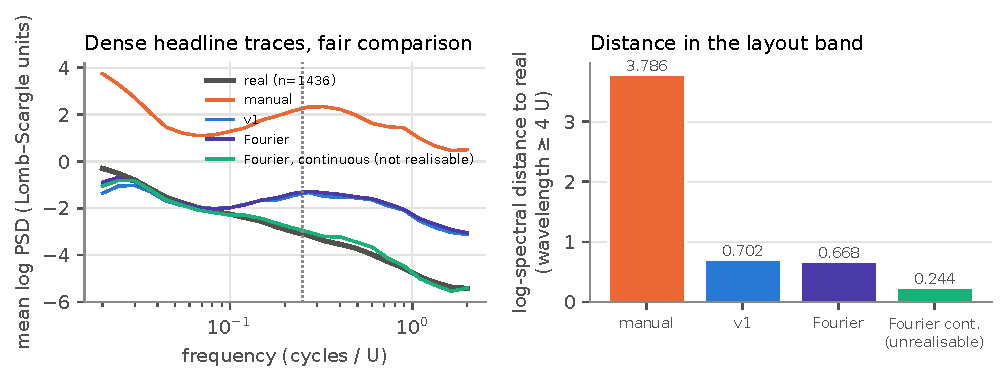
\includegraphics[width=\linewidth]{spectral_fourier_fair.pdf}
\caption{Corrected Fourier comparison. Left: mean log PSD of dense headline traces (dotted line: the 4\U{} wavelength
limit). Right: log-spectral distance to real in the layout band.}
\src{\fp{scribe_layout_fourier/runs/fair_dense_psd.json}; correction in \fp{scribe_layout_v2/report/FACTS.md}}
\end{figure}

%=============================================================================
\section{Word generation}
\label{sec:wordgen}

\subsection{From diagnosis to design}
The diagnosis (\S\ref{sec:intro}) implies that a higher-resolution B0 would still copy the font: construction has to be
learned from the references by a model that is not tied to a font raster. The primary approach is a \textbf{few-shot latent
diffusion word generator} built from DiffusionPen: an SD-1.5 VAE, a U-Net with CANINE text cross-attention, and a style
vector from 5 references. Candidates are re-adapted from the IAM checkpoint on TRAIN writers only. \texttt{dp\_words\_b64},
which saw every BW writer, is used only as a probe and a baseline (B3). Table~\ref{tab:armlist} lists the arms.

\begin{table}[H]
\centering
\caption{Generator arms.}
\label{tab:armlist}
\small
\begin{tabular}{@{}lp{12.6cm}@{}}
\toprule
arm & definition \\
\midrule
B0 & BengaliScribe font-prior GAN (NotoSans prior), \texttt{models/v2} \\
B3 & \texttt{dp\_words\_b64}: DiffusionPen fine-tuned on all 260 BW writers (fair only on BN-HTR) \\
A, B (P1a) & DiffusionPen from IAM on TRAIN, 40 crops/writer cap, 20k steps; B adds an 8-ch painted grapheme content map \\
\Ap, \Bp{} (P1a$'$) & full TRAIN (98,856 crops, 354 writers), white-paper normalisation, 40k steps; \Bp{} adds grapheme tokens + column-position encodings in cross-attention \\
\Bp{}v2 & \Bp{} sampled with \texttt{fit\_canvas\_white2} (bgnorm2) references, no retraining \\
P & \Bp{} + pen knob (scalar embedding of the refs' $\log$ width/core) + learned null style + rebalanced sampling; 16k steps \\
S & P + 16 reference tokens per ref (Bengali SupCon ResNet-18) in decoupled (IP-Adapter-style) cross-attention; 24k steps \\
\_tXcY / \_cal & text guidance X and content guidance Y; \_cal = page-scale pen calibration (shrink mode) \\
\bottomrule
\end{tabular}
\end{table}

\subsection{probe\_day1: a visible first probe}
\texttt{dp\_words\_b64} was sampled on image\_2's text with three reference sets, and fine-tuned for 120 steps on image\_2's
confident crops. The result was qualitatively the most handwriting-like texture yet: rounder and more flowing than B0
(Fig.~\ref{fig:probe}). But it was not thinner than B0, and it misspelled conjuncts and long words (Table~\ref{tab:probe}).

\begin{table}[H]
\centering
\caption{probe\_day1 (24 image\_2 words; locator CER, mean). Real CER is circular: the ``confident'' crops were selected by
the same locator. Indicative only.}
\label{tab:probe}
\small
\begin{tabular}{@{}lcccc@{}}
\toprule
method & $n$ & width/core (median) & darkness (median) & locator CER \\
\midrule
real (confident crops) & 9 & 0.064 & 1.00 & 0.00 (circular) \\
B0 & 24 & 0.063 & 0.97 & 0.184 \\
DP, image\_2 refs & 24 & 0.091 & 1.00 & 0.973 \\
DP, writer\_99 refs & 24 & 0.110 & 1.00 & 0.931 \\
DP, writer\_117 refs & 24 & 0.104 & 1.00 & 0.899 \\
DP, fine-tuned on image\_2 & 24 & 0.100 & 1.00 & 0.651 \\
\bottomrule
\end{tabular}
\src{\fp{scribe_wordgen/runs/probe_day1/REPORT.md} (``Numbers'')}
\end{table}

\begin{figure}[H]
\centering
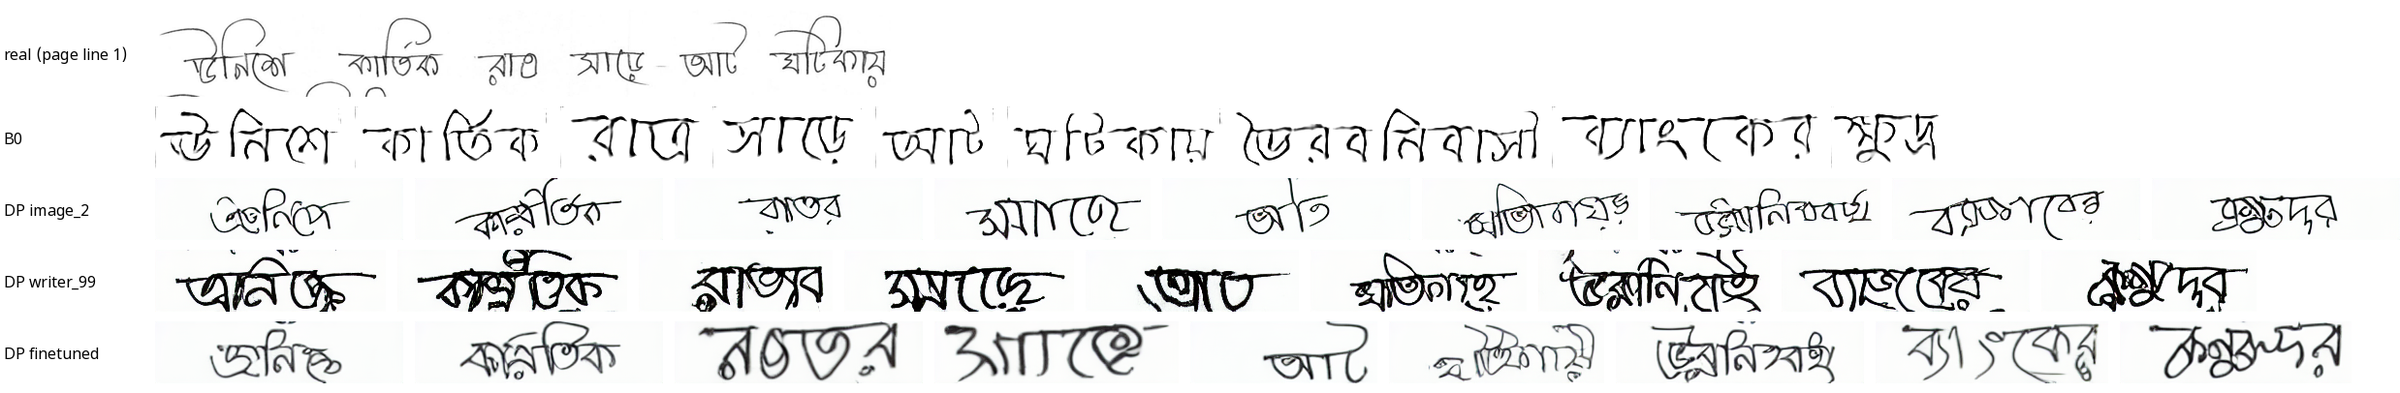
\includegraphics[width=\linewidth]{q_probe_line.png}
\caption{probe\_day1: the first line of image\_2, rendered by different methods (real, B0 and DiffusionPen variants).}
\label{fig:probe}
\src{\fp{scribe_wordgen/runs/probe_day1/line.png}}
\end{figure}

\subsection{P1a: the painted content map is inert (NO-GO)}
P1a trained DiffusionPen from IAM on TRAIN writers (40 crops/writer: 14,155 crops, 5,033 unique texts), 20k steps at
batch 32. Arm A is the text-only control; arm B adds an 8-channel grapheme content map with a zero-initialised first-conv
slice. The review first corrected the metric. Raw CER $>1$ and width/core $\approx4$ were artefacts of uncapped CER on
punctuation, grey-box output on grey-paper writer 117, and truncation of B0 at 256\,px. Table~\ref{tab:p1a} gives the
corrected numbers.

\begin{table}[H]
\centering
\caption{P1a, corrected (VAL, 20 writers; CER capped at 1, left-aligned, punctuation excluded).}
\label{tab:p1a}
\small
\begin{tabular}{@{}lccccc@{}}
\toprule
method & CER & BN-HTR excl.\ 117 & BW & bg-fail \% & sub-px width / real \\
\midrule
real & 0.133 \ci{0.101}{0.169} & 0.049 & 0.237 & 1.2 & 1.00 \\
B0 & 0.130 \ci{0.105}{0.157} & 0.084 & 0.224 & 0.2 & $\approx$1.3 \\
B3 & 0.422 \ci{0.384}{0.460} & 0.427 & 0.476 (optimistic) & 3.8 & 1.32 \\
A & 0.482 \ci{0.440}{0.528} & 0.423 & 0.525 & 8.7 & 1.40 \\
B & 0.457 \ci{0.417}{0.501} & 0.361 & 0.516 & 8.8 & 1.40 \\
\bottomrule
\end{tabular}
\par\smallskip\footnotesize Paired B$-$A $=-0.024$ \ci{-0.045}{-0.002} (14/20 writers), entirely in-vocabulary (OOV: A 0.568, B 0.574).
\src{\fp{scribe_wordgen/runs/P1a/REVIEW.md} \S1}
\end{table}

\textbf{Verdict: NO-GO for the content map.} When another word's map is painted in, the model still writes the CANINE word:
CER against the painted word is 0.959. The map alone gives near-unconditional output (0.953 vs 0.973). The grapheme
embeddings barely moved during training (row norm 0.078 vs init $\approx$0.057). One content patch contributes about 2\% of
the first-conv input signal. The review traced the other failures to grey reference paper (6.4\% of BN-HTR TRAIN crops have
paper $<250$), a starved data set, and a CFG-driven thick pen (arm A: 1.31$\times$ at g1, 1.48$\times$ at g2/g3).

\subsection{P1a$'$: full data, white paper, grapheme tokens and the CFG-null bug}
P1a$'$ applied the review's fixes. It trained on all of TRAIN (98,856 crops) for 40k steps with white-paper normalisation,
and redesigned content as \emph{grapheme-token cross-attention}: learned grapheme embeddings plus column-centre and span
encodings, appended to the CANINE context. The report concluded that \Bp{} was a NO-GO (CER 0.550, worse than \Ap). The
review found the cause.

\paragraph{The CFG-null bug.} \texttt{eval\_v2.sample\_arm2} put the content map and tokens into \emph{both} classifier-free
guidance branches. Guidance therefore extrapolated only the text direction, and content was never guided. The correct null
drops text, map and tokens together, matching the independent 10\% drops used in training. With the joint null (same 781
words, refs and seeds; Table~\ref{tab:p1a2}), \Bp{} becomes the best diffusion arm. The shuffled-content gate passes: the
model writes the \emph{painted} word (CER 0.432 against it at g3). Without any text, content alone writes the word at 0.199.
The content-path ablation shows that the tokens carry identity (tokens alone 0.338), while the painted map is still inert
(map alone 0.902).

\begin{table}[H]
\centering
\caption{P1a$'$ on full VAL with the fixed sampler (eval\_v2 scoring; CER capped at 1, punctuation excluded).}
\label{tab:p1a2}
\small
\begin{tabular}{@{}lccccccc@{}}
\toprule
method & CER all & in-vocab & OOV & BN-HTR & BW & bg-fail & pen (sub-px/core) \\
\midrule
real & 0.133 & 0.129 & 0.150 & 0.055 & 0.159 & 1.2\% & 1.00 \\
B0 & 0.130 & 0.116 & 0.235 & 0.085 & 0.145 & 0.2\% & 1.15 \\
B3 & 0.421 & 0.400 & 0.508 & 0.410 & 0.425 & 3.8\% & 1.13 \\
\Ap{} g2 (as reported) & 0.334 & 0.312 & 0.496 & 0.237 & 0.367 & 5.4\% & 1.36 \\
\Ap{} g3 & 0.245 \ci{0.205}{0.287} & 0.228 & 0.384 & 0.160 & 0.273 & 5.2\% & 1.22 \\
\Bp{} as reported (buggy CFG) & 0.550 & 0.537 & 0.655 & 0.405 & 0.599 & 0.9\% & -- \\
\Bp{} fixed g2 & 0.262 \ci{0.218}{0.304} & 0.239 & 0.385 & 0.153 & 0.298 & 1.3\% & 1.27 \\
\textbf{\Bp{} fixed g3} & \textbf{0.188} \ci{0.150}{0.226} & 0.169 & 0.301 & 0.108 & 0.214 & 1.8\% & 1.29 \\
\Bp{} content only, c4 & 0.199 \ci{0.161}{0.238} & 0.186 & 0.303 & 0.112 & 0.229 & 1.7\% & -- \\
\bottomrule
\end{tabular}
\par\smallskip\footnotesize Paired \Bp{}g3$-$\Ap{}g3 $=-0.057$ \ci{-0.089}{-0.032} (18/20 writers). \Ap{} vs P1a A: $-0.147$
\ci{-0.204}{-0.103} (20/20).
\src{\fp{scribe_wordgen/runs/P1a2/REVIEW.md} \S1--2}
\end{table}

\Ap{} and \Bp{} draw about 1.3$\times$ the writer's pen relative to letter size. That is thicker than B0/B3 (about 1.15),
probably because P1a$'$ training is 84\% BN-HTR, whose pens are thick. Writer 117's faint grey blotches (45--48\% of its words)
were not caught by the bg-fail metric, which motivated the faint-blotch score.

\begin{figure}[H]
\centering
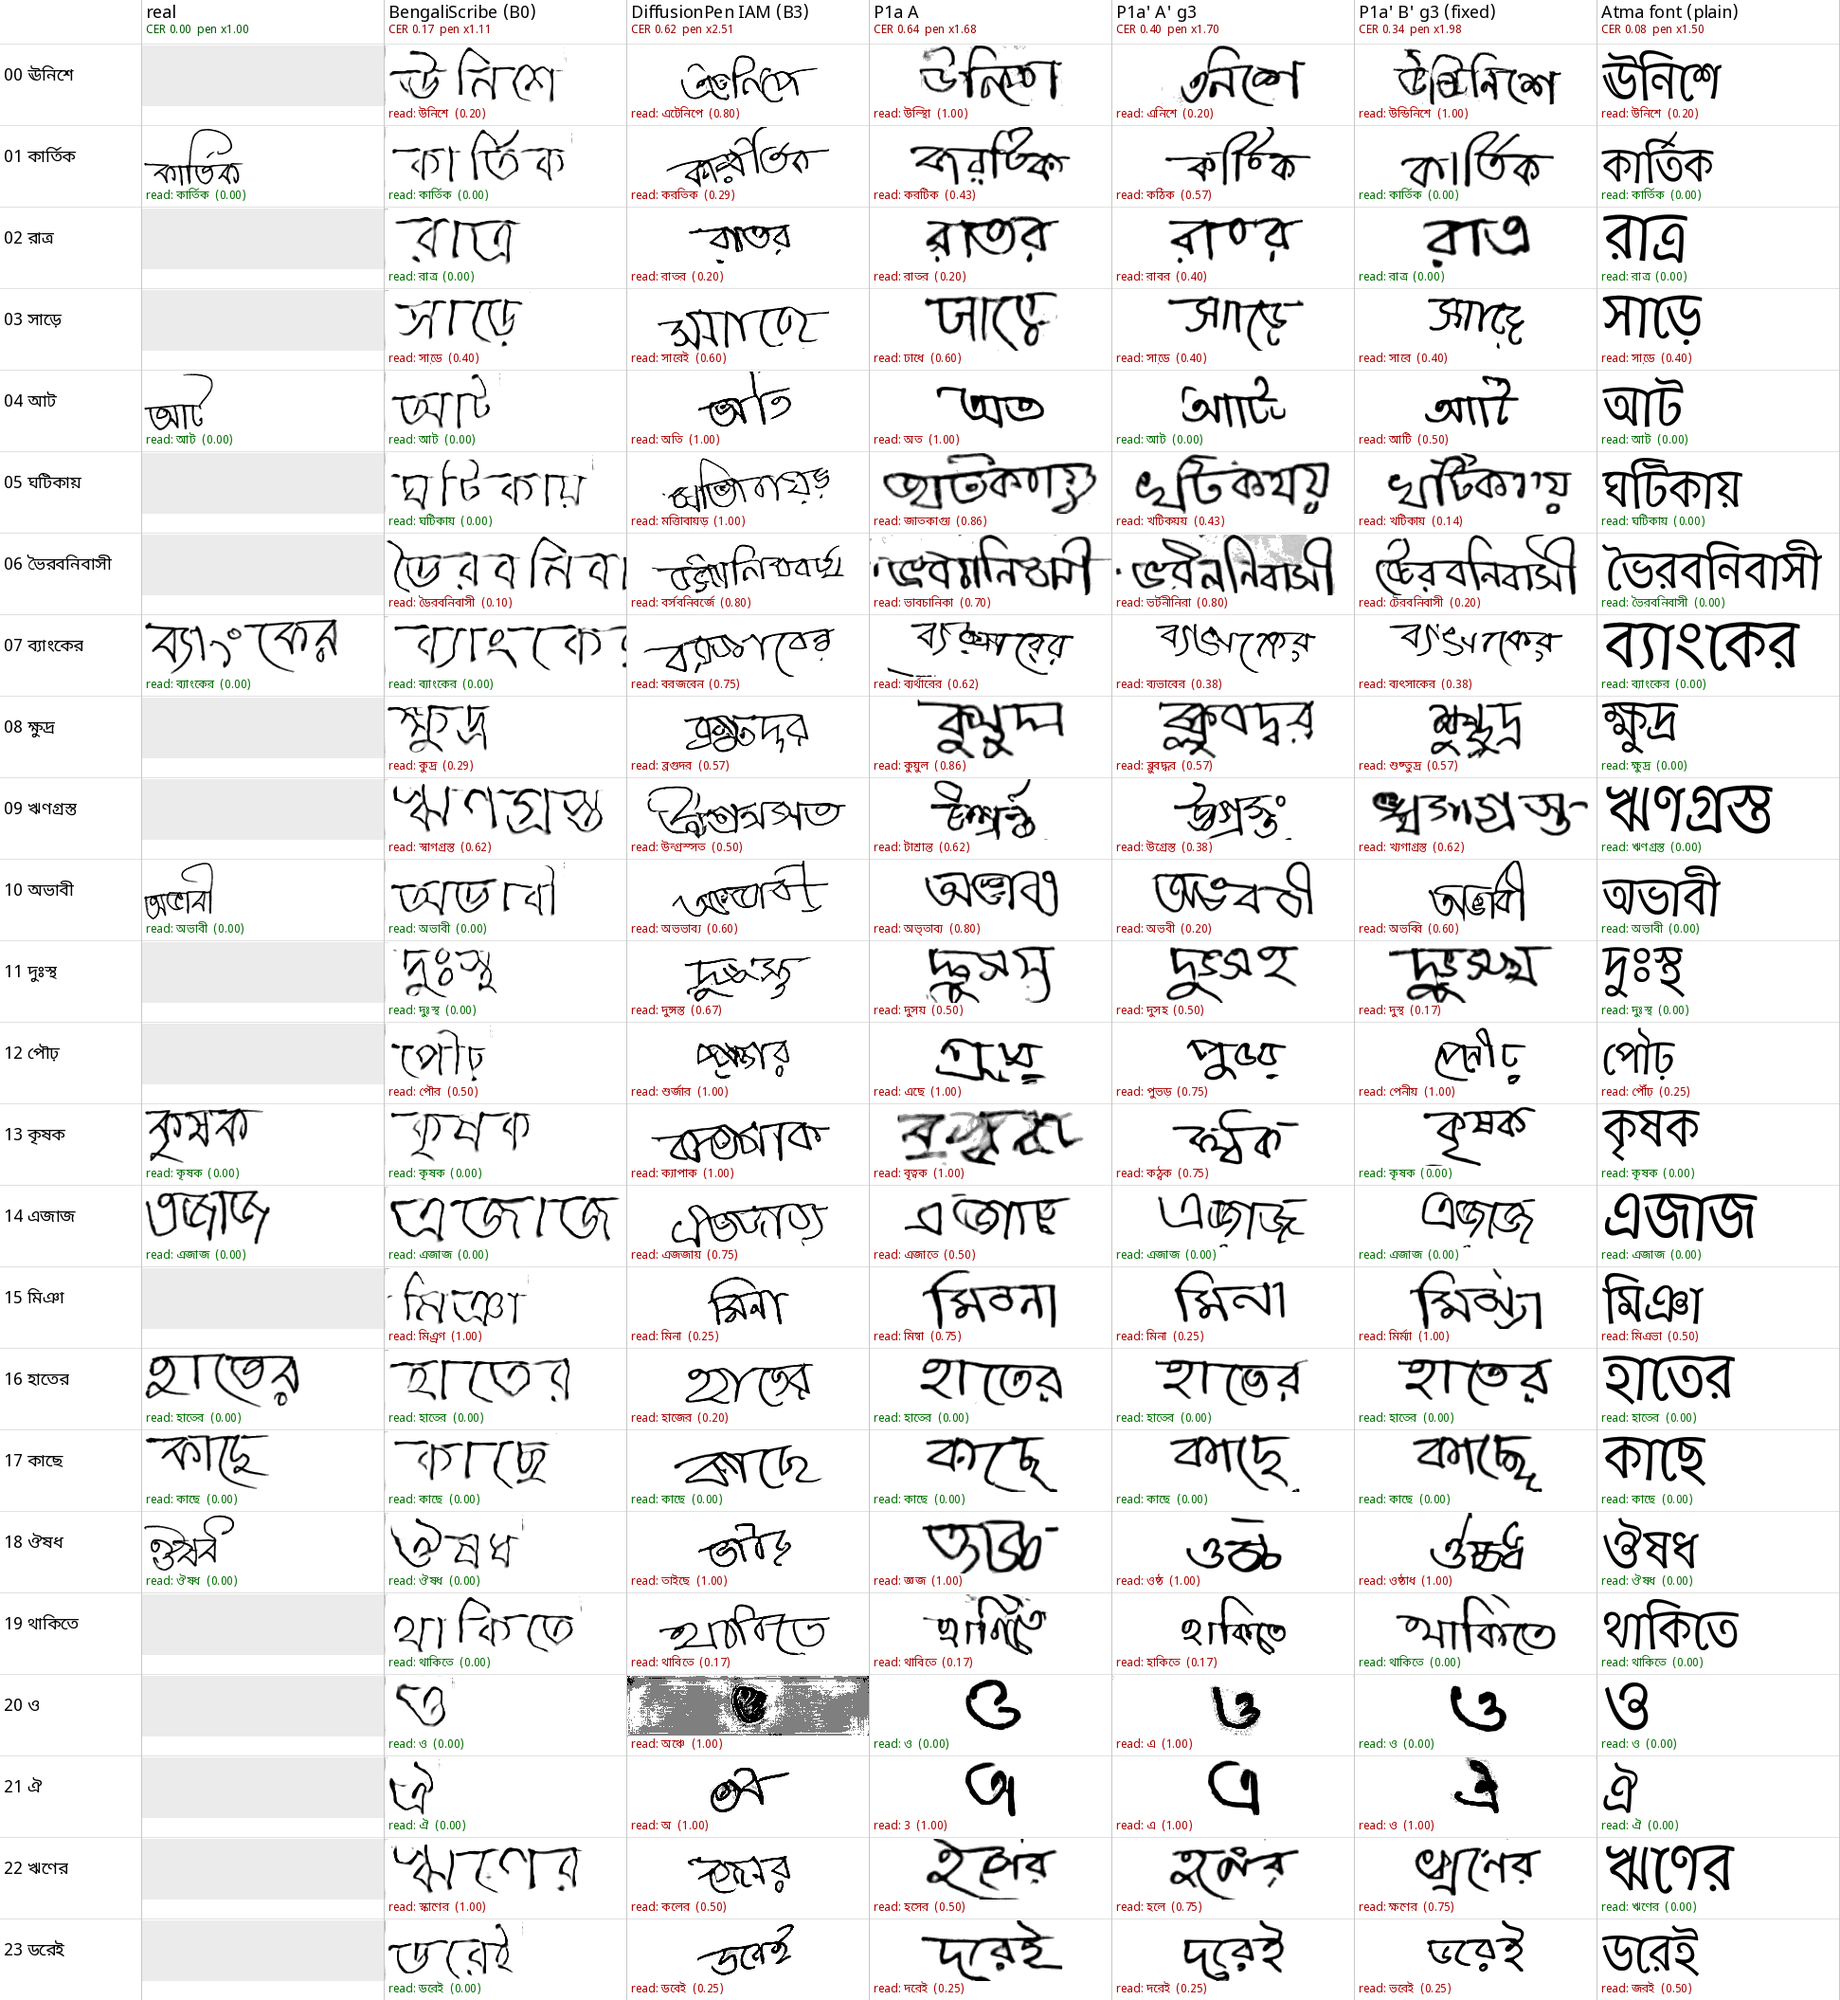
\includegraphics[width=0.92\linewidth]{q_compare_image2.png}
\caption{Side-by-side on image\_2 (24 words, seed 0; the real crop exists for 9 words). Columns: real, B0, B3, P1a A,
P1a$'$ \Ap{} g3, \Bp{} g3 (fixed CFG), plain Atma font. The locator's reading and CER are printed under each cell. image\_2
CER over 3 seeds: B0 0.17, B3 0.62, A 0.64, \Ap{} 0.40, \Bp{} 0.34, Atma 0.08; pen vs writer 1.11 / 2.51 / 1.68 / 1.70 /
1.98 / 1.50.}
\src{\fp{scribe_wordgen/runs/compare_inference/image2_side_by_side.png}, \fp{image2_scores.txt}, \fp{README.md}}
\end{figure}

\subsection{eval\_v3: re-baseline and guidance sweep}
eval\_v3 is the corrected evaluation. It uses the fixed joint CFG null and separate text ($t$) and content ($c$) guidance
scales. The decomposition is $\epsilon=\epsilon_{00}+c\,(\epsilon_{0c}-\epsilon_{00})+t\,(\epsilon_{tc}-\epsilon_{0c})$,
where the subscripts mark which conditioning (text, content) is present. eval\_v3 also adds $\ge$2 seeds per word, the
sub-pixel pen metric, a non-punctuation background gate, the faint-blotch score, and OOV CER on all 20 writers. Seed 0
reproduces the review exactly: \Bp{} t3c3 gives 0.188 with 781/781 pixel-identical renders (\fp{runs/eval_v3/validate.txt}).
Raising guidance lowers CER monotonically to t5c5, which ties B0 (Table~\ref{tab:ev3},
Fig.~\ref{fig:guid}). Pen rises slightly with guidance, and the writer-117 blotch rate falls from 34\% (t2c2) to 11\%
(t5c5).

\begin{table}[H]
\centering
\caption{eval\_v3 guidance sweep for \Bp{} (VAL, 2 seeds; locator CER).}
\label{tab:ev3}
\small
\begin{tabular}{@{}lccccccc@{}}
\toprule
method & CER & in-vocab & OOV (18 wr.) & BN-HTR & BW & pen [CI] & blotch 117 \\
\midrule
real & 0.133 \ci{0.100}{0.167} & 0.129 & 0.150 & 0.055 & 0.159 & 1.00 & 8\% \\
B0 & 0.130 \ci{0.103}{0.156} & 0.116 & 0.235 & 0.085 & 0.145 & 1.15 \ci{0.98}{1.20} & 0\% \\
\Ap{} g3 & 0.254 \ci{0.214}{0.295} & 0.234 & 0.379 & 0.161 & 0.285 & 1.22 & 31\% \\
\Bp{} t2c2 & 0.274 \ci{0.229}{0.317} & 0.255 & 0.393 & 0.143 & 0.318 & 1.26 & 34\% \\
\Bp{} t3c3 & 0.194 \ci{0.156}{0.230} & 0.174 & 0.307 & 0.098 & 0.225 & 1.26 & 21\% \\
\Bp{} t4c4 & 0.165 \ci{0.128}{0.202} & 0.151 & 0.254 & 0.077 & 0.194 & 1.27 & 14\% \\
\Bp{} t5c5 & 0.148 \ci{0.115}{0.182} & 0.133 & 0.241 & 0.068 & 0.175 & 1.30 \ci{1.15}{1.45} & 11\% \\
\Bp{} t6c6 & 0.143 \ci{0.110}{0.178} & 0.126 & 0.247 & 0.064 & 0.170 & 1.31 & 11\% \\
\Bp{} t0c4 (content only) & 0.192 & 0.175 & 0.303 & 0.098 & 0.223 & 1.27 & 18\% \\
\bottomrule
\end{tabular}
\par\smallskip\footnotesize Paired: \Bp{}t5c5$-$B0 $+0.018$ \ci{-0.008}{+0.044} (tie); \Bp{}t6c6$-$\Bp{}t5c5 $-0.005$
\ci{-0.011}{+0.000}; OOV \Bp{}t5c5$-$\Ap{}g3 $-0.138$ \ci{-0.218}{-0.066} (14/18 writers).
\src{\fp{scribe_wordgen/runs/eval_v3/report_tables.txt}}
\end{table}

\begin{figure}[H]
\centering
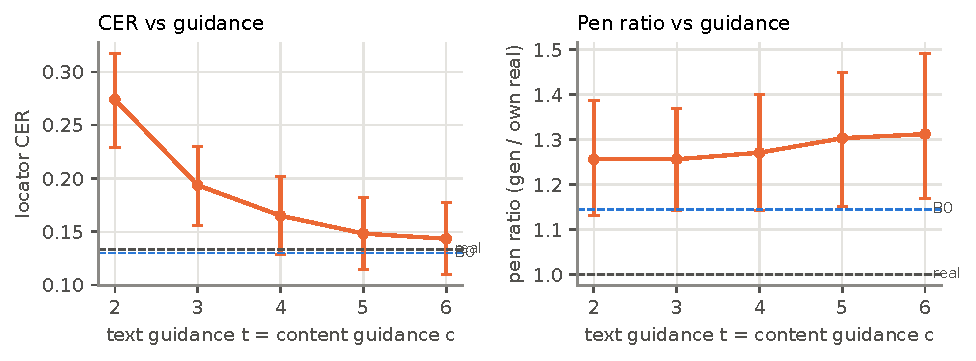
\includegraphics[width=0.95\linewidth]{guidance_sweep.pdf}
\caption{Guidance sweep for \Bp{} with $t=c$. Left: locator CER with writer-bootstrap CI (dashed: real and B0). Right: pen
ratio. More guidance buys legibility, and pen thickens a little.}
\label{fig:guid}
\src{\fp{scribe_wordgen/runs/eval_v3/metrics.json}}
\end{figure}

\subsection{The style evaluator (M2 / M2s)}
Before E\_eval existed, style was judged with the generator's own frozen IAM encoder (real-vs-real MRR 0.41), which is not
independent. E\_eval and E\_shape (\S\ref{sec:eval}) were built and checked before any style claim was made
(Table~\ref{tab:style0}). The first result was sobering: \textbf{every diffusion arm up to \Bp{} sat at MRR 0.40--0.45},
far below B0 (0.596) though above fonts.

\begin{table}[H]
\centering
\caption{Style evaluator validity and early arms (M2, E\_eval, within-dataset galleries, 20 writers / 726 queries).}
\label{tab:style0}
\small
\begin{tabular}{@{}lccc@{}}
\toprule
method & top-1 & MRR & margin \\
\midrule
chance & 0.100 & 0.280 & -- \\
real & 0.723 \ci{0.651}{0.786} & 0.821 \ci{0.775}{0.859} & 0.094 \\
real via \texttt{crop\_ink} & 0.707 & 0.810 & 0.091 \\
B0 & 0.442 \ci{0.310}{0.591} & 0.596 \ci{0.488}{0.711} & $-0.010$ \\
P1a A / P1a B & 0.214 / 0.195 & 0.420 / 0.404 & $-0.133$ / $-0.130$ \\
\Ap{} g3 / \Bp{} g3 & 0.244 / 0.238 & 0.437 / 0.431 & $-0.114$ / $-0.124$ \\
NotoSans font / Atma font & 0.107 / 0.092 & 0.289 / 0.268 & $-0.191$ / $-0.247$ \\
\bottomrule
\end{tabular}
\par\smallskip\footnotesize Paired: real$-$B0 $+0.225$ \ci{+0.116}{+0.335}; \Bp{}g3$-$B0 $-0.165$ \ci{-0.287}{-0.047};
\Bp{}g3$-$Noto $+0.142$ \ci{+0.033}{+0.247}. BN-HTR only: real 0.916, B0 0.883 (real$-$B0 n.s.).
\src{\fp{scribe_wordgen/runs/style_eval/tables.md} (``eval within all'', ``eval within bnhtr'')}
\end{table}

\begin{figure}[H]
\centering
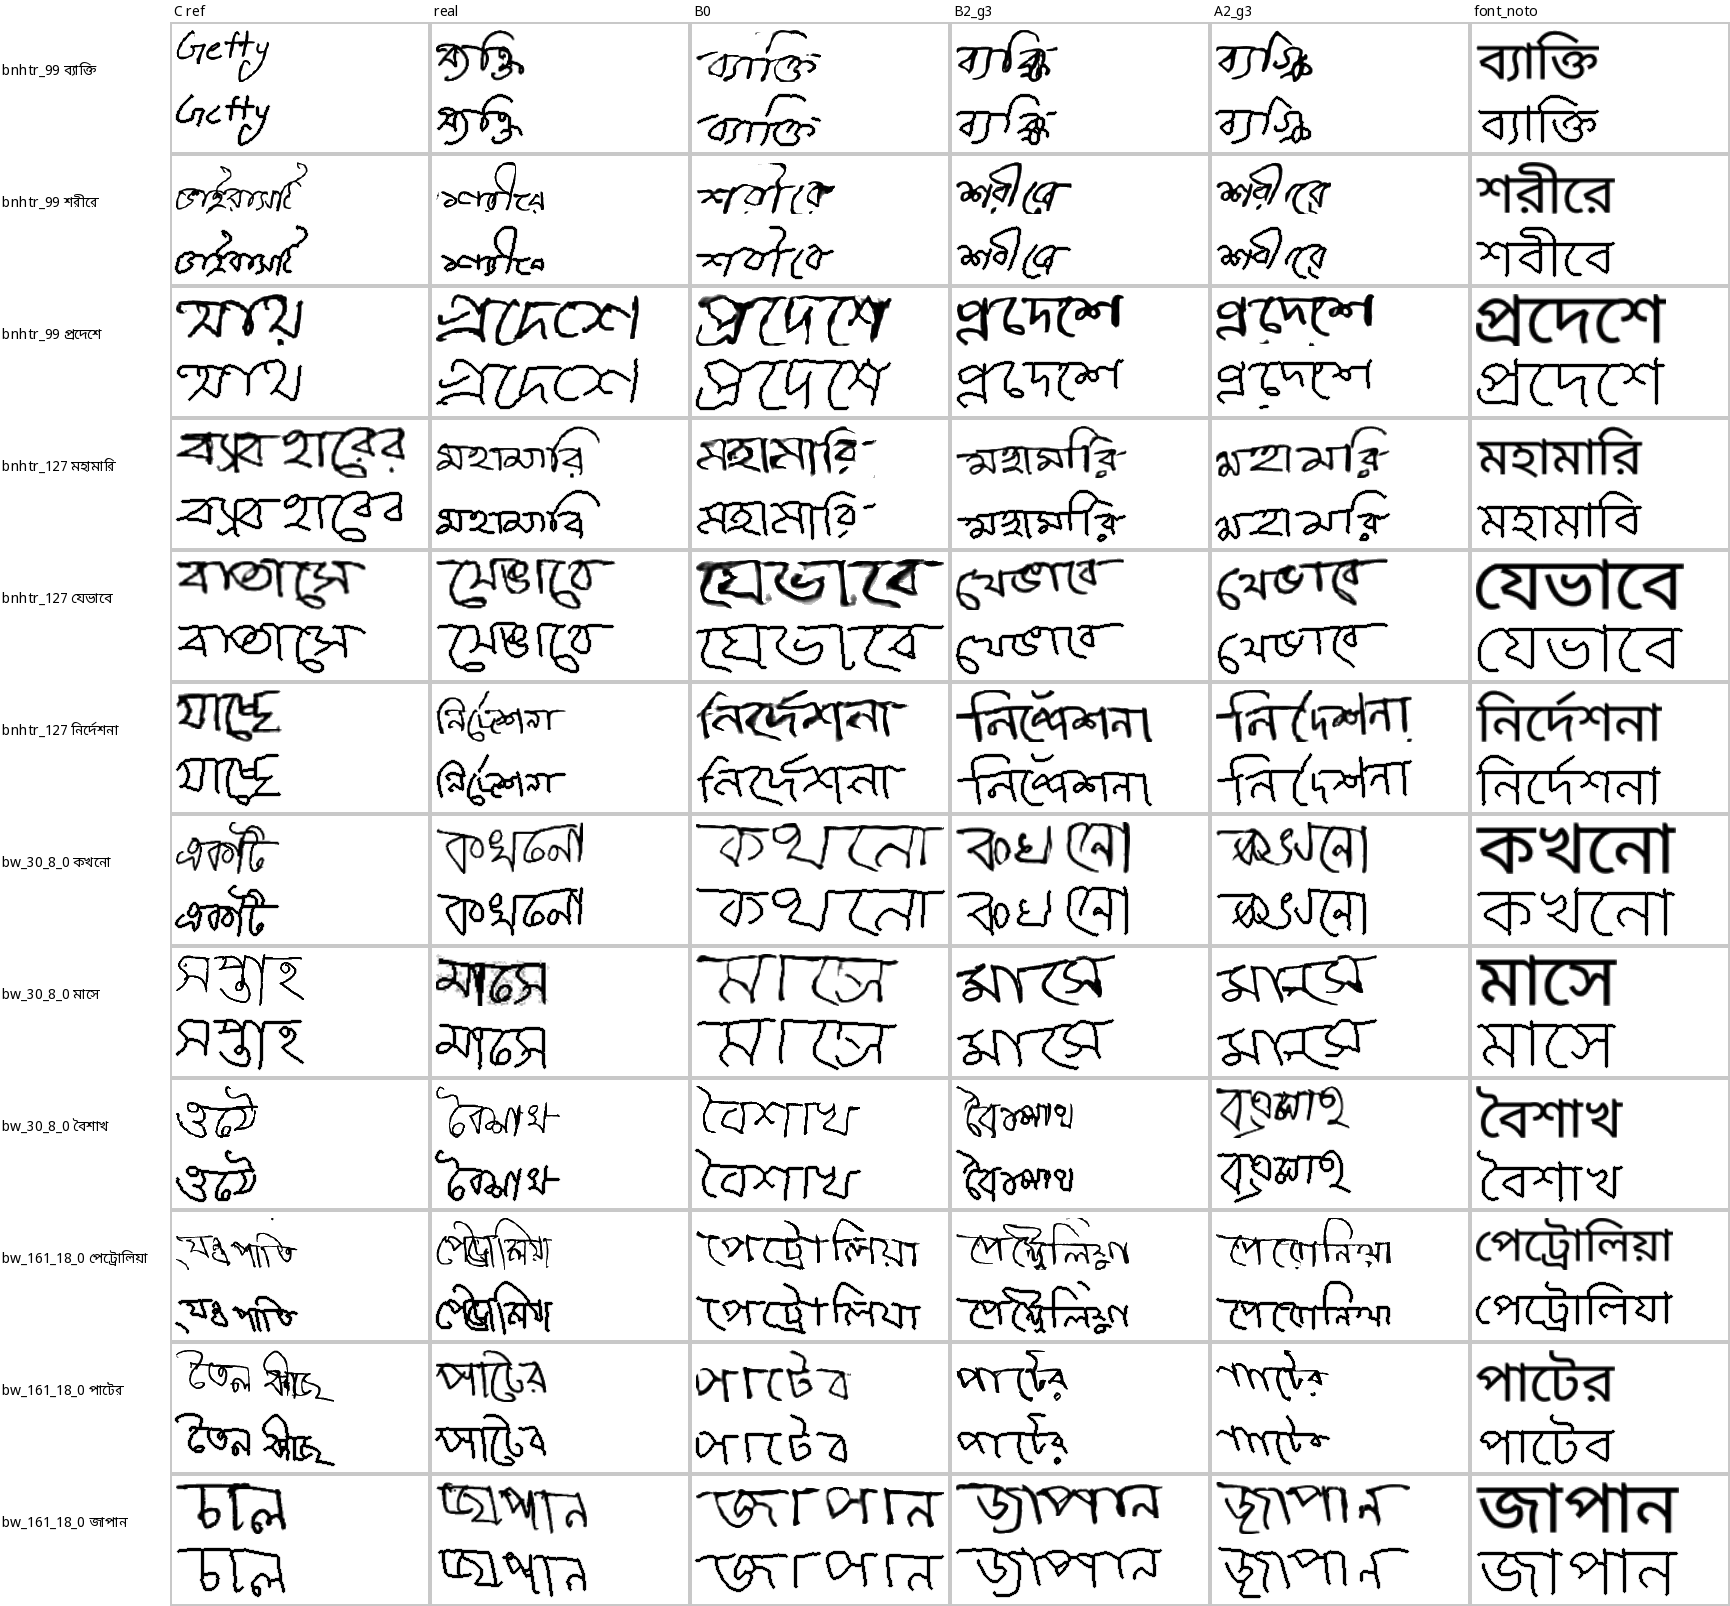
\includegraphics[width=0.78\linewidth]{q_style_prep.png}
\caption{Style-evaluator inputs after the shared preprocessing. Columns: a conditioning reference, the real target, B0,
\Bp{} g3, \Ap{} g3, NotoSans; two variants per row.}
\src{\fp{scribe_wordgen/runs/style_eval/sheet_prep.png}}
\end{figure}

\subsection{Pen calibration (post hoc, no retraining)}
Generation preserves the writer's pen \emph{rank}: Spearman over writers is about 0.9 in pixels. So a per-writer gain is
well posed. \fp{wordgen/pen/calibrate.py} re-renders strokes at page scale toward the refs' measured width.
Table~\ref{tab:pencal} compares the modes on \Bp{} t5c5. All modes bring the pen into $1.0\pm0.1$. The chosen shrink mode
(1.30$\to$1.05) misses the CER gate (upper CI of the CER change $\le+0.01$) by 0.0003. Only the per-writer mode passes both
gates, but its p90 over writers is 2.20.

\begin{table}[H]
\centering
\caption{Pen calibration modes on \Bp{} t5c5 (VAL; pen median over writers, CI of median).}
\label{tab:pencal}
\small
\begin{tabular}{@{}lcccc@{}}
\toprule
mode & pen ratio [CI] & p10--p90 & CER after$-$before & gates (pen / CER) \\
\midrule
before & 1.30 \ci{1.15}{1.45} & 1.06--1.85 & -- & -- \\
writer & 1.09 \ci{0.99}{1.29} & 0.87--2.20 & $+0.0027$ \ci{-0.0030}{+0.0083} & pass / pass \\
writer\_v2 & 1.06 \ci{0.92}{1.21} & 0.80--1.51 & $+0.0049$ \ci{-0.0007}{+0.0101} & pass / fail \\
global\_v2 & 1.07 \ci{1.00}{1.26} & 0.85--1.52 & $+0.0046$ \ci{-0.0011}{+0.0103} & pass / fail \\
word\_v2 & 1.05 \ci{0.92}{1.18} & 0.78--1.53 & $+0.0053$ \ci{-0.0011}{+0.0120} & pass / fail \\
\textbf{shrink\_v2 (adopted)} & 1.05 \ci{0.97}{1.18} & 0.83--1.37 & $+0.0051$ \ci{-0.0000}{+0.0103} & pass / fail by 0.0003 \\
\bottomrule
\end{tabular}
\src{\fp{scribe_wordgen/runs/pen_calib/report_Bp_t5c5_pencal_*.txt}}
\end{table}

\begin{figure}[H]
\centering
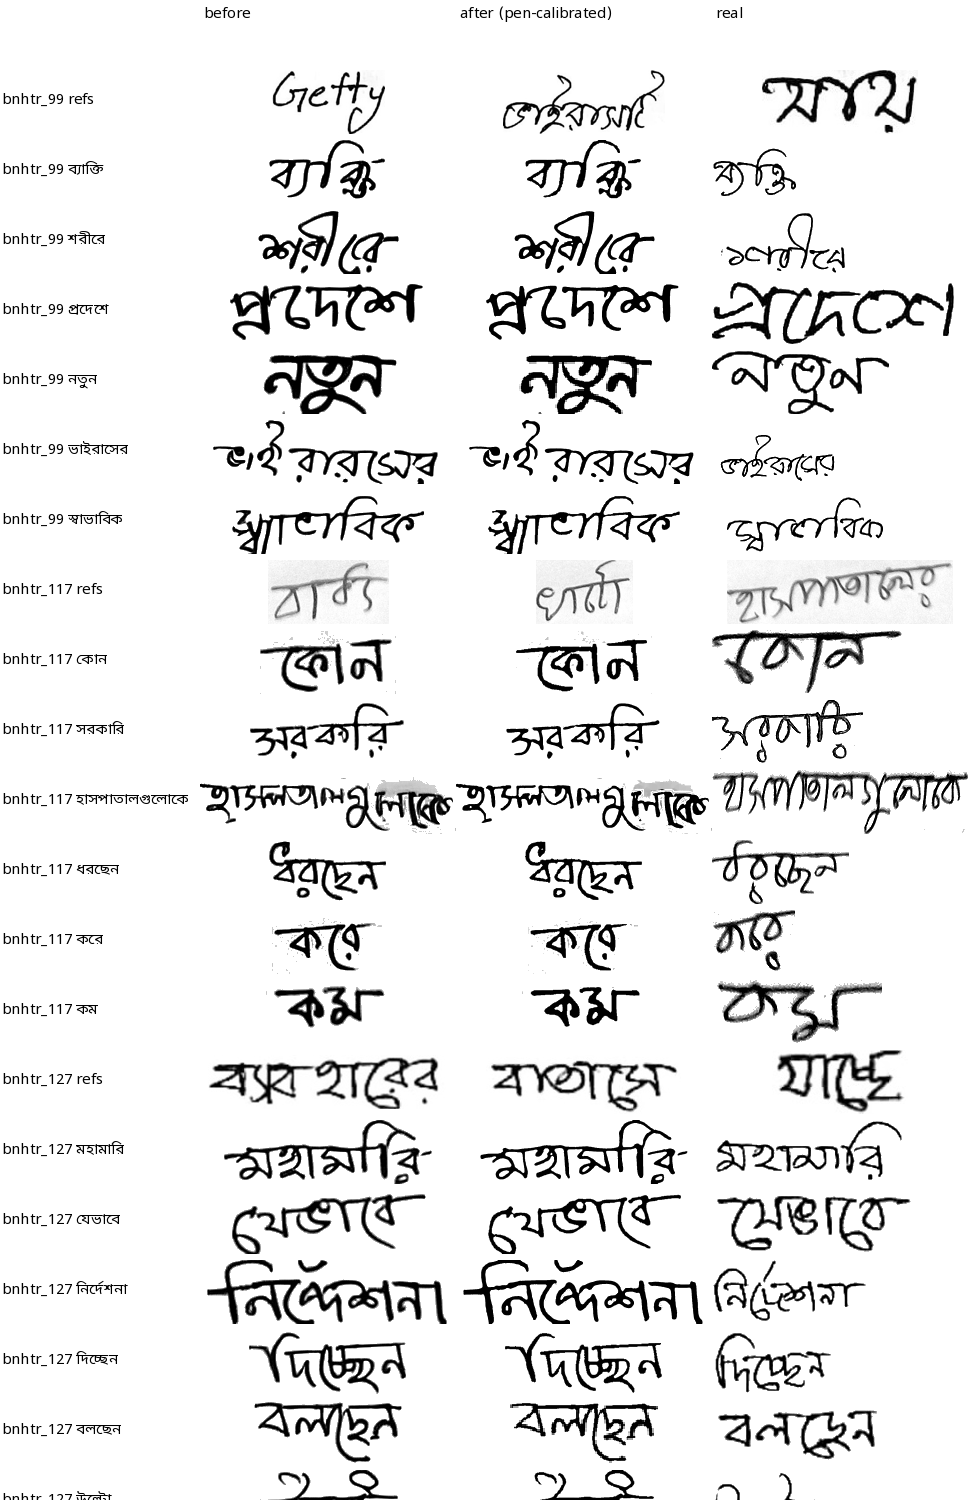
\includegraphics[width=0.55\linewidth]{q_pencal_top.png}
\caption{Pen calibration, shrink mode: \Bp{} t5c5 before (left), after (centre) and the writer's real crop (right).}
\src{\fp{scribe_wordgen/runs/pen_calib/sheet_Bp_t5c5_pencal_shrink_v2.png} (top part)}
\end{figure}

\subsection{bgnorm2: background normalisation v2}
The single-scalar whitening (90th-percentile paper $\to$ 255) left writer 117's references with a grey, graded box, which
the model reproduced as texture. \texttt{fit\_canvas\_white2} works on luminance only. It divides by a large-kernel
background estimate and soft-clips the paper to exactly 255, keeping ink darkness linear. On TRAIN crops it changes ink mass
by a median ratio of 0.998. It needs no retraining; the references must be passed through it (Table~\ref{tab:bg2}).

\begin{table}[H]
\centering
\caption{bgnorm2 on \Bp{} g3 (references only, no retraining).}
\label{tab:bg2}
\small
\begin{tabular}{@{}lcccc@{}}
\toprule
method & CER & bg-fail (non-punct) & faint blotch (mean) & blotch, writer 117 \\
\midrule
real & 0.133 \ci{0.100}{0.167} & 0.0\% & 0.4\% & 7.5\% \\
\Bp{} g3, v1 refs & 0.188 \ci{0.150}{0.226} & 0.8\% & 3.7\% & 30.0\% \\
\Bp{} g3, bgnorm2 refs & 0.183 \ci{0.142}{0.226} & 0.3\% & 1.8\% & 0.0\% \\
\bottomrule
\end{tabular}
\par\smallskip\footnotesize Paired CER (v2$-$v1 refs) $-0.0042$ \ci{-0.0170}{+0.0079} (11/20 writers). Writer 117 alone: CER
0.080$\to$0.116, blotch 30\%$\to$0\%.
\src{\fp{scribe_wordgen/runs/bgnorm2/bprime_noretrain.txt}, \fp{measure.txt}}
\end{table}

\begin{figure}[H]
\centering
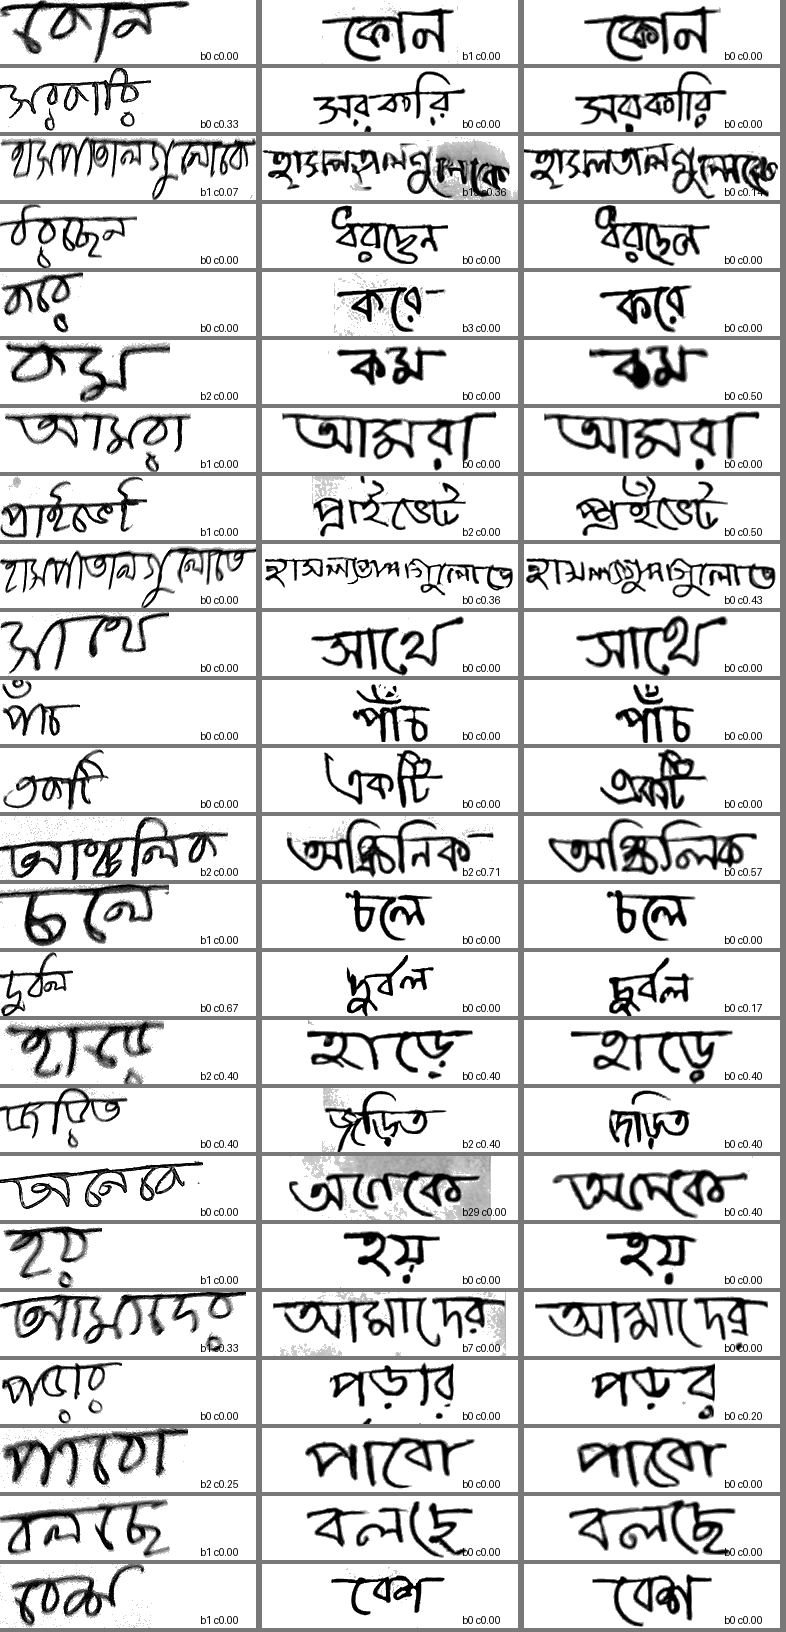
\includegraphics[width=0.38\linewidth]{q_bgnorm2_117.png}
\caption{Writer bnhtr\_117 (grey-paper scans). Columns: real crop, \Bp{} with v1 refs, \Bp{} with bgnorm2 refs. Each cell is
labelled with blotch (b) and CER (c).}
\src{\fp{scribe_wordgen/runs/bgnorm2/sheet_gen_bnhtr_117.png} (builder \fp{scratch/bgnorm2_gen_sheet.py})}
\end{figure}

\subsection{Arm P and Arm S}
\label{sec:armsPS}
Both arms warm-start from the \Bp{} checkpoint and train on 100,868 TRAIN rows encoded with bgnorm2. Training uses batch 32,
lr $10^{-4}$ (10$\times$ for new modules), 300 warm-up steps and a final lr fraction of 0.1. Dropouts are text, content and
style 0.1 and pen 0.05, and the CFG null drops all of them together. Sampling is rebalanced to punctuation 1.5\%, BW 38\% and
BN-HTR 60.5\%, against a natural mix of 2.0 / 15.4 / 82.6\%. Writers within a dataset are weighted by
clip(median pen / writer pen, 0.5, 2.0), which up-weights thin pens. The two arms differ as follows
(\fp{runs/P1a3/{P,S}/config.json}):
\begin{itemize}
\item \textbf{Pen knob} (both). The input is the refs' median $\log(w_\mathrm{sub}/c)$, z-scored with TRAIN statistics
  ($\mu=-1.835$, $\sigma=0.342$) and embedded sinusoidally. A zero-initialised MLP adds it to the timestep embedding, so the
  knob is a no-op at initialisation.
\item \textbf{Null-style fix} (both). In \Bp{}, dropped style fell back to the TRAIN writer-ID label embedding. P and S instead
  use a learned null style vector.
\item \textbf{Reference tokens} (S only). A Bengali writer encoder (ResNet-18, SupCon on TRAIN) turns each ref into 16
  spatial tokens. With slot embeddings, 5 refs give 80 tokens. They enter every transformer block through decoupled
  attention, $\mathrm{out}=\mathrm{attn}(q,\text{text+content})+\text{keep}\cdot W_\mathrm{ref}\,\mathrm{attn}(q,K_\mathrm{ref},V_\mathrm{ref})$.
  $W_\mathrm{ref}$ starts at zero, which keeps the no-op property. Appending the tokens to the shared context would not: 80
  extra keys change the softmax normalisation even with zero weights.
\end{itemize}
P trained for 16k steps (4,012\,s) and S for 24k steps (2,109\,s; final EMA loss 0.0581).

\paragraph{Two diverged S attempts and the gradient bug.} The first two S runs diverged. Run~1's rolling loss jumped from
$\approx$0.065 to above 0.14 within $\sim$800 steps. Run~2 drifted up from $\approx$0.064 to 0.108 by step 1,050 and was
stopped (Fig.~\ref{fig:curvesdiff}). The cause was a gradient bug. DiffusionPen's
\texttt{CheckpointFunction} re-runs each transformer block during backward. The side-channel attributes (\texttt{n\_ref} and
the keep mask) were reset after the forward pass, so the recomputation was a different function: full-context attention
without the reference branch. S therefore trained on wrong gradients. The fix keeps these attributes set; a test checks
that S's gradient matches a run without checkpointing (\fp{wordgen/models/diffusion3.py},
\fp{tests/test_p1a3.py}). The final S config also adds gradient clipping 1.0 and a 2$\times$ reference-token lr multiplier,
which the diverged configs lack.

\begin{figure}[H]
\centering
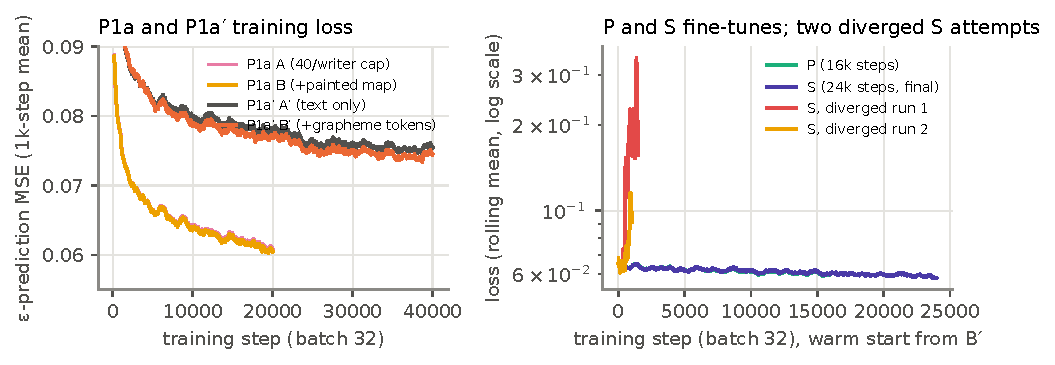
\includegraphics[width=\linewidth]{curves_diffusion.pdf}
\caption{Training curves. Left: P1a (capped data) and P1a$'$ (full data). The full-data loss level is higher because the
data are harder and more varied; the curves are not comparable across data sets. Right: P and S fine-tunes from \Bp, and the
two diverged S runs (log scale).}
\label{fig:curvesdiff}
\src{\fp{scribe_wordgen/runs/P1a{,2}/{A,B}/metrics.csv}, \fp{runs/P1a3/{P,S,S_diverged_v1,S_diverged_v2}/metrics.csv}}
\end{figure}

\begin{table}[H]
\centering
\caption{P and S on VAL (locator CER, 2 seeds; background and pen). \_cal = shrink-mode pen calibration.}
\label{tab:ps}
\small
\begin{tabular}{@{}lccccccc@{}}
\toprule
method & CER & 1--2 graph & $>$2 graph & OOV & bg-fail non-punct & blotch 117 & pen raw [CI] \\
\midrule
real & 0.133 \ci{0.100}{0.167} & 0.130 & 0.135 & 0.150 & 0.0\% & 8\% & 1.00 \\
B0 & 0.130 \ci{0.103}{0.156} & 0.115 & 0.143 & 0.235 & 0.0\% & 0\% & 1.15 \ci{0.98}{1.20} \\
\Bp{}v2 t5c5 & 0.151 \ci{0.117}{0.186} & 0.146 & 0.157 & 0.246 & 0.6\% & 1\% & 1.29 \ci{1.18}{1.46} \\
P t3c3 & 0.157 \ci{0.118}{0.198} & 0.185 & 0.128 & 0.226 & 3.0\% & 0\% & 1.13 \ci{1.02}{1.28} \\
\textbf{P t5c5} & 0.132 \ci{0.097}{0.171} & 0.163 & 0.104 & 0.194 & 2.7\% & 0\% & 1.15 \ci{1.01}{1.30} \\
S t3c3 & 0.153 \ci{0.115}{0.189} & 0.192 & 0.118 & 0.216 & 3.6\% & 0\% & 1.12 \ci{1.05}{1.21} \\
\textbf{S t5c5} & 0.137 \ci{0.101}{0.174} & 0.173 & 0.104 & 0.202 & 3.0\% & 0\% & 1.13 \ci{1.07}{1.21} \\
P t5c5\_cal & 0.133 & 0.165 & 0.105 & 0.195 & 2.6\% & 0\% & 1.06 \ci{0.97}{1.15} \\
S t5c5\_cal & 0.138 & 0.175 & 0.103 & 0.209 & 3.1\% & 0\% & 1.06 \ci{0.98}{1.12} \\
\bottomrule
\end{tabular}
\par\smallskip\footnotesize Paired CER: P$-$B0 $+0.002$ \ci{-0.028}{+0.037} (10/20); S$-$B0 $+0.007$ \ci{-0.023}{+0.040}
(10/20); S$-$P $+0.006$ \ci{-0.004}{+0.015}; P$-$\Bp{}v2 $-0.019$ \ci{-0.034}{-0.004} (16/20). OOV S$-$B0 $-0.033$
\ci{-0.088}{+0.016}. \textbf{The 1--2-grapheme column and bg-fail for P/S carry the \texttt{img\_to\_ink} short-word
artefact} (\S\ref{sec:smudge}).
\src{\fp{scribe_wordgen/runs/P1a3/eval/report_tables.txt}}
\end{table}

\begin{table}[H]
\centering
\caption{Style for P and S: M2 (E\_eval) and M2s (E\_shape) MRR, VAL, hierarchical bootstrap.}
\label{tab:psstyle}
\small
\begin{tabular}{@{}lcccc@{}}
\toprule
method & M2 MRR (all) & M2 BN-HTR / BW & M2s MRR (all) & M2s BN-HTR / BW \\
\midrule
real & 0.821 \ci{0.775}{0.859} & 0.916 / 0.789 & 0.768 \ci{0.724}{0.812} & 0.927 / 0.715 \\
B0 & 0.596 \ci{0.488}{0.711} & 0.883 / 0.500 & 0.533 \ci{0.453}{0.617} & 0.841 / 0.430 \\
\Bp{}v2 t5c5 & 0.418 \ci{0.355}{0.483} & 0.566 / 0.369 & 0.399 \ci{0.351}{0.449} & 0.609 / 0.330 \\
P t5c5 & 0.443 \ci{0.379}{0.505} & 0.556 / 0.405 & 0.416 \ci{0.367}{0.469} & 0.596 / 0.357 \\
\textbf{S t5c5} & \textbf{0.579} \ci{0.521}{0.635} & 0.745 / 0.523 & \textbf{0.517} \ci{0.469}{0.564} & 0.726 / 0.448 \\
S t5c5\_cal & 0.562 \ci{0.511}{0.615} & 0.716 / 0.511 & 0.518 \ci{0.471}{0.566} & 0.729 / 0.447 \\
\bottomrule
\end{tabular}
\par\smallskip\footnotesize Paired M2: S$-$B0 $-0.017$ \ci{-0.116}{+0.088} ($p=0.72$, 9/20); S$-$P $+0.136$
\ci{+0.085}{+0.187} (17/20); P$-$B0 $-0.153$ \ci{-0.261}{-0.048}. M2s: S$-$P $+0.101$ \ci{+0.057}{+0.140}; S$-$B0 $-0.015$
\ci{-0.091}{+0.061}. Chance: all 0.28; BN-HTR 0.457; BW 0.221.
\src{\fp{scribe_wordgen/runs/P1a3/eval/report_tables.txt}, \fp{runs/P1a3/eval/metrics.json}}
\end{table}

All P/S variants pass the planned gates from the P1a$'$ review: CER $\le$ B0+0.05 = 0.180, calibrated pen $\le$1.15, and
writer-117 blotch $<$10\%.

\begin{figure}[H]
\centering
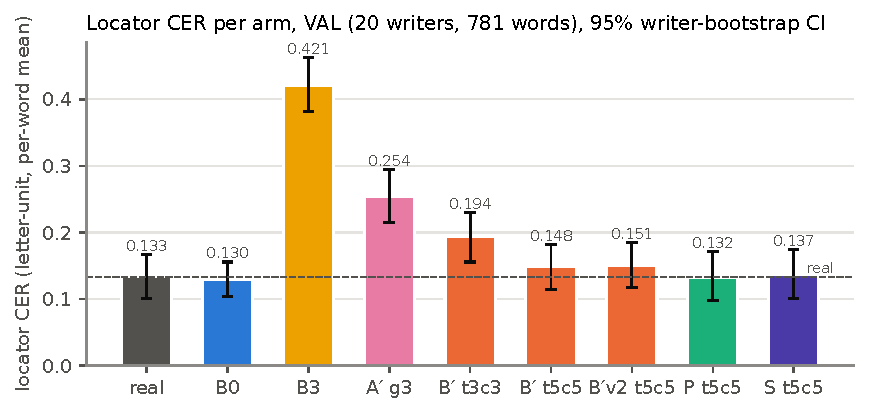
\includegraphics[width=0.95\linewidth]{cer_locator_arms.pdf}
\caption{Locator CER per arm (letter units; capped per-word mean). From \Bp{} t5c5 on, every diffusion arm ties B0 on this
metric.}
\src{\fp{runs/eval_v3/metrics.json}, \fp{runs/P1a3/eval/metrics.json}}
\end{figure}

\begin{figure}[H]
\centering
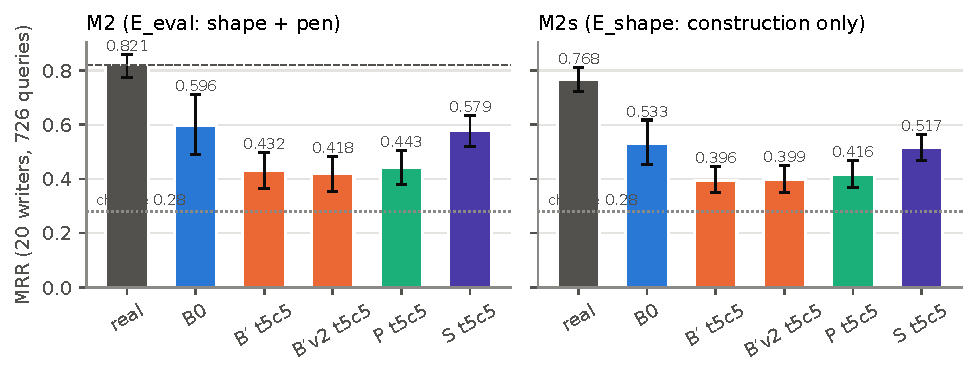
\includegraphics[width=0.95\linewidth]{style_mrr_arms.pdf}
\caption{Style MRR per arm, with the chance line (dotted) and the real-crop level (dashed, left). The reference tokens of S
lift style from the 0.42--0.44 plateau of \Bp/P to B0's level.}
\src{\fp{runs/P1a3/eval/metrics.json}}
\end{figure}

\begin{figure}[H]
\centering
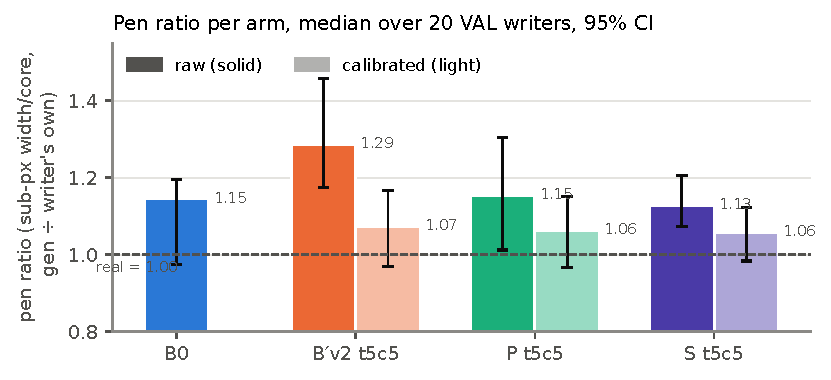
\includegraphics[width=0.85\linewidth]{pen_ratio.pdf}
\caption{Pen ratio, raw and calibrated (median over 20 writers, 95\% CI of the median).}
\src{\fp{runs/P1a3/eval/metrics.json}}
\end{figure}

\paragraph{Pen-knob sweep.} The knob was multiplied by 0.6--1.6 (g5, seed 0, 8 words $\times$ 20 writers;
Fig.~\ref{fig:knob}). In P the within-writer slope $d\log(\text{generated})/d\log(\text{knob})$ is 0.11 \ci{0.08}{0.14}: the knob
works but is weak. In S it is 0.03 \ci{0.00}{0.05}, \textbf{nearly inert}. The reference tokens apparently carry the pen and
override the scalar. Across writers without a sweep, generated width tracks the knob with slope 0.15 in both arms (Spearman
0.31 P, 0.15 S).

\begin{figure}[H]
\centering
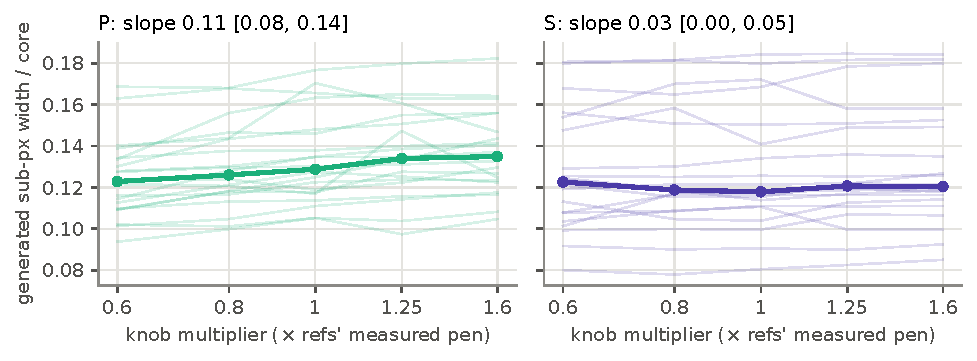
\includegraphics[width=0.92\linewidth]{pen_knob_sweep.pdf}
\caption{Pen-knob sweep. Thin lines: per-writer medians; bold: median over writers. Titles give the within-writer slope with its
95\% CI over writers.}
\label{fig:knob}
\src{\fp{runs/P1a3/eval/sweep.csv}, \fp{runs/P1a3/eval/metrics.json} (\texttt{knob\_sweep})}
\end{figure}

\begin{figure}[H]
\centering
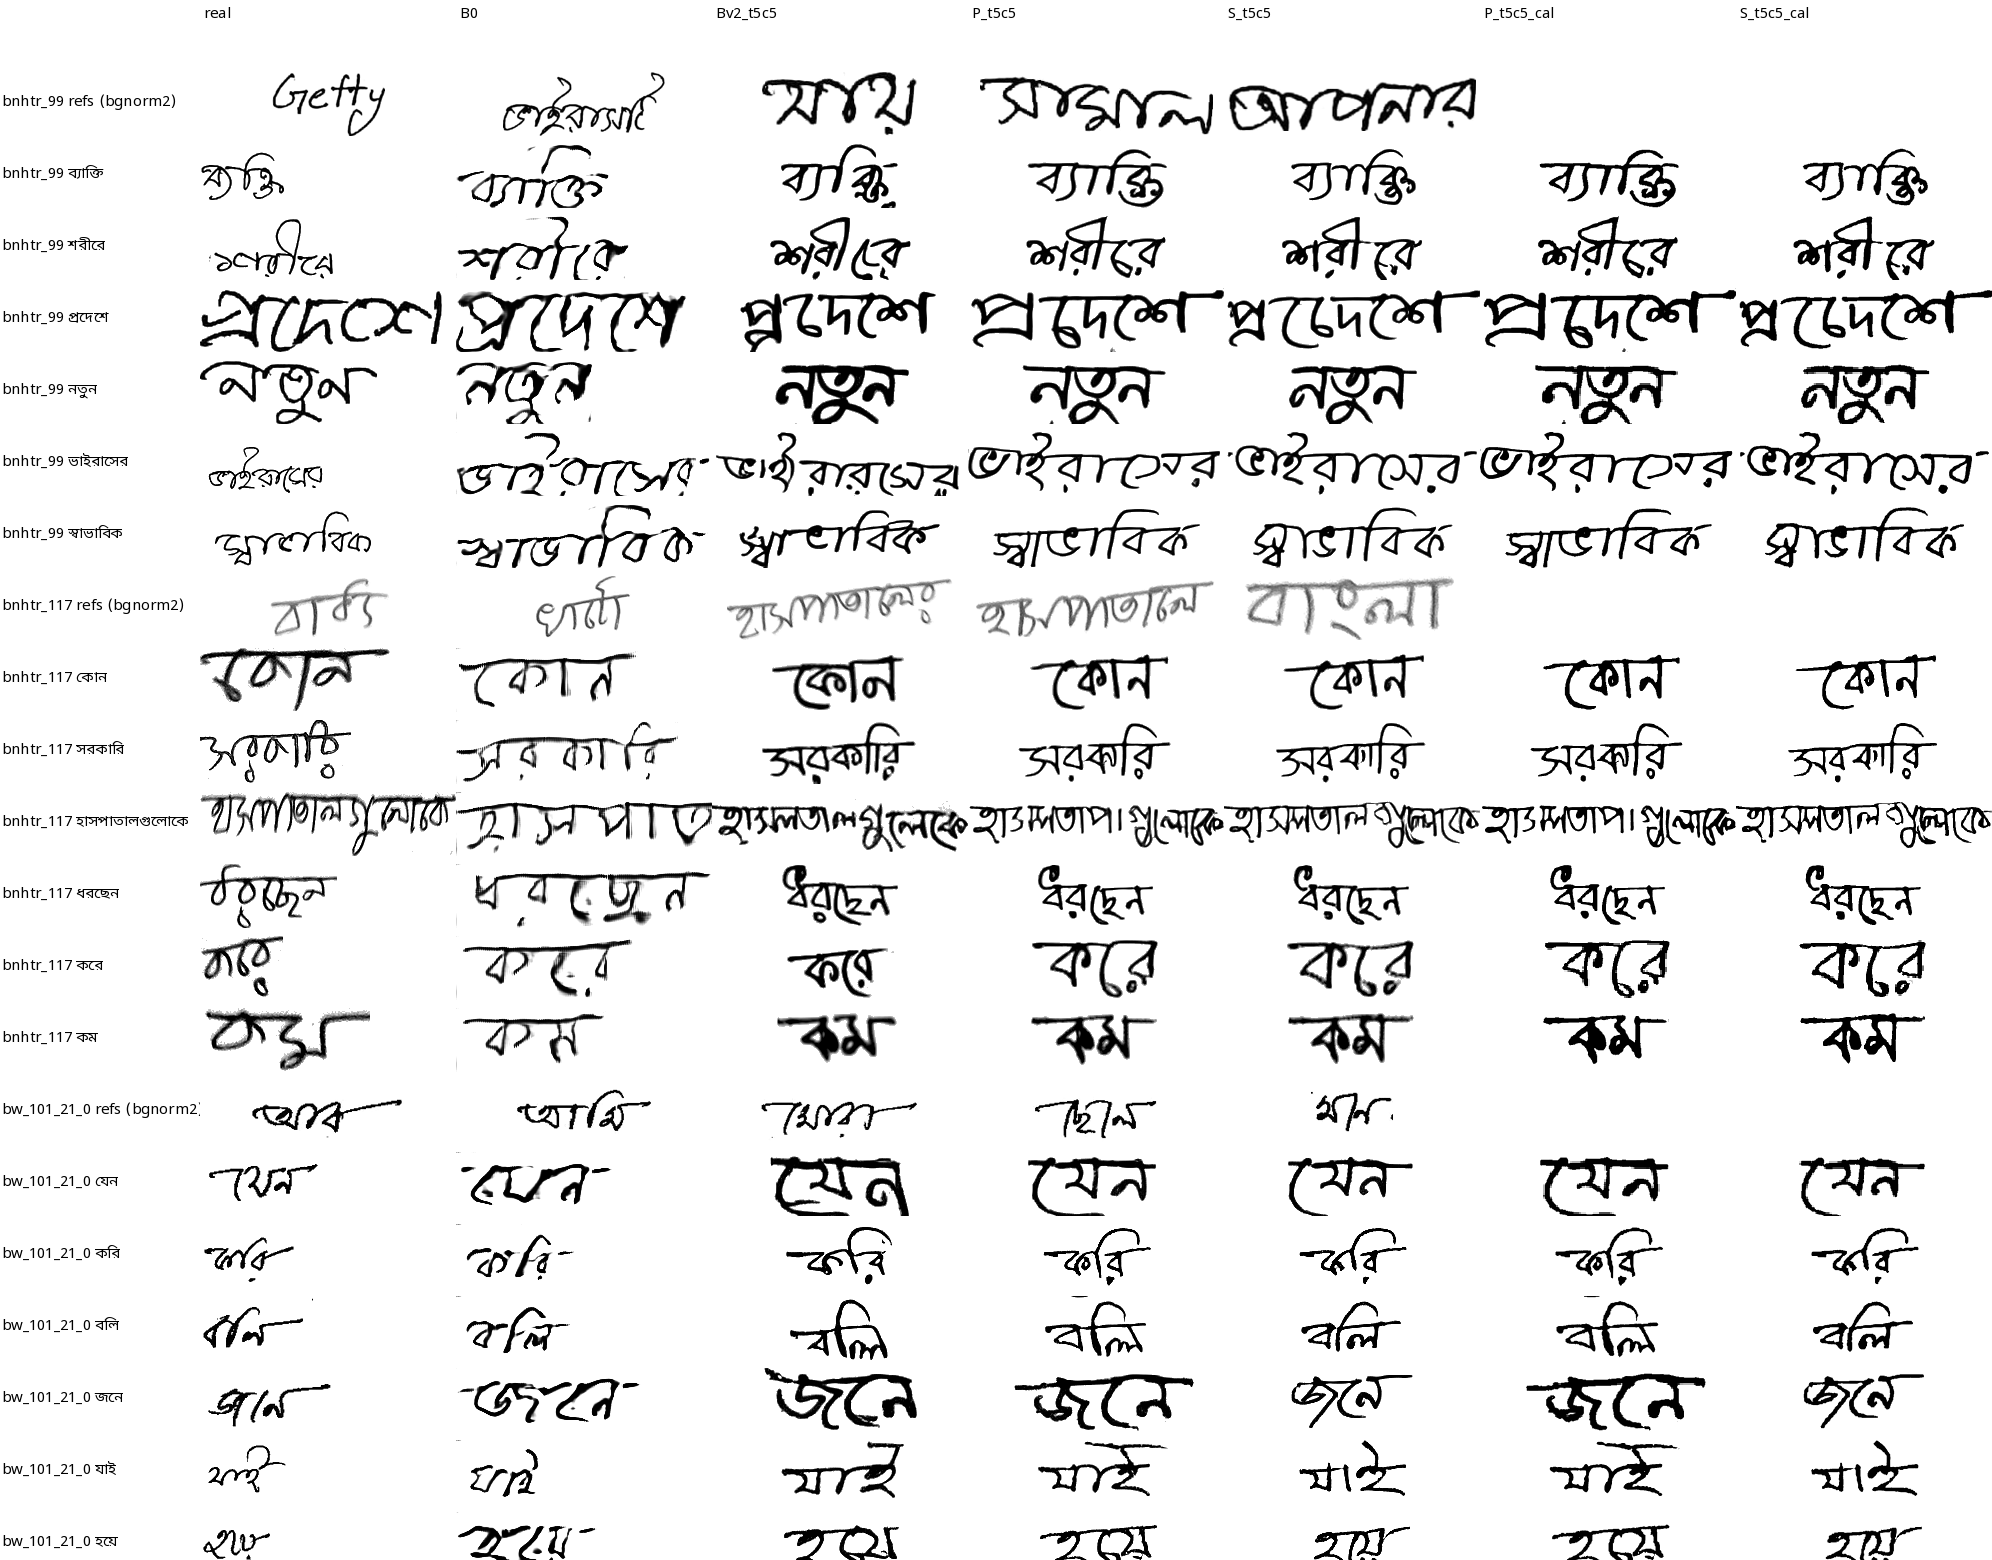
\includegraphics[width=0.9\linewidth]{q_p1a3_sheet_val_top.png}
\caption{VAL words (top of the P1a3 sheet; seed 0). Columns: real, B0, \Bp{}v2 t5c5, P t5c5, S t5c5, P calibrated, S
calibrated. ``refs (bgnorm2)'' rows show the writer's conditioning crops.}
\src{\fp{scribe_wordgen/runs/P1a3/eval/sheet_val.png}}
\end{figure}

\subsection{Page sheets and the smudge fix}
\label{sec:smudge}
Full pages were rendered with the learned layout (\fp{scribe_layout_v2/runs/default_unfitw_dc/model.pt}) for B0, \Bp, P and S.
The writers were image\_2 and three VAL writers (\fp{runs/page_sheets/}). Two problems are visible
(Fig.~\ref{fig:pages}). Generated text on BanglaWriting pages renders smaller than the real page, and P draws dash words
(``--'') as thick bars.

\paragraph{The ``smudges'' were not the model.} Isolated glyphs such as \bnt{০}, \bnt{ও} and \bnt{২} came out as dark
smudges. The cause is in \texttt{img\_to\_ink}. Its 5th-percentile ink floor assumes ink covers $\ge$5\% of the canvas. A
lone glyph covers 2--3\%, so the floor lands on paper texture and a ripple of about 12 grey levels is stretched to black.
The fix \texttt{img\_to\_ink(..., min\_span=100)} keeps the floor at least 100 grey levels below paper. It brings the
lone-glyph ink fraction from 39--56\% down to 2--3\% and leaves normal words unchanged. The fix is opt-in. \textbf{The eval
caches still use the legacy conversion}, so short-word CER and blotch for the diffusion arms P, \Bp{} and S carry the
artefact until all arms are rescored together. The old inks are kept in \fp{runs/page_sheets/cache_v1_smudged/}.

\begin{figure}[H]
\centering
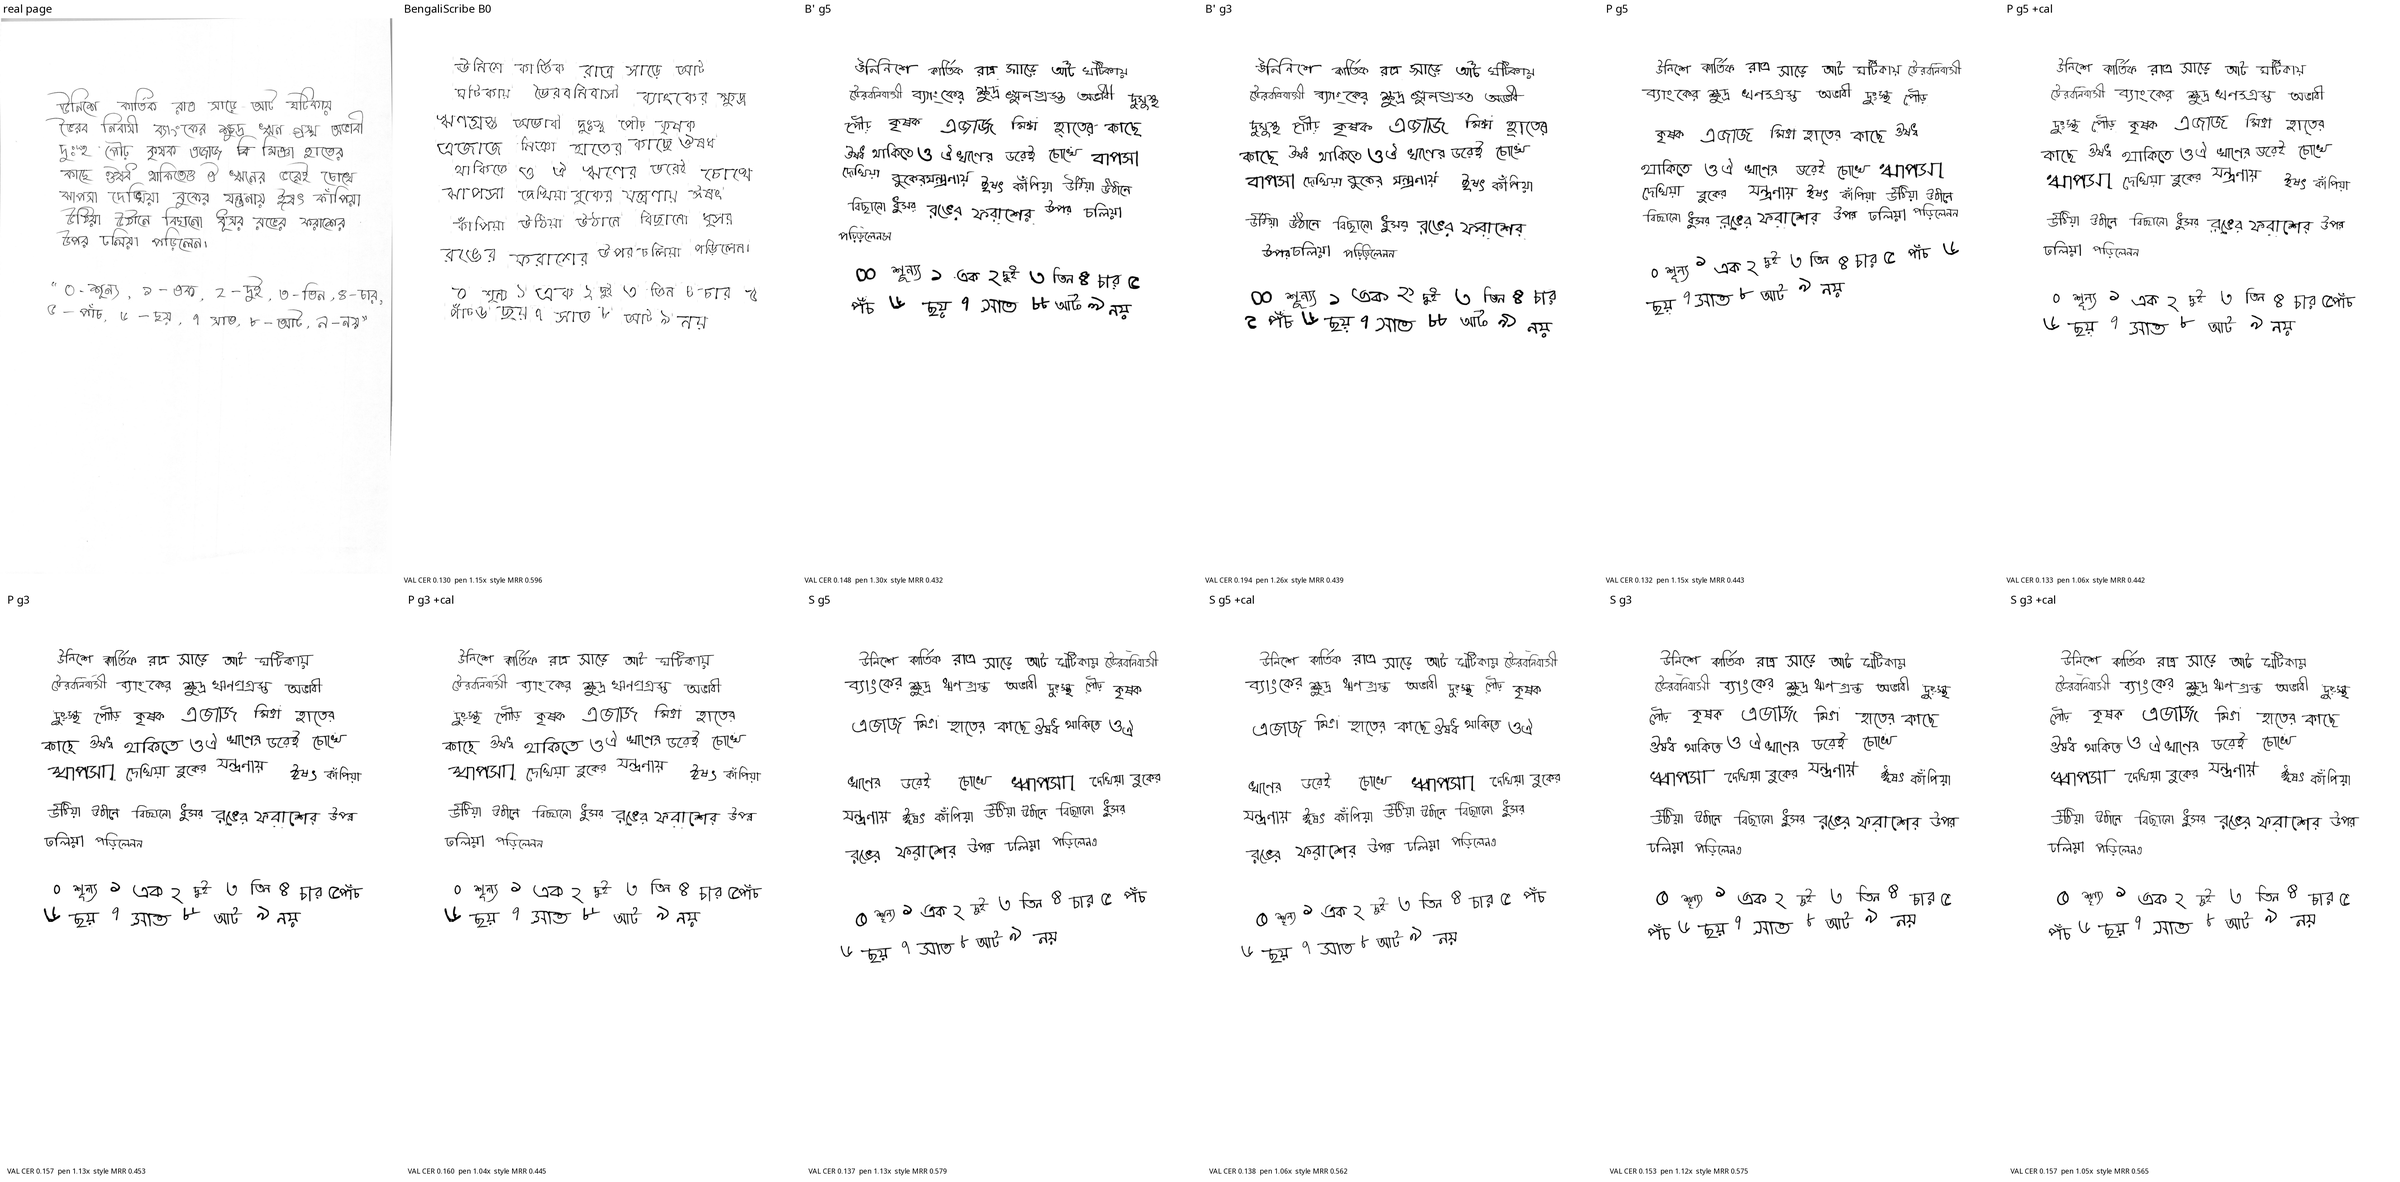
\includegraphics[width=\linewidth]{q_pagesheet_image_2.png}
\caption{Page sheet for image\_2, split into two rows of six panels. Row 1: real page, B0, \Bp{} g5, \Bp{} g3, P g5, P g5
calibrated. Row 2: P g3, P g3 calibrated, S g5, S g5 calibrated, S g3, S g3 calibrated.}
\label{fig:pages}
\src{\fp{scribe_wordgen/runs/page_sheets/sheets/image_2_sheet_l0.png}}
\end{figure}

\begin{figure}[H]
\centering
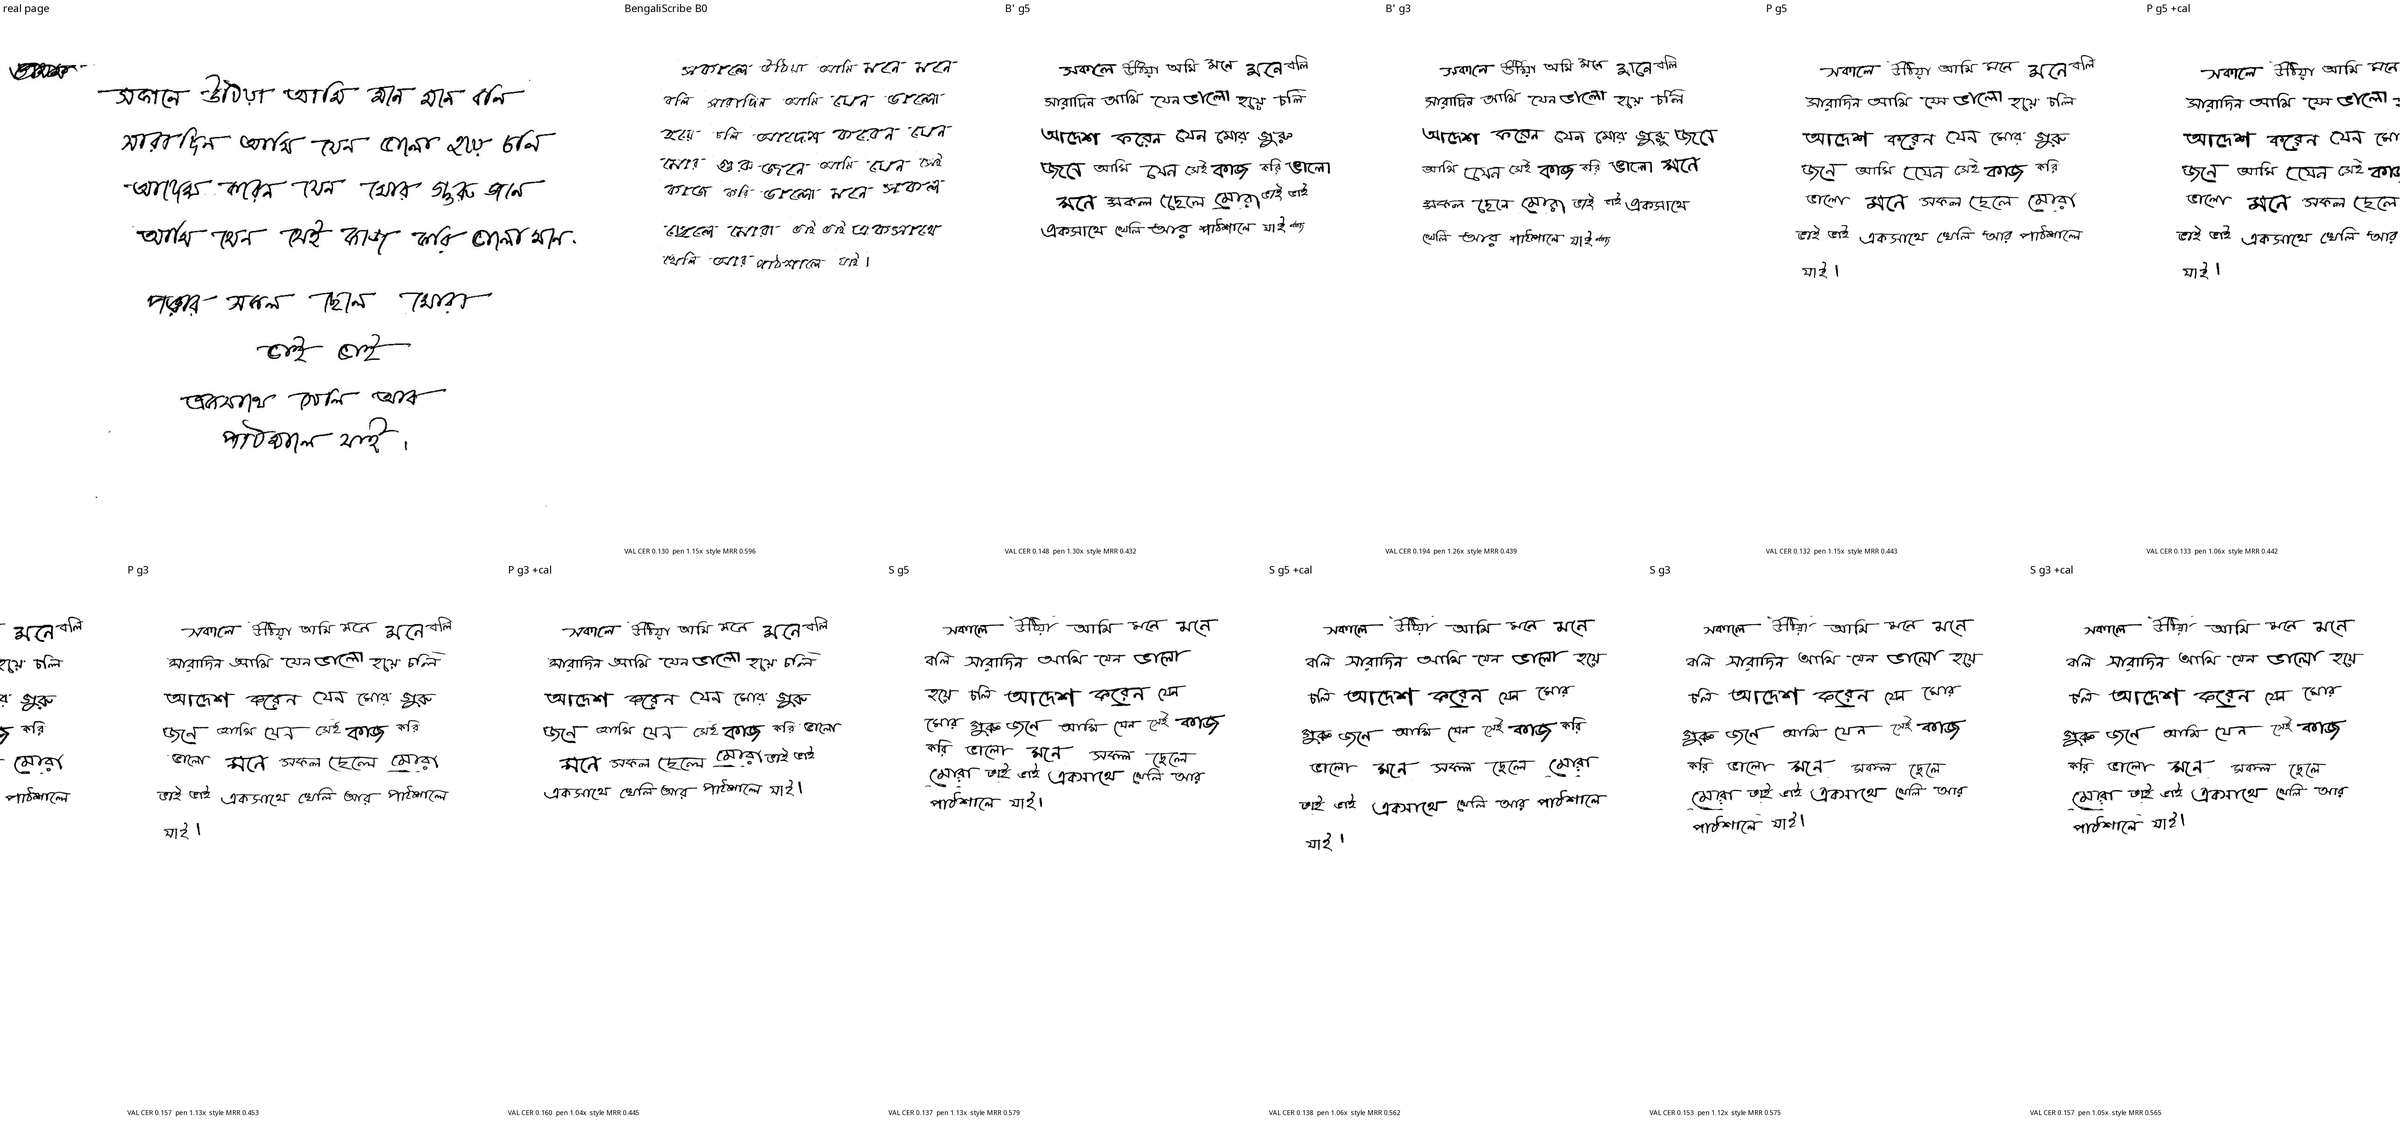
\includegraphics[width=\linewidth]{q_pagesheet_bw_101_21_0.png}
\caption{Page sheet for BanglaWriting VAL writer bw\_101\_21\_0 (same panel order). The generated text is smaller than the
real writer's.}
\src{\fp{scribe_wordgen/runs/page_sheets/sheets/bw_101_21_0_sheet_l0.png}}
\end{figure}

\begin{figure}[H]
\centering
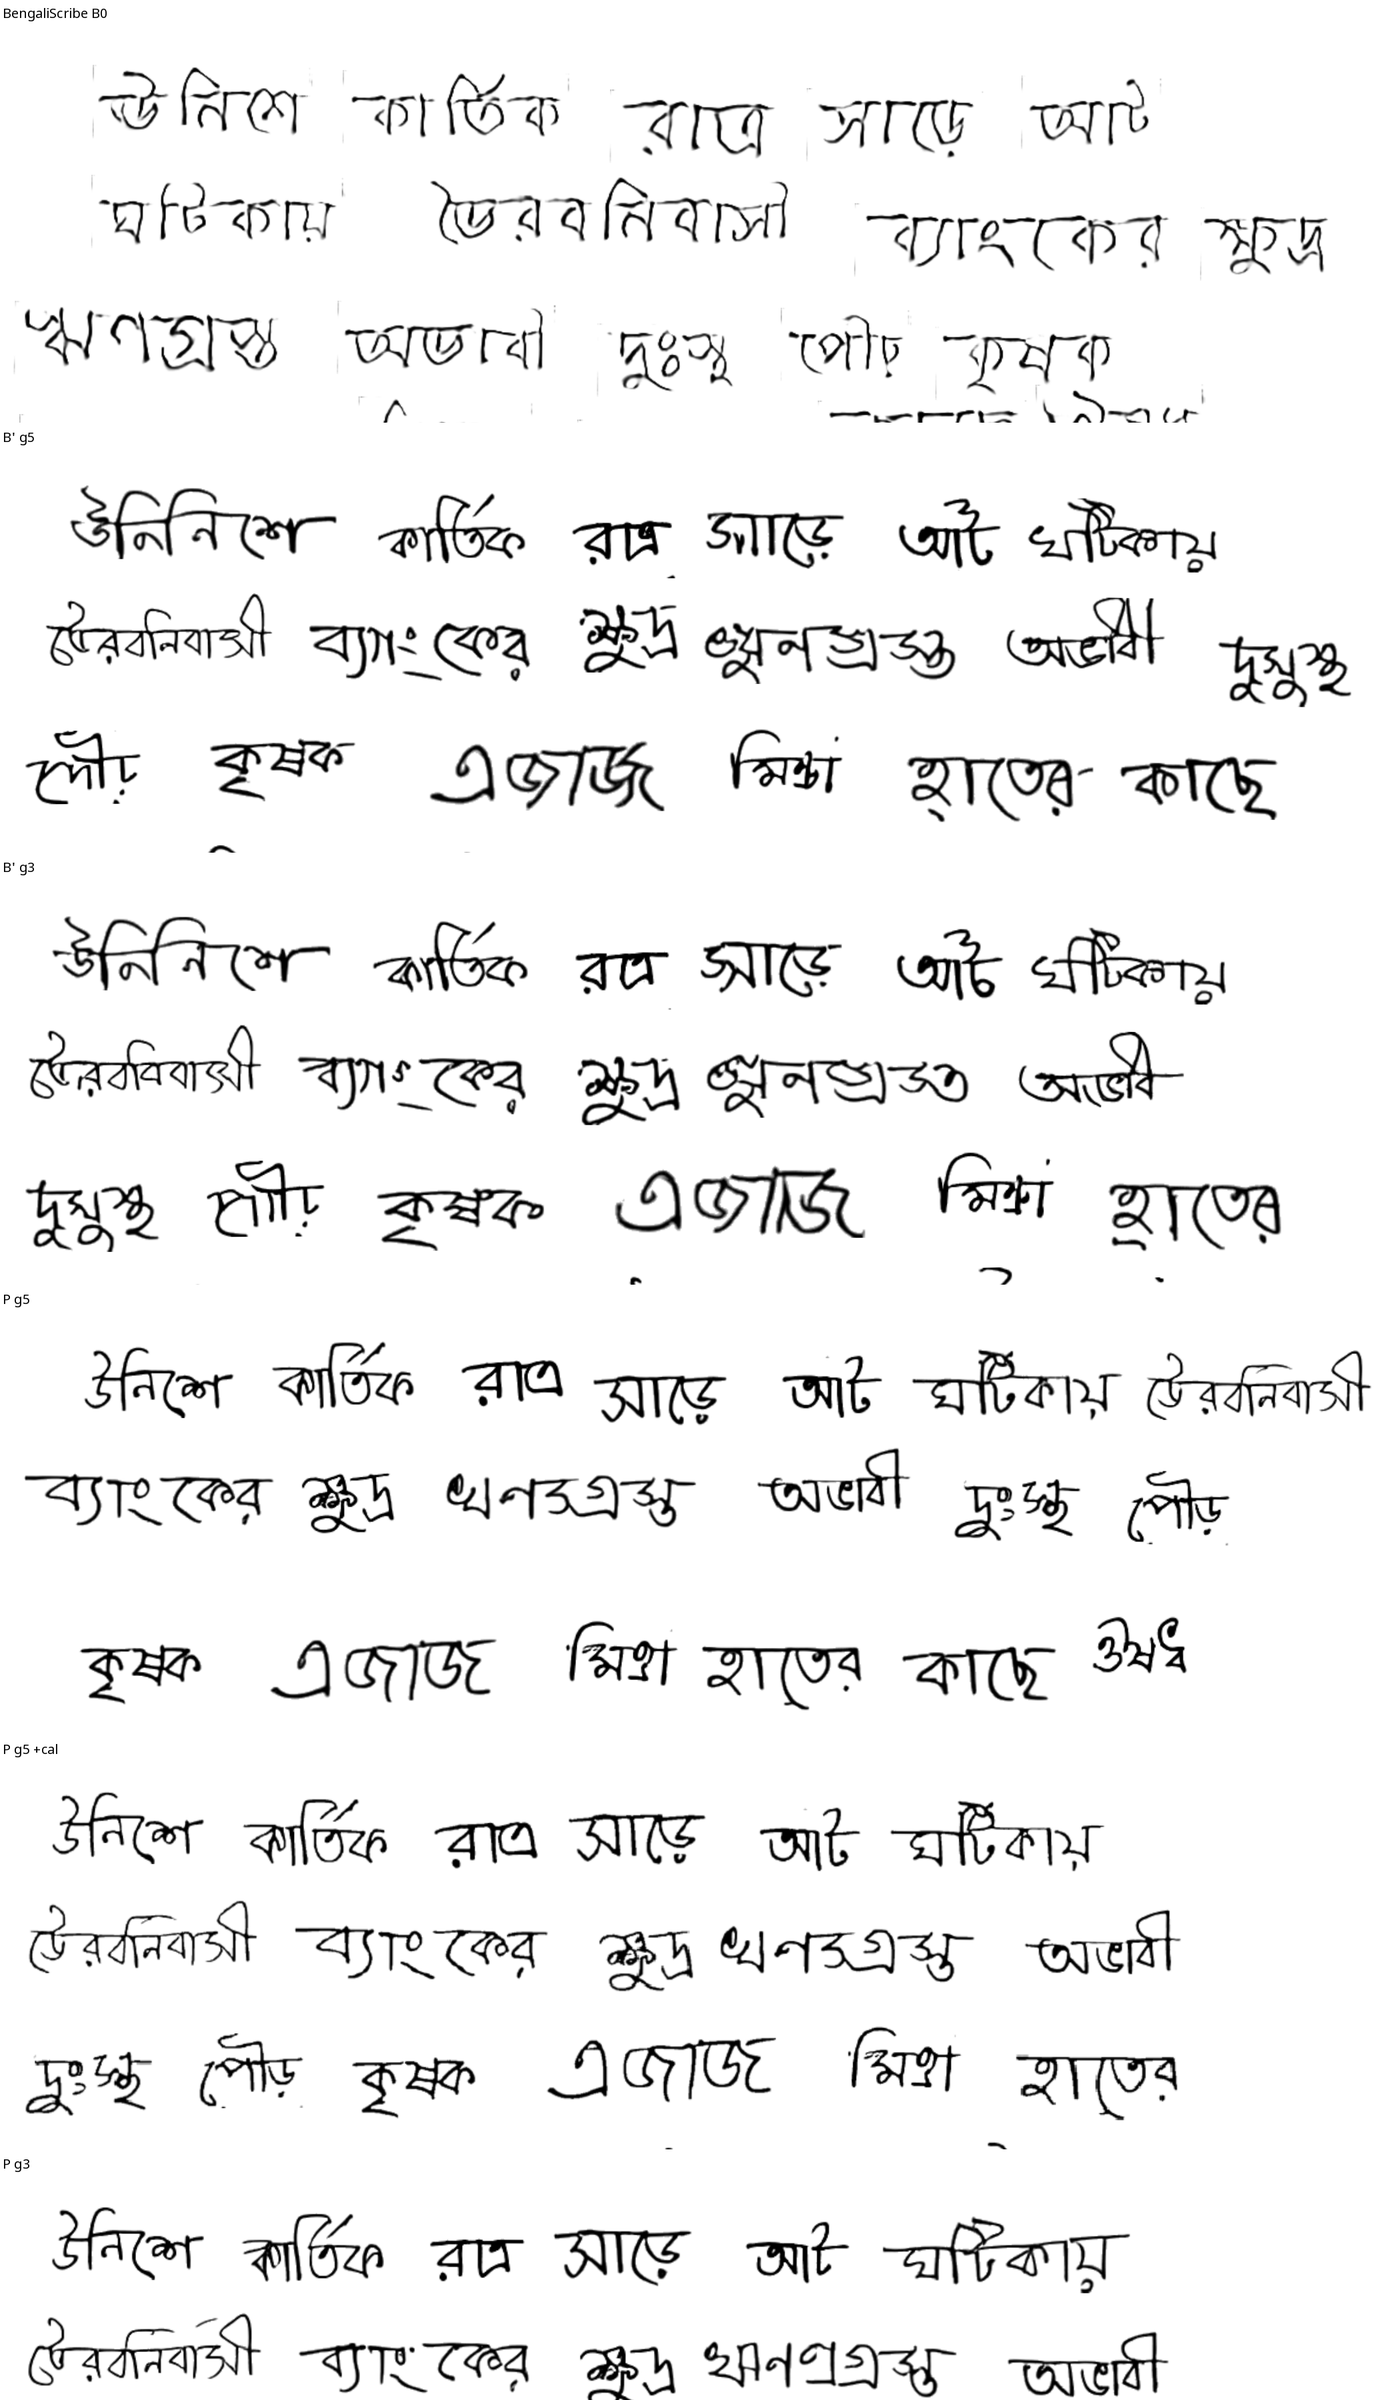
\includegraphics[width=0.62\linewidth]{q_pagezoom_image_2_top.png}
\caption{Zoom on the first lines of the image\_2 page: B0, then \Bp{} g5, \Bp{} g3, P g5 and P g5 calibrated.}
\src{\fp{scribe_wordgen/runs/page_sheets/sheets/image_2_zoom_l0.png} (top part)}
\end{figure}

%=============================================================================
\section{GlyphScribe fonts and the R\_eval recogniser}
\label{sec:fonts}

\subsection{Fonts}
The first font search scored 11 Google OFL Bengali fonts against image\_2 (12 hand-verified words) by skeleton chamfer.
Atma, Hind Siliguri and Noto Serif Bengali came out closest, with overlapping CIs; NotoSans ranked 11th of 12
(\fp{runs/font_search/REPORT.md}). Then 37 handwriting fonts, 1 printed font and 4 paper backgrounds were copied from the
public GlyphScribe repository. Its licence covers the code only and the font licences are unknown, so these fonts are for
internal research only. All 38 are Unicode Bengali with correct GSUB shaping. On shape, Atma variants rank first (chamfer
0.162--0.164) and NotoSans ranks 28th of 39. The top $\sim$10 fonts overlap within their CIs (Fig.~\ref{fig:fonts}). Thin
fonts match the pen far better: the writer's width/core is 0.075, against 0.094 for Junudullah Zami and Tagore, 0.068 for
Qayyum Thin and 0.11--0.23 for the Google fonts. No font draws the writer's broken matra.

\begin{figure}[H]
\centering
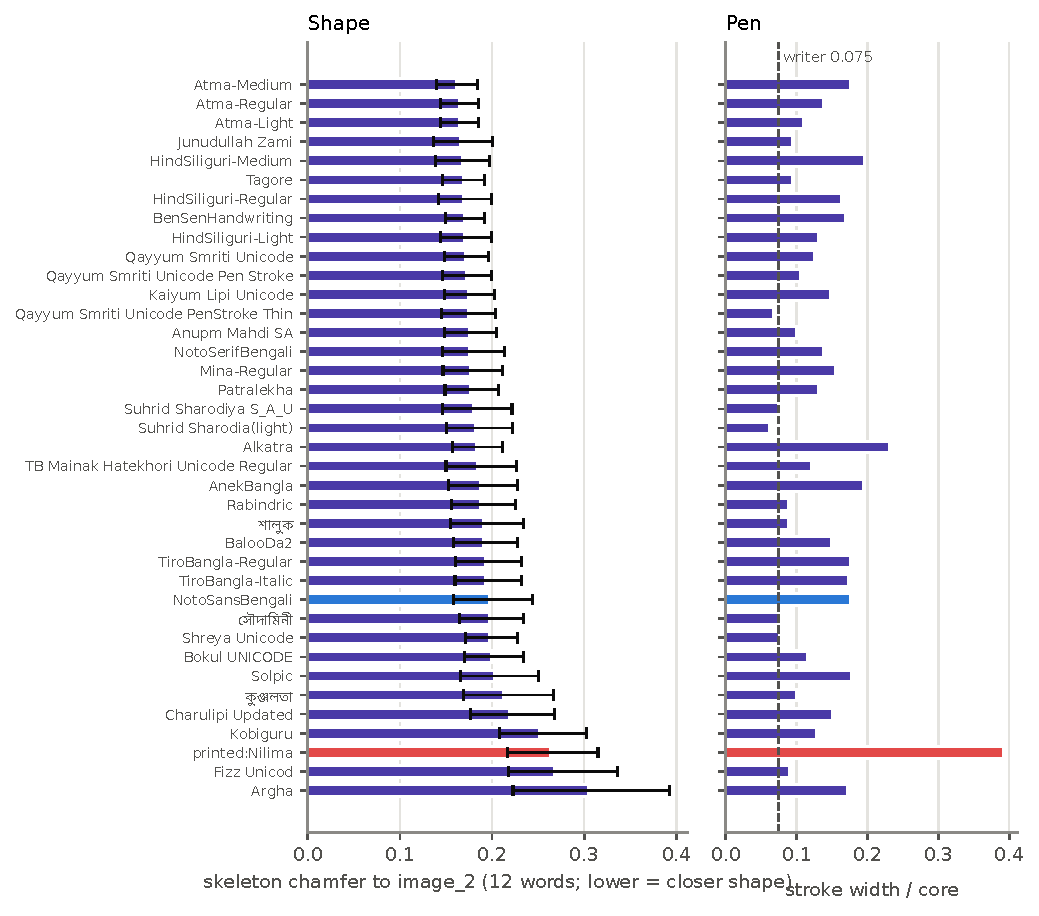
\includegraphics[width=0.92\linewidth]{fonts_glyphscribe.pdf}
\caption{All scored fonts against image\_2: skeleton chamfer with 95\% CI over 12 words (left), stroke width/core (right).
Blue: NotoSans (BS's font). Red: the printed font.}
\label{fig:fonts}
\src{\fp{scribe_wordgen/runs/font_search/glyphscribe/scores.csv}}
\end{figure}

\begin{figure}[H]
\centering
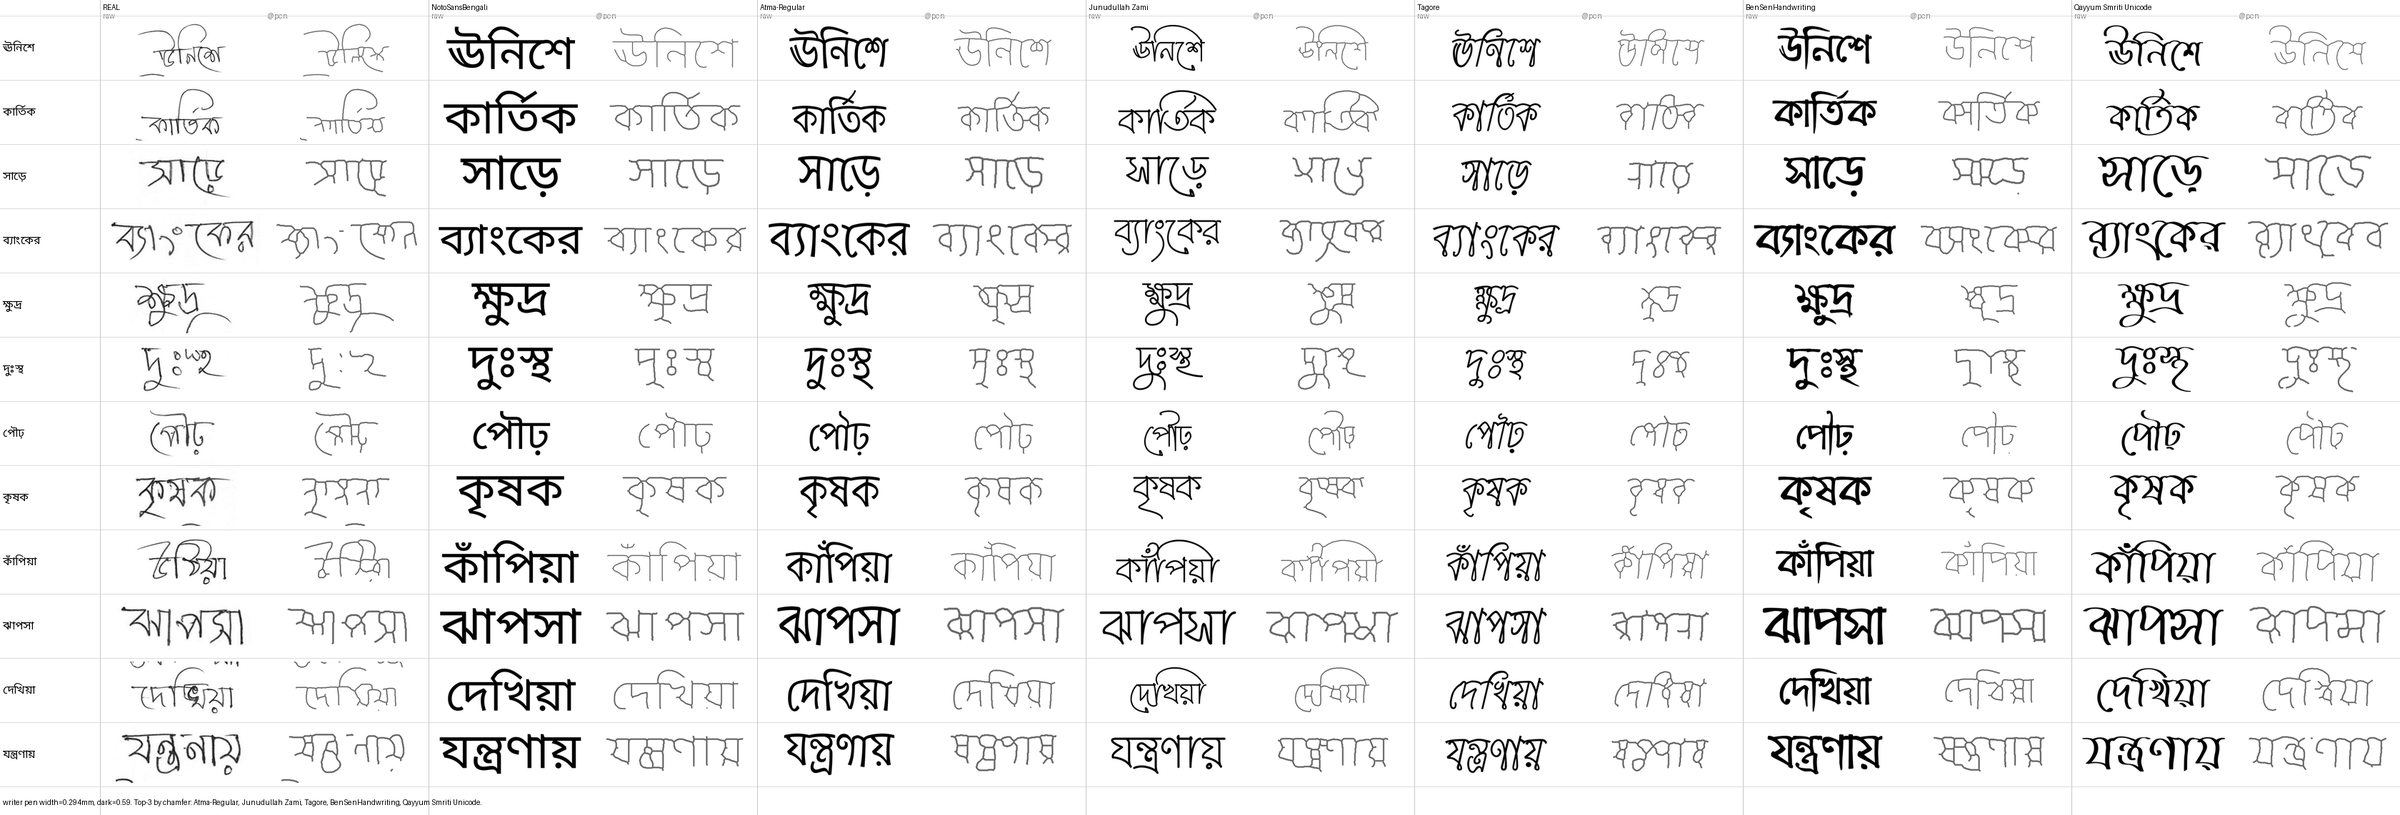
\includegraphics[width=\linewidth]{q_glyphscribe_sheet.png}
\caption{image\_2's real words (left block) against the closest fonts, each shown raw and pen-matched.}
\src{\fp{scribe_wordgen/runs/font_search/glyphscribe/sheet.png}}
\end{figure}

\subsection{R\_eval: an independent recogniser}
R\_eval answers two questions. Does pretraining on synthetic renders from the 48 fonts (37 GlyphScribe + 11 Google) help
on real handwriting? And how legible are the generator arms to a recogniser the generators never saw? The model is a
\textbf{CRNN-CTC} with 4.94\,M parameters. The input is a $64\times256$ left-aligned ink matte. A conv/ResNet stack reduces it
to $1\times64$, followed by a 2-layer BiLSTM (256 hidden) and 219 classes including blank and unk; decoding is greedy CTC
(\fp{wordgen/recog/model.py}). Synthetic words come from a 203,371-word vocabulary
(\fp{runs/R_eval/vocab_synth.tsv}). They are rendered with HarfBuzz shaping, decorative fonts are down-weighted to
0.3$\times$, and the renders are augmented for thickness, shear, rotation, baseline wave, blur, noise, paper texture and
JPEG. The real data are the 100,868 TRAIN crops. Before launch, a review fixed three blockers: wrong word pairing in
rescoring, double \texttt{crop\_ink} on cached mattes, and an augmentation roll that cut word edges. The whole chain took
1\,h\,50\,min (\fp{runs/R_eval/full_chain.log}).

\begin{table}[H]
\centering
\caption{R\_eval arms and VAL CER (codepoint, corpus; both datasets, 4,299 words; writer-bootstrap CI).}
\label{tab:reval}
\small
\begin{tabular}{@{}lllccc@{}}
\toprule
model & init & data, steps & VAL CER & BN-HTR & BW \\
\midrule
R\_font0 & -- & synthetic only, 60k & 0.4563 \ci{0.3265}{0.5338} & 0.4827 & 0.3538 \\
R\_real & -- & real TRAIN, 30k & 0.0370 \ci{0.0281}{0.0511} & 0.0308 & 0.0614 \\
\textbf{R\_font2real} & R\_font0 & real TRAIN, 30k & \textbf{0.0329} \ci{0.0245}{0.0443} & 0.0283 & 0.0507 \\
R\_mix & R\_font0 & 75\% real + 25\% synth, 30k & 0.0370 \ci{0.0267}{0.0486} & 0.0333 & 0.0514 \\
R\_real\_10 & -- & 10\% of TRAIN writers, 6k & 0.1781 \ci{0.1404}{0.2082} & 0.1731 & 0.1976 \\
R\_font2real\_10 & R\_font0 & 10\% of TRAIN writers, 6k & 0.1147 \ci{0.0797}{0.1366} & 0.1162 & 0.1090 \\
\bottomrule
\end{tabular}
\par\smallskip\footnotesize Batch 128, lr $3\times10^{-4}$, warm-up 500. R\_font2real is selected as R\_eval. For reference, the
locator's letter-unit real-crop CER is 0.056 (BN-HTR VAL) and 0.236 (BW VAL); it is not comparable.
\src{\fp{scribe_wordgen/runs/R_eval/RESULTS.md}, \fp{selection.json}, \fp{R_*/train.log}}
\end{table}

\begin{figure}[H]
\centering
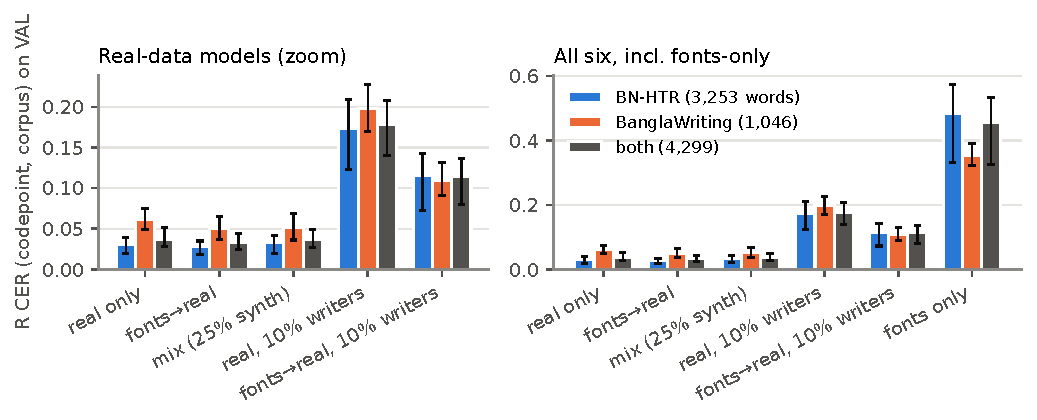
\includegraphics[width=\linewidth]{reval_models_val.pdf}
\caption{VAL CER per recogniser, by dataset (95\% writer-bootstrap CI).}
\src{\fp{runs/R_eval/RESULTS.md}}
\end{figure}

\begin{figure}[H]
\centering
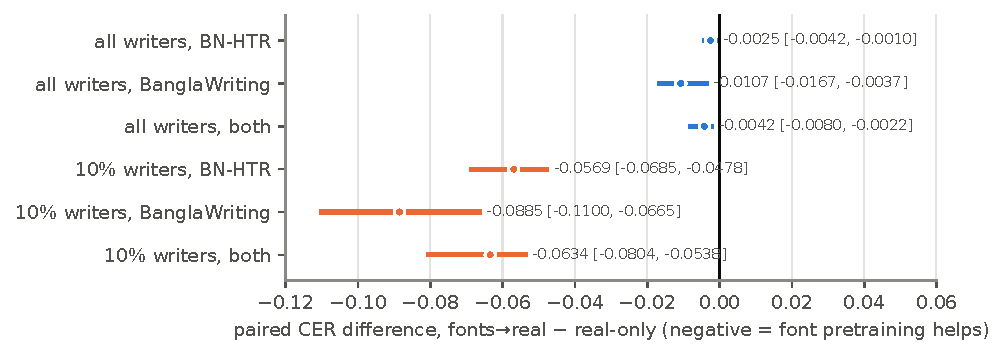
\includegraphics[width=0.85\linewidth]{reval_font_gain_forest.pdf}
\caption{Font-pretraining gain, as paired differences on the same VAL words. It is significant everywhere: small with all
writers, large with 10\% of the writers.}
\src{\fp{runs/R_eval/RESULTS.md} (paired font-pretraining gain table)}
\end{figure}

\paragraph{Findings.} Fonts alone do not transfer (0.456). As a prior they help: $-0.0042$ \ci{-0.0080}{-0.0022} overall
and $-0.0107$ \ci{-0.0167}{-0.0037} on BW with all writers. With 10\% of the writers the gain is $-0.0634$
\ci{-0.0804}{-0.0538}, from 0.178 to 0.115. Mixing synthetic data into fine-tuning (R\_mix 0.0370) does not beat plain
fine-tuning. The remaining errors are mostly lone punctuation (\bnt{,} \bnt{।} \bnt{'}) and Latin/Bengali digit confusion
(Fig.~\ref{fig:errs}).

\paragraph{OOV and TEST.} \textbf{TEST was scored once}, for R\_real and the selected model: 7,665 words.
Overall CER is 0.0429 \ci{0.0293}{0.0606} for R\_real and 0.0342 \ci{0.0228}{0.0492} for R\_font2real. On ``clean'' OOV words
(not in TRAIN and not in the synthetic vocabulary, 237 words) the two give 0.0956 and 0.0854, with overlapping CIs
(Fig.~\ref{fig:oov}). These are two separate estimates; no paired TEST difference was computed.

\begin{figure}[H]
\centering
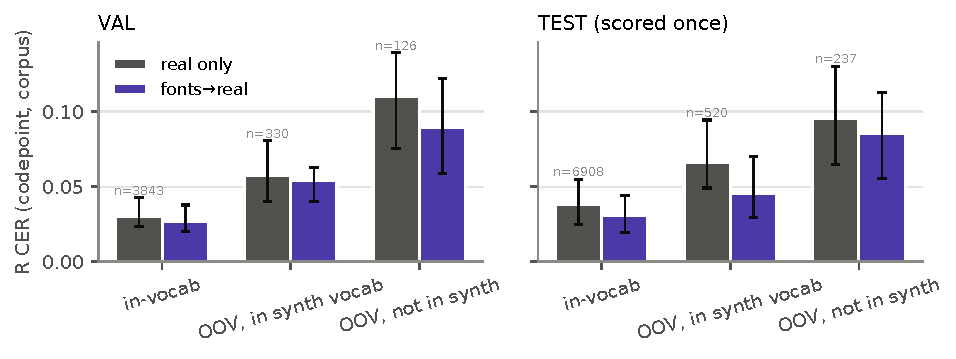
\includegraphics[width=0.9\linewidth]{reval_oov.pdf}
\caption{In-vocabulary vs OOV CER (overall). ``In synth'' means the word is in the synthetic vocabulary. TEST was scored once.}
\label{fig:oov}
\src{\fp{runs/R_eval/RESULTS.md}}
\end{figure}

\begin{figure}[H]
\centering
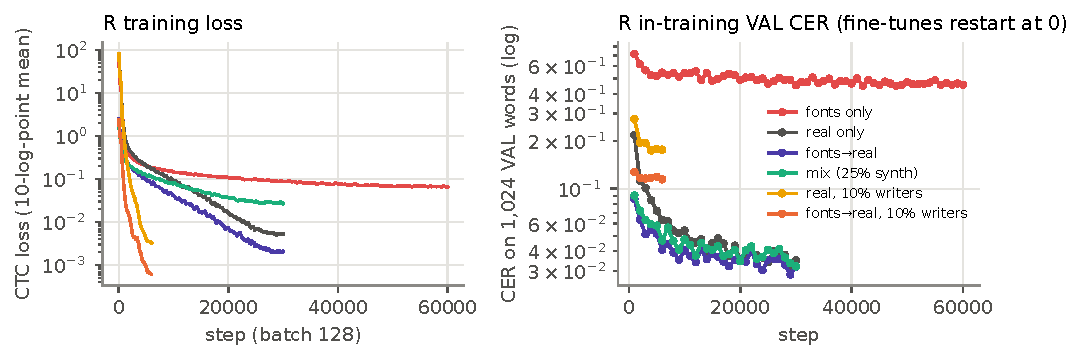
\includegraphics[width=0.95\linewidth]{curves_reval.pdf}
\caption{R learning curves. Left: CTC training loss. Right: CER on a 1,024-word VAL sample logged every 1,000 steps. This
in-training estimate is not the full-VAL number of Table~\ref{tab:reval}.}
\src{\fp{runs/R_eval/R_*/train.log}}
\end{figure}

\begin{figure}[H]
\centering
\begin{subfigure}[t]{0.50\linewidth}\centering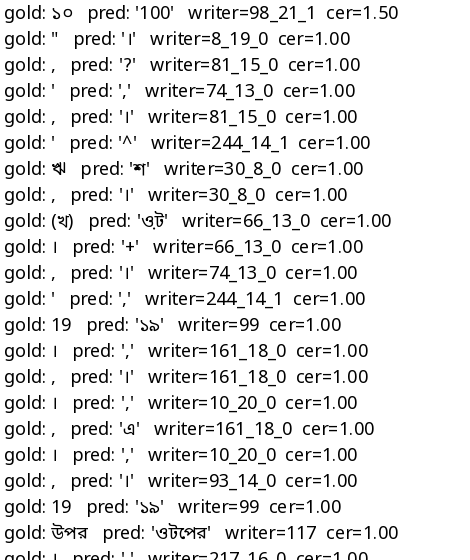
\includegraphics[width=\linewidth]{q_errors_font2real_val.png}
\caption{R\_font2real, VAL: top error rows.}\end{subfigure}\hfill
\begin{subfigure}[t]{0.40\linewidth}\centering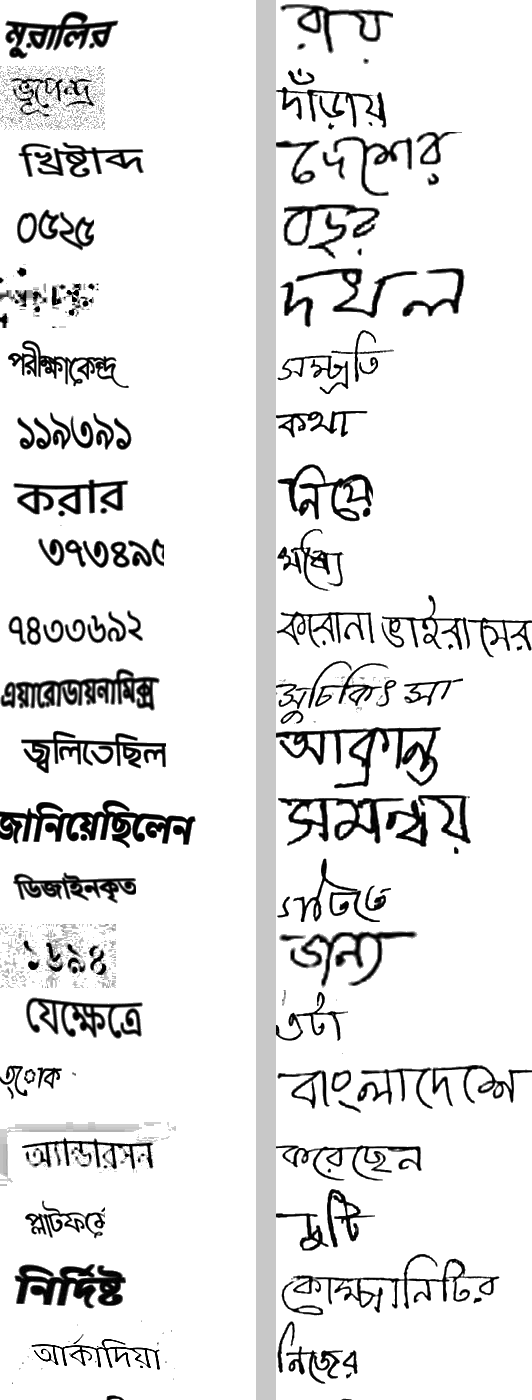
\includegraphics[width=\linewidth]{q_synth_sheet_top.png}
\caption{Synthetic training renders (top of sheet).}\end{subfigure}
\caption{R\_eval errors and synthetic data. Most residual errors are single punctuation marks and digit-script confusions
(19 read as \bnt{১৯}).}
\label{fig:errs}
\src{\fp{runs/R_eval/errors_R_font2real_val.png}, \fp{runs/R_eval/synth_sheet.png}}
\end{figure}

\subsection{Rescoring the generator arms with R\_eval}
\label{sec:rescore}
The cached eval\_v3/P1a3 renders were rescored. They are ink mattes, so they are loaded as $1-\mathrm{png}/255$ with no
re-stretch. Rows are merged on (dataset, writer, idx) against B0 and real, and on (dataset, writer, idx, seed\_k) between
diffusion arms. B0 words wider than 256\,px (about 10\%) are squashed to fit, whereas the locator truncated them.

\begin{table}[H]
\centering
\caption{Generator arms scored by R\_eval (R\_font2real), VAL, codepoint corpus CER.}
\label{tab:rescore}
\small
\begin{tabular}{@{}lcccc@{}}
\toprule
method & $n$ (all) & CER all words & $n$ ($\ge$3cp) & CER $\ge$3 codepoints \\
\midrule
real & 781 & 0.0438 \ci{0.0310}{0.0586} & 666 & 0.0424 \ci{0.0294}{0.0568} \\
B0 & 781 & 0.0302 \ci{0.0248}{0.0358} & 666 & 0.0226 \ci{0.0162}{0.0287} \\
\Bp{} t5c5 (v1 refs) & 1562 & 0.1395 \ci{0.1117}{0.1713} & 1332 & 0.1021 \ci{0.0810}{0.1264} \\
\Bp{}v2 t5c5$^{\ast}$ & 1562 & 0.1412 \ci{0.1125}{0.1749} & 1332 & 0.1024 \ci{0.0823}{0.1272} \\
P t5c5 & 1562 & 0.0905 \ci{0.0664}{0.1179} & 1332 & 0.0577 \ci{0.0402}{0.0786} \\
S t3c3 & 1562 & 0.1084 \ci{0.0804}{0.1408} & 1332 & 0.0678 \ci{0.0501}{0.0888} \\
\textbf{S t5c5} & 1562 & 0.0889 \ci{0.0652}{0.1153} & 1332 & 0.0552 \ci{0.0381}{0.0753} \\
\midrule
\multicolumn{5}{@{}l}{\emph{paired differences} (all words; $\ge$3cp)} \\
S$-$B0 & \multicolumn{2}{c}{$+0.0587$ \ci{+0.0361}{+0.0833}} & \multicolumn{2}{c}{$+0.0326$ \ci{+0.0145}{+0.0523}} \\
S$-$P & \multicolumn{2}{c}{$-0.0016$ \ci{-0.0111}{+0.0076}} & \multicolumn{2}{c}{$-0.0025$ \ci{-0.0099}{+0.0050}} \\
P$-$B0 & \multicolumn{2}{c}{$+0.0603$ \ci{+0.0375}{+0.0860}} & \multicolumn{2}{c}{$+0.0351$ \ci{+0.0174}{+0.0567}} \\
B0$-$real & \multicolumn{2}{c}{$-0.0136$ \ci{-0.0268}{-0.0021}} & \multicolumn{2}{c}{$-0.0198$ \ci{-0.0347}{-0.0067}} \\
\bottomrule
\end{tabular}
\par\smallskip\footnotesize $^{\ast}$\Bp{}v2 is not in \fp{RESULTS.md}; its row is from the full rescoring table in \fp{runs/R_eval/full_chain.log}.
\src{\fp{scribe_wordgen/runs/R_eval/RESULTS.md} (``scored with R\_eval''), \fp{runs/R_eval/rescore.csv}}
\end{table}

\begin{figure}[H]
\centering
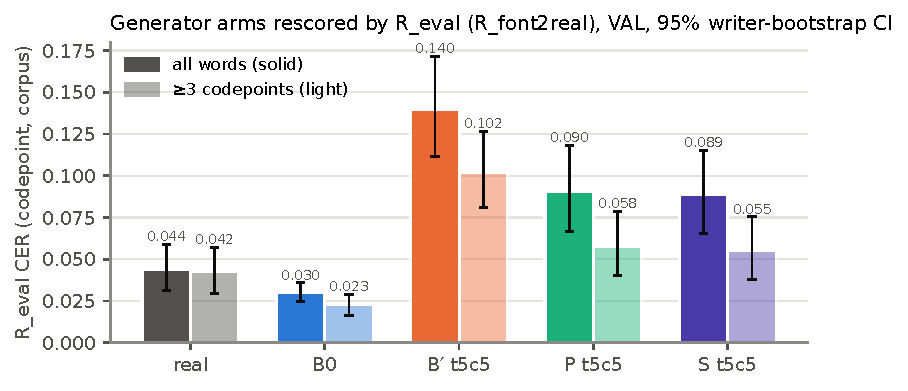
\includegraphics[width=0.88\linewidth]{reval_arms.pdf}
\caption{R\_eval CER per arm. Solid: all words. Light: words of $\ge$3 codepoints. The large drop from all words to $\ge$3cp
for P and S is partly the short-word \texttt{img\_to\_ink} artefact.}
\src{\fp{runs/R_eval/RESULTS.md}}
\end{figure}

\begin{figure}[H]
\centering
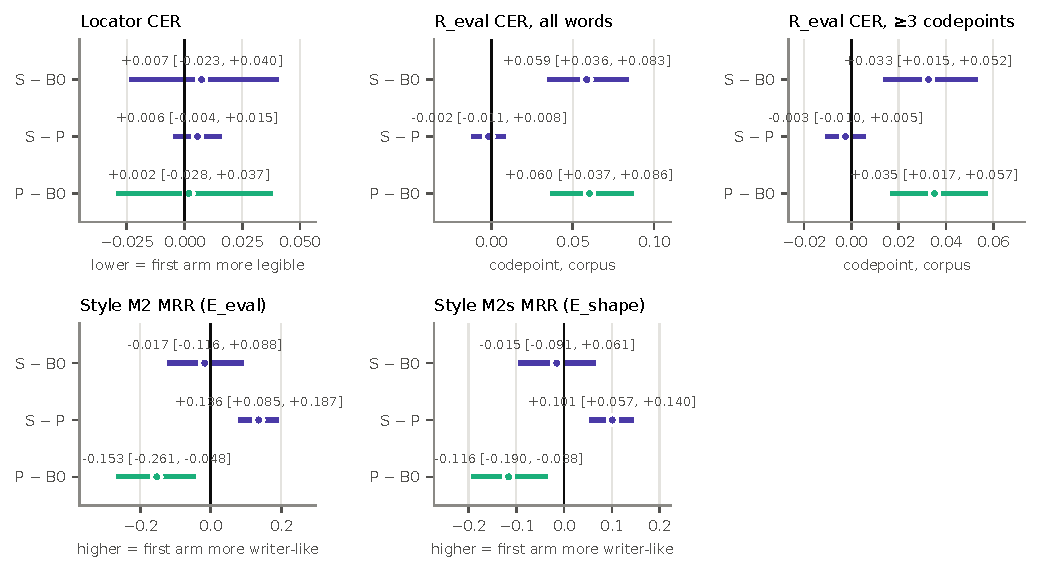
\includegraphics[width=\linewidth]{forest_paired.pdf}
\caption{Paired differences S$-$B0, S$-$P and P$-$B0, with 95\% writer-bootstrap CIs, for CER (top) and style (bottom). The
locator cannot separate the arms. R\_eval shows S and P less legible than B0 and tied with each other. Style shows S tied with
B0 and clearly better than P. \emph{The CER panels are in different units.}}
\src{\fp{runs/P1a3/eval/metrics.json}, \fp{runs/R_eval/RESULTS.md}}
\end{figure}

\paragraph{How to read the legibility gap.}
\begin{itemize}
\item \textbf{The short-word artefact explains only part of it.} S's CER is 0.089 on all words and 0.055 on $\ge$3cp
  words. The all-word gap to B0 ($+0.059$) is inflated by the legacy \texttt{img\_to\_ink} smudge on lone glyphs. The
  $\ge$3cp gap, $+0.033$ \ci{+0.015}{+0.052}, \textbf{remains significant}. S really is less legible than B0, by about
  1.3$\times$ real's CER on $\ge$3cp words. (One of the gathered notes called the gap ``an artefact of short-word ink
  normalisation''; that overstates it.)
\item \textbf{Left-alignment caveat.} A later CPU check (Opus review, \fp{runs/S_ocrloss/REVIEW.md}, \S A) found a framing
  mismatch. R\_eval was trained on left-aligned crops, but S/P renders are centred by \texttt{fit\_canvas}. On 400 cached PNGs
  per arm, the median left margin is 54\,px for S, 6\,px for real and 0\,px for B0. Centring real crops raises R\_font2real
  micro-CER from 0.047 to 0.096. Left-shifting S renders moves S only from 0.099 to 0.092 ($n=800$). So layout explains only
  about 0.007 of S's $\approx$0.06 gap to B0; most of the gap is real legibility. These are that review's subsample numbers,
  not the RESULTS.md protocol.
\item \textbf{CER is legibility, not fidelity.} B0 is read \emph{more} easily than the writers' own crops ($-0.0136$
  \ci{-0.0268}{-0.0021}). A clean, font-like render beats real handwriting under any recogniser. CER can therefore only say
  that an arm is legible enough. Arms are ranked on CER together with style and pen.
\end{itemize}

%=============================================================================
\section{Bugs found and lessons}
\label{sec:bugs}

Most of the project's large swings in conclusions came from measurement, not from models. Table~\ref{tab:pitfalls} collects
every pitfall that changed a number or a decision.

\begin{longtable}{@{}p{3.5cm}p{6.6cm}p{5.4cm}@{}}
\caption{Measurement pitfalls and bugs, with their effect and fix.}\label{tab:pitfalls}\\
\toprule
pitfall & what happened & effect / fix \\
\midrule
\endfirsthead
\toprule
pitfall & what happened & effect / fix \\
\midrule
\endhead
\bottomrule
\endfoot
Uncapped CER (P1a) & 1-character punctuation targets read as 23--29 characters; 15\% of words had CER $>1$ & CER $>1$ was an artefact; cap at 1 and exclude punctuation \\
Grey-box failures (P1a) & writer 117's grey refs led to grey rectangles; \texttt{img\_to\_ink} turned them into ``ink'', so w/core $\approx$100 & mean w/core $\approx$4 was one writer; whiten refs, then bgnorm2 \\
Eval asymmetry (P1a) & real/B0 tight and left-aligned, generated centred on a 256 canvas; B0 $>$256\,px truncated & 0.04--0.05 CER bias; left-align, report it \\
Same noise for every word (P1a) & all words sampled from seed 0 & correlated outputs; per-word seeds \\
\textbf{CFG-null bug} (P1a$'$) & content map and tokens in both CFG branches, so content was never guided & ``\Bp{} NO-GO, 0.550'' inverted to ``best arm, 0.188''; joint null \\
Integer EDT pen (eval\_v2) & $2\,\mathrm{EDT}-1$ takes values $\{1,1.83,3,\dots\}$ on 64\,px & 1.8--2.2$\times$ reported vs 1.13--1.36$\times$ true; sub-px/core metric \\
Underpowered OOV gate (P1a$'$) & 15 OOV words, one word carried the effect; sign-inverted gate code & replaced by OOV on all 20 writers, $\ge$2 seeds \\
Off-by-one vocab size (eval\_v2) & \texttt{vocab\_size=len(vocab)} where training used $+1$ for pad/OOV & fixed at both call sites \\
bg-fail misses faint blotches & writer 117 blotches are faint (ink 0.18--0.5) & faint-blotch score added \\
\textbf{\texttt{img\_to\_ink} short-word smudge} & 5th-percentile floor stretches paper texture to black on lone glyphs (2--3\% ink) & short-word CER/blotch for P/\Bp/S inflated; \texttt{min\_span=100} (opt-in), caches not yet rescored \\
\textbf{Gradient checkpoint bug} (S) & side-channel attributes reset before the checkpoint recompute & S diverged twice; fixed and tested \\
Cached PNGs are mattes & saved as $255(1-\text{ink})$; re-running \texttt{crop\_ink} re-stretches ink & read with $1-\mathrm{png}/255$ (blocker fixed before R\_eval) \\
Wrong word pairing (R\_eval) & seeds differ across arms (B0/real 1, diffusion 2) & merge on (dataset, writer, idx, seed\_k), never zip \\
Augmentation cut words (R\_eval) & symmetric $\pm$12\% roll deleted word edges & roll only into empty columns \\
B0 wider than 256\,px & $\approx$10\% of B0 words, up to 628\,px & locator truncates, R\_eval squashes: B0 rows differ between the two \\
\textbf{Locator vs R\_eval units} & letter-unit capped per-word mean vs codepoint corpus ratio & never compare across the two \\
\textbf{Recogniser CER $\neq$ fidelity} & B0 beats real crops under R\_eval & rank arms with style and pen too \\
R\_eval framing & R trained left-aligned, S/P centred & $\approx$0.007 of S's gap; left-shift in future evals \\
\midrule
\textbf{Biased e2e C2ST} (layout) & pooled OOF AUC with one label per group; floor 0.34 / 0.115 & e2e\_unfit, e2e\_unfit\_ink C2ST not comparable; balanced folds \\
Shuffled real as ``floor'' & breaks gap--width relation & real null is within-page split, 0.496 \\
Per-word wobble overshoot & line-scale inflation applied to every word & up to 2$\times$ wobble; leverage correction \\
Selection on TEST (layout) & every choice compared on TEST & optimistic by $\sim$1 sd; VAL check added \\
Planner history across pages & history 56--72 lines vs $\le$16 in training; slope random walk & per-page reset \\
Survivor bias in e2e & detector splits steep/bowed lines; metrics see survivors & slope/drift W1 not comparable across runs \\
Ink-extent threshold & \texttt{INK\_LEVEL} 0.35 vs page Otsu $\approx$0.39 & $+0.067$\U{} gap bias \\
Uncontrolled 2-D FFT & block height alone separates real from generated (AUC 0.985) & only the controlled test is valid \\
Fourier ``17$\times$'' & compared an unrealisable continuous trace with a floor artefact & fair: Fourier 0.668 vs v1 0.702 \\
Vacuous tests (layout) & noise-floor tolerance $|$AUC$-0.5|<0.4$; tests on fake models & tightened to 0.15; 70 tests \\
\end{longtable}
\src{\fp{runs/P1a/REVIEW.md}, \fp{runs/P1a2/REVIEW.md}, \fp{EXPERIMENTS.md} (Known pitfalls), \fp{runs/S_ocrloss/REVIEW.md} \S A
(framing only), \fp{scribe_layout_v2/report/FACTS.md}, \fp{scribe_layout_v2/runs/review_opus.md}}

\paragraph{Lessons.}
\begin{enumerate}
\item \textbf{Review the sampler and the metric before the model.} Two verdicts (P1a$'$ \Bp, the pen ratio) flipped because of
  the evaluation code, not the model.
\item \textbf{Every metric needs a null and a ceiling measured in the same pipeline}: real-vs-real C2ST, real-crop CER, real
  MRR, fonts as the style null. A null of 0.34 instead of 0.5 is a protocol failure, not a result.
\item \textbf{Measure like with like.} Sub-pixel width relative to letter size, the same canvas convention, the same framing
  as the recogniser's training data.
\item \textbf{Keep a selection-free split.} TEST-selected layout gains shrank or vanished on VAL.
\item \textbf{Legibility is necessary but not sufficient.} A recogniser rewards font-like renders, so it cannot rank
  fidelity.
\end{enumerate}

\subsection{Contradictions between sources}
\label{sec:contradictions}
\begin{itemize}
\item \textbf{Fourier ``17$\times$''.} \fp{scribe_layout_fourier/runs/results.md} still states it. \fp{FACTS.md} corrects it
  with the fair comparison (0.668 vs 0.702). This report follows FACTS.
\item \textbf{fft2d uncontrolled section.} The results file reports high AUCs that are confounded; only its controlled section
  is used here.
\item \textbf{R\_eval row label (resolved).} \fp{runs/R_eval/RESULTS.md} lists \texttt{Bp\_t5c5} (0.1395 / 0.1021) but not
  \Bp{}v2; the full table in \fp{runs/R_eval/full_chain.log} scores both, and \texttt{Bv2\_t5c5} is 0.1412 / 0.1024, as in
  \fp{EXPERIMENTS.md}.
\item \textbf{The 41 BW words missing from the R\_eval cache (resolved).} An early attribution to a Unicode nukta
  mismatch was wrong: they are the 41 \texttt{measure\_rows} failures of the T0 index (\fp{runs/T0/REPORT.md} \S4.2).
\item \textbf{Writer disjointness in hcr/996.} The v1 layout report says TEST lines are by unseen writers. \fp{FACTS.md} says
  writers likely repeat across texts and that this cannot be verified (no writer IDs).
\item \textbf{The gathered notes} contain errors that this report does not repeat. Note 04 calls S's R\_eval gap an artefact
  (only part of it is). It says the second diverged S run was stable (its rolling loss rose to 0.108 by step 1,050).
  It says ``CER capped'' for R\_eval (the corpus CER is not capped). Note 05 gives a TEST paired diff that is not in any source
  (dropped). Note 03 mislabels P1a\_B as \Ap. Note 06 has invented column lists.
\end{itemize}

%=============================================================================
\section{Discussion}
\label{sec:discussion}

\paragraph{What works.}
\begin{itemize}
\item \textbf{Learned layout.} The planner is small (seven 1-D MDNs) and trains in seconds. It reproduces real spacing
  dependence (gap lag-1, gap--width, slope persistence) and brings line C2ST from 0.98 to about 0.53 at plan level. It is
  integrated in BS with clearance, margins and per-page resets.
\item \textbf{Content through tokens.} Grapheme tokens in cross-attention carry word identity (content-only CER 0.199); a
  painted map does not.
\item \textbf{Reference tokens for style.} S closes the style gap to B0 ($-0.017$, n.s.) and beats every other diffusion arm
  by about 0.14 MRR.
\item \textbf{Pen.} Rebalancing plus a pen input brings the raw ratio from 1.29--1.30 (\Bp) to 1.13--1.15. Post-hoc
  calibration reaches 1.06.
\item \textbf{Fonts as a recogniser prior}, especially with little real data (0.178$\to$0.115 with 10\% of writers).
\end{itemize}

\paragraph{What does not (yet).}
\begin{itemize}
\item \textbf{Legibility of the diffusion arms.} On words of $\ge$3 codepoints S and P are about 1.3$\times$ real's R\_eval
  CER and 2.4$\times$ B0's. This is now the main gap.
\item \textbf{S does not beat B0 on style.} It ties. On BN-HTR, B0 is close to real (0.883 vs 0.916); on BW all arms are
  far from real (S 0.523, B0 0.500, real 0.789).
\item \textbf{The pen knob in S is inert} (slope 0.03), so pen control must come from calibration.
\item \textbf{Page-level integration.} Text renders small on BW pages; P draws dashes as bars; short words carried the smudge
  artefact.
\item \textbf{Layout gaps.} $x_\mathrm{start}$ is the weakest learned quantity. End-to-end C2ST (0.72 / 0.62 with context)
  is far from the 0.53 floor, partly because of extraction survivor effects.
\end{itemize}

\paragraph{Open problems.} (1)~Legibility without losing style. A recogniser-guided objective is the obvious lever, but it
must not reuse R\_eval, which would make the evaluation circular. (2)~Thin pens like image\_2 (1.6\,px at 64\,px) need a
larger canvas; the review recommended $128\times512$ \texttt{fit\_canvas}. (3)~The latent writer-style layout model's context
mismatch. (4)~A correlated-wobble calibration for the per-word unfit correction. (5)~The hcr writer-identity question, which
limits both layout splits and any hcr content-matched style metric.

%=============================================================================
\section{Next steps}
\label{sec:next}
\begin{enumerate}
\item \textbf{Running now (no results cited here):}
  \begin{itemize}
  \item \emph{smudge-fix rescore}: rescore all arms together with \texttt{min\_span} and re-extracted inks, removing the
    short-word artefact from the S/P vs B0 gap;
  \item \emph{best-of-N recogniser selection}: sample several candidates per word and keep the most legible;
  \item \emph{recogniser-loss fine-tuning}: fine-tune S with an auxiliary CTC loss. Its review asks that it be scored both
    as-is and left-aligned, with a left-margin diagnostic, so that a ``move ink left'' shortcut is not mistaken for legibility.
  \end{itemize}
\item Add left-aligned R\_eval scoring as a standard column for every generator arm.
\item Fix BW page scale and dash words at integration; re-render the page sheets.
\item Revive pen control in S (knob dropout or a stronger embedding), or adopt calibration as the official pen path.
\item P1b at $128\times512$ \texttt{fit\_canvas}, warm-started from S, for thin-pen writers.
\item Per-writer test-time adaptation (LoRA) with leave-crop-out stopping and the M6 copy check.
\item \textbf{Checkpoint C}: one TEST evaluation of the final configuration against B0 and the baselines, with all metrics.
\end{enumerate}

\appendix
%=============================================================================
\section{Reproduction}
\label{app:repro}
Python is \fp{/home/hpc4090/shyan/ocr/venv/bin/python}. Run one GPU job at a time under the shared lock
\fp{runs/.gpu.lock}. Working directory: \fp{scribe_wordgen/} unless noted.

\begin{table}[H]
\centering
\small
\begin{tabular}{@{}p{3.4cm}p{12.2cm}@{}}
\toprule
step & command / path \\
\midrule
this report & \texttt{cd reports/final \&\& python make\_figs.py \&\& latexmk -xelatex report.tex} \\
data index, splits & \fp{wordgen/data/index.py} $\to$ \fp{data_cache/index_{bnhtr,bw}.csv}, \fp{data_cache/splits.json} \\
BW crops (missing on disk) & \fp{wordgen/recog/bw_regen.py} (in memory, from \fp{banglawriting/converted/}) \\
eval\_v3 & \texttt{python -m wordgen.eval.eval\_v3 --stage gen|import|score|validate|report|sheets} $\to$ \fp{runs/eval_v3/} \\
style metric & \texttt{python -m wordgen.eval.style\_metric --stage all} $\to$ \fp{runs/style_eval/} \\
P/S training & \fp{wordgen/train/train_diffusion3.py}; checkpoints \fp{runs/P1a3/{P,S}/unet3_final.pt} \\
P/S evaluation & \fp{wordgen/eval/eval_p1a3.py} $\to$ \fp{runs/P1a3/eval/report_tables.txt} \\
pen calibration & \fp{wordgen/pen/calibrate.py} $\to$ \fp{runs/pen_calib/} \\
R\_eval chain & \fp{runs/R_eval/full_chain.sh} (train, select, TEST once, rescore) $\to$ \fp{runs/R_eval/RESULTS.md} \\
page sheets & \fp{wordgen/integrate/page_sheets.py} $\to$ \fp{runs/page_sheets/sheets/} \\
layout model & \texttt{cd scribe\_layout\_v2}; train with \fp{configs/default_unfitw_dc.yaml}; default \fp{runs/default_unfitw_dc/model.pt} \\
layout 5-seed compare & \fp{scribe_layout_v2/runs/compare_unfitw/compare_5seed*.py} \\
layout end to end & \fp{scribe_layout_v2/runs/e2e_final/} (results.md, results.json) \\
\bottomrule
\end{tabular}
\end{table}

\section{Glossary}
\begin{description}[style=nextline,leftmargin=2.8cm,labelwidth=2.6cm]
\item[B0] BengaliScribe's shipped font-prior GAN word generator.
\item[B3] DiffusionPen fine-tuned on all BW writers (\texttt{dp\_words\_b64}); a probe/baseline only.
\item[\Ap, \Bp] P1a$'$ diffusion arms: text only, and text + grapheme tokens.
\item[P, S] P1a3 arms: \Bp{} + pen knob + null style (P); + reference tokens in decoupled cross-attention (S).
\item[t$X$c$Y$] text guidance $X$, content guidance $Y$ in classifier-free guidance.
\item[CFG null] the unconditional branch; must drop text, map and tokens jointly.
\item[core, U] body height under the matra; U = a page's median word core height (layout unit, $\approx$3.5\,mm).
\item[matra] the Bengali headline stroke.
\item[locator CER] CER from BS's \texttt{attn\_locator}; letter units, capped per-word mean.
\item[R\_eval] the independent CRNN-CTC recogniser (R\_font2real); codepoint corpus CER.
\item[cp] codepoint.
\item[M2 / M2s] writer-ID MRR with E\_eval (shape + pen) / E\_shape (skeleton only).
\item[MRR] mean reciprocal rank of the true writer among candidates.
\item[pen ratio] median over writers of (generated / own real) sub-pixel width per core.
\item[bg-fail, blotch] background-failure and faint-blotch rates.
\item[OOV] target word not in the training texts (for R\_eval: also split by the synthetic vocabulary).
\item[C2ST] classifier two-sample test; AUC 0.5 = indistinguishable.
\item[W1, KS] Wasserstein-1 distance and Kolmogorov--Smirnov statistic between marginals.
\item[MDN] mixture-density network head.
\item[unfit / unfitw / dc] layout targets inflated for fit shrinkage (line table / per-word leverage) / curvature deconvolution.
\item[e2e] end to end: BS render $\to$ real detector $\to$ same extraction.
\item[VAL / TEST] writer-disjoint (words) or text-disjoint (layout) evaluation splits.
\end{description}

\end{document}
